\documentclass[oneside,a4paper,11pt]{book}
\usepackage[utf8]{inputenc}
\usepackage{svg}
\usepackage[italian]{babel}
\usepackage{float}
\usepackage{fancyvrb}
\usepackage{titling}
\usepackage[margin=1in,footskip=0.25in]{geometry}
\usepackage{listings}
\usepackage[DIV=12,BCOR=2mm,headinclude=true,footinclude=false]{typearea}
\usepackage{color, colortbl,xcolor}
\usepackage[hidelinks]{hyperref}
\usepackage{tcolorbox}
\usepackage{chngcntr}
\usepackage{calc}
\usepackage{amssymb}
\usepackage{subcaption}
\usepackage{amsthm}
\usepackage{ulem}
\usepackage{proof}
\usepackage{amsfonts}
\usepackage{mathtools}
\usepackage{stmaryrd}
\usepackage{parskip}
\usepackage{cancel}
\usepackage{forest}
\usepackage{listings}
\usepackage{mathrsfs}
\usepackage{enumitem}
\usepackage{makecell}
%TIKZ environment
\usepackage{tikz}
\usepackage{pgfplots}
\pgfplotsset{compat=1.18}
\usepackage{fancyhdr}
\fancypagestyle{plain}{\fancyhf{}\renewcommand{\headrulewidth}{0pt}} % To clear page numbers from footer, and header line at the start of every chapter

\usepackage{color}
\usepackage{listings}
\usepackage{caption}

\newcounter{nalg}[chapter] % defines algorithm counter for chapter-level
\renewcommand{\thenalg}{\thechapter .\arabic{nalg}} %defines appearance of the algorithm counter
\DeclareCaptionLabelFormat{algocaption}{Algorithm \thenalg} % defines a new caption label as Algorithm x.y

\lstnewenvironment{algorithm}[1][] %defines the algorithm listing environment
{   
    \refstepcounter{nalg} %increments algorithm number
    \captionsetup{labelformat=algocaption,labelsep=colon} %defines the caption setup for: it ises label format as the declared caption label above and makes label and caption text to be separated by a ':'
    \lstset{ %this is the stype
        mathescape=true,
        frame=tB,
        numbers=left, 
        numberstyle=\tiny,
        basicstyle=\scriptsize, 
        keywordstyle=\color{black}\bfseries\em,
        keywords={,input, output, return, datatype, function, in, if, else, foreach, while, begin, end, 
                    const, int, void,} %add the keywords you want, or load a language as Rubens explains in his comment above.
        numbers=left,
        xleftmargin=.04\textwidth,
        #1 % this is to add specific settings to an usage of this environment (for instnce, the caption and referable label)
    }
}
{}

\usepackage{bussproofs}


\pagestyle{fancy}
\fancyhf{}% Clear header/footer
\fancyhead[L]{\nouppercase\leftmark}
\fancyhead[R]{\thepage}

\usetikzlibrary{positioning,shapes.geometric,arrows.meta,matrix,automata,decorations.pathmorphing,patterns,decorations.pathreplacing}
\tcbuselibrary{skins}
\counterwithin{figure}{section}
%Nuovi comandi
\newcommand\myeq{\stackrel{\mathclap{\normalfont\mbox{def}}}{=}}
\newcommand\prodG{\stackrel{\mathclap{\normalfont\mbox{\tiny{G}}}}{\Longrightarrow}}
%asmthm
\newlength{\marginlabelsep}\setlength{\marginlabelsep}{0.5em}
\newtheoremstyle{italicstyle} %% Name
  {} %% <- Space above (empty = default = \topsep = 8.0pt plus 2.0pt minus 4.0pt)
  {} %% <- Space below (empty = default = \topsep = 8.0pt plus 2.0pt minus 4.0pt)
  {\itshape} %% <- Body font
  {} %% <- Indent amount (empty = no indent, \parindent = just that)
  {\bfseries} %% <- Thm head font
  {} %% <- Punctuation after thm head
  {1pt} %% <- Space after thm head (or " " or \newline) (default: 5pt plus 1pt minus 1pt)
  {\vtop to 0pt{\llap{\thmname{#1}\hskip\marginlabelsep}
                \llap{\thmnumber{#2}\hskip\marginlabelsep}}\thmnote{#3\\}%
  }
\newtheoremstyle{normStyle} %% Name
  {} %% <- Space above (empty = default = \topsep = 8.0pt plus 2.0pt minus 4.0pt)
  {} %% <- Space below (empty = default = \topsep = 8.0pt plus 2.0pt minus 4.0pt)
  {\normalfont} %% <- Body font
  {} %% <- Indent amount (empty = no indent, \parindent = just that)
  {\bfseries} %% <- Thm head font
  {} %% <- Punctuation after thm head
  {1pt} %% <- Space after thm head (or " " or \newline) (default: 5pt plus 1pt minus 1pt)
  {\vtop to 0pt{\llap{\thmname{#1}\hskip\marginlabelsep}
                \llap{\thmnumber{#2}\hskip\marginlabelsep}}\thmnote{#3\\}%
  }
\theoremstyle{italicstyle}
\newtheorem{corollary}{Corollario}[section]
\newtheorem{notazione}{Notazione}[section]
\newtheorem{lemma}{Lemma}[section]
\newtheorem{definizione}{Definizione}[section]
\newtheorem{nota}{Nota}[section]
\newtheorem{exercise}{Esercizio}[section]



\theoremstyle{normStyle}
\newtheorem{exmp}{Esempio}[section]
\newtheorem{theorem}{Teorema}[section]
\newtheorem{proposizione}{Proposizione}[section]
\tcbuselibrary{listings,skins}
\newtcblisting{mylisting}[2][]{
        arc=0pt, outer arc=0pt,
    listing only, 
    title=#2,
    #1,
    listing options= {escapechar=|}
}

\newcommand{\myboxedtext}[2][rectangle,draw]{%
        \tikz[baseline=-0.6ex] \node [#1]{#2};}%
\title{Linguaggi}
\author{Alessio Gjergji}
\date{Anno accademico 2022 - 2023}

\begin{document}
\hypersetup{ %set true if you want colored links
    linktoc=all,     %set to all if you want both sections and subsections linked
    linkcolor=black,  %choose some color if you want links to stand out
}
\maketitle
\tableofcontents
\chapter{Introduzione al corso}
\section{Come nascono i linguaggi}
Per arrivare a comprendere l'importanza dello studio dei linguaggi 
di programmazione da un punto di vista generale, è importante 
capire quali necessità hanno portato alla nascita e all'evoluzione 
dei linguaggi di programmazione.

Il principale problema dell'informatica consiste nel voler far eseguire 
ad una macchina \textbf{algoritmi} che manipolano \textbf{dati}:

Ma cosa è una macchina su cui possiamo eseguire programmi che 
manipolano dati? In generale è una macchina \textbf{programmabile}, 
ovvero un calcolatore che può eseguire insiemi di istruzioni (\textit{passi 
di calcolo dell'algoritmo}) che chiamiamo programmi, ricevuti come input (\textbf{macchine 
universali}.)

In particolare i computer moderni hanno un'architettura che nasce 
dall'architettura di Von Neumann. Questa è una tipologia di architettura 
hardware per macchine programmabili, con programma memorizzato, dove 
i dati ed istruzioni condividono la stessa area di memoria. 

Quindi per operare su questa architettura di che linguaggi abbiamo 
bisogno? Essenzialmente dobbiamo istruire la CPU (\textit{eseguire algoritmi}) 
per operare sui dati in memoria. È proprio la struttura essenziale di 
questa architettura che ha messo al centro il concetto di linguaggio 
di programmazione la cella di memoria. Comunemente ad esempio, anche 
a livello formale, lo stato di esecuzione di una macchina è descritto attraverso 
i valori contenuti nelle sue celle di memoria.

Il primo linguaggio che permette di programmare tale architettura è 
quello che si basa sull'implementazione stessa dell'architettura, ovvero solo 
sulla base del funzionamento degli elementi hardware che la costituiscono e che, comportandosi
come interruttori possono trovarsi solo in due stati: acceso e spento. La programmazione 
con schede perforare si basa esattamente su questo linguaggio a due valori, ovvero il 
linguaggio binario.

Di fatto la macchina hardware è in grado di interpretare solo il 
linguaggio \textbf{binario}, ovvero un linguaggio costituito esclusivamente 
da stringhe di bit.
\subsection{Dal linguaggio binario ai linguaggio ad alto livello}
Abbiamo osservato che nell'architettura hardware dari e programmi 
condividono la stessa area di memoria, questo significa anche che a basso 
livello sono rappresentati nello stesso modo, con lo stesso linguaggio 
binario. In altre parole \textbf{dati e istruzioni hanno lo stesso formato}: 
una stringa di bit può essere sia un dato che una o più istruzioni.

Quindi il linguaggio binario è un linguaggio di programmazione perché 
permette di programmare una macchina, ma chi lo implementa deve essere 
in grado di distinguere stringhe che rappresentano dati da stringhe 
che rappresentano istruzioni che manipolano dati.

La possibilità di vedere i programmi come dati passati in input ad 
una macchina (\textit{universale}) è stato un passaggio fondamentale 
nella storia dell'informatica per avviare al concetto di macchina 
programmabile, ma allo stesso tempo ha comportato la difficoltà intrinseca 
di riuscire a distinguere dati e istruzioni, in un linguaggio fatto di soli 
due simboli. Difficoltà che ad esempio rende molto difficile il processo 
di \textit{disassembly} e di \textit{decompilazione}. Infatti, dati 
e istruzioni, pur avendo la stessa rappresentazione a livello macchina, 
vanno trattati in modo sostanzialmente diverso: il dato viene manipolato, 
l'istruzione viene interpretata.

Per queste ragioni abbiamo bisogno di linguaggi diversi da quello binario, 
linguaggi che un essere umano possa capire e manipolare, ma allo stesso 
tempo che siano interpretabili dalla macchina. Questi saranno i 
linguaggi ad alto livello che in modo poi automatico, mediante compilazione 
o interpretazione vengono eseguiti a livello macchina.
\subsection{Cosa significa programmare}
Per quanto detto, un linguaggio di programmazione deve permettermi 
di \textbf{agire} sulla macchina per manipolare \textbf{dati}, quindi un linguaggio
di programmazione deve essere uno \textbf{strumento che permette di 
descrivere algoritmi e rappresentare dati}.

Un linguaggio di programmazione deve per prima cosa permettere di superare 
la difficoltà di distinguere dati da istruzioni, fornendo una chiara 
distinzione tra dato e istruzione.

\subsubsection{Algoritmi}
Un algoritmo è una sequenza di passi elementari il cui significato 
è il calcolo di una funzione. In altre parole, un algoritmo scompone 
un calcolo complesso in passi elementari di computazione. Un algoritmo 
è quindi un concetto astratto, e la sua forma concreta è la definizione 
di un programma, ovvero una sequenza finita di istruzioni.

Ci servono quindi strumenti per scrivere precisamente programmi che 
descrivono/implementano algoritmi. I \textbf{linguaggi di programmazione} 
nascono quindi proprio per questo: sono \textbf{linguaggi formali le cui 
frasi sono programmi, ovvero forme concrete di algoritmi eseguibili/interpretabili 
da una macchina}.

\begin{tcolorbox}[title={Algoritmo}]
Un algoritmo è quindi una sequenza finita di passi primitivi di calcolo 
descritti mediante una frase ben formata (\textit{programma}) in un linguaggio 
di programmazione. 
\end{tcolorbox}
Quindi per specificare ed eseguire un algoritmo abbiamo bisogno 
di scrivere programmi e per scrivere programmi abbiamo bisogno di strumenti che 
di permettono di farlo, ovvero di linguaggi di programmazione.

Va osservato che non esiste una corrispondenza precisa tra programmi 
e algoritmi:
\begin{itemize}
  \item Un programma non è necessariamente un algoritmo, in quanto 
  una frase grammaticalmente corretta può non avere significato.
  \item Lo stesso algoritmo può avere concretizzazioni diverse, ovvero lo stesso 
  algoritmo può essere implementato da infiniti programmi.
\end{itemize}
A questo punto si aprono diverse questioni che verranno viste in seguito:
\begin{itemize}
  \item Dobbiamo stabilire le regole che permettono di costruire 
  frasi grammaticalmente corrette in un linguaggio: \textbf{Grammatiche 
  Context-free}.
  \item Dobbiamo stabilire gli elementi base (\textit{terminali della grammatica})
  di cui abbiamo bisogno per definire i programmi in un linguaggio di programmazione: 
  \textbf{Categorie sintattiche}.
  \item Il significato di quale categoria sintattica descrive l'insieme dei 
  passi elementari di computazione \textbf{Comandi}.
\end{itemize}
\subsubsection{Dati}
I dati sono informazioni memorizzate concretamente in celle di memoria 
e astratte in elementi che il linguaggio di programmazione può manipolare:
le \textbf{variabili}.
\subsection{Cosa sono i linguaggi di programmazione}
Il programma è la concretizzazione di un algoritmo che manipola 
dati, manca però un altro ingrediente, ovvero la \textbf{trasformazione} di dati 
che l'algoritmo vuole eseguire, questa trasformazione è il significato dell'algoritmo, 
la semantica del programma. Quindi, dare semantica ad un programma significa 
descrivere matematicamente l'effetto dell'esecuzione del programma sui dati.

Il programma costituisce ciò che chiameremo \textbf{sintassi}, mentre l'effetto 
dell'esecuzione del programma, la trasformazione dei dati eseguita, 
costituisce ciò che chiameremo \textbf{semantica}.

Le trasformazioni di dati sono funzioni sui dati e, in quanto tali,
sono notoriamente descrivibili mediante linguaggio matematico, il quale 
è sicuramente rigoroso e formale. Questo significa che il linguaggio 
della matematica può essere considerato linguaggio di programmazione (\textit{di 
fatto esiste un paradigma detto funzionale che una le funzioni come strumento di 
computazione}), ma ha tre importanti mancanze collegate tra loro:
\begin{enumerate}
  \item non sempre permette rappresentazioni finite di oggetti infiniti;
  \item non sempre fornisce direttamente un metodo di calcolo di ciò che si vuole 
  rappresentare;
  \item non permette di rappresentare titti i problemi calcolabili.
\end{enumerate}
Consideriamo il punto $(1)$, questo è importante perché il programma 
è necessariamente un oggetto finito, mentre il calcolo di funzione richiede 
l'esecuzione di un insieme di passi primitivi, che però possono essere 
infiniti. Alla base della teoria della calcolabilità troviamo proprio 
la necessità di ammettere computazioni divergenti per poter catturare 
tutto ciò che effettivamente può calcolare.

Questo significa che dobbiamo pensare al programma come ad una rappresentazione 
finita di un insieme, potenzialmente infinito, di passi primitivi di 
computazione. 
\begin{tcolorbox}
I linguaggi di programmazione devono dare specifica di 
oggetti potenzialmente infiniti dove la componente finita è la sintassi, mentre 
la componente infinita è la semantica.
\end{tcolorbox}
Purtroppo però, senza la logica proposizionale,
la matematica non rappresenta lo strumento migliore perché può fallire nel 
rappresentare entità infinite.

Purtroppo, anche la logica proposizionale non basta a descrivere un algoritmo. 
Consideriamo infatti il punto $(2)$. Quando si parla di algoritmi per calcolare 
funzioni/trasformazioni, è chiaro che intendiamo definire i passi di computazione primitivi 
necessari per calcolare la trasformazione la trasformazione.

Infatti il linguaggio logico in generale è costruito da regole di 
inferenza e assiomi. Quando forniamo una frase in un linguaggio logico, 
implicitamente intendiamo dire che possiamo dimostrare se la frase è vera o 
falsa. Quindi la validità di un teorema nella logica è definibile 
mediante un algoritmo che utilizza come passo primitivo di computazione 
l'applicazione di regole di inferenza, tipo modus ponens. Ovvero programmare, 
in tal caso, vuol dire fornire logica nel quale il calcolo da eseguire consiste 
nella dimostrazione/confutazione di un teorema nella logica data.
\begin{tcolorbox}
  I linguaggi di programmazione devono descrivere i passi di un calcolo.
\end{tcolorbox}

Arriviamo quindi al punto $(3)$, infatti è stata dimostrata l'incompletezza 
del linguaggio logico formale (\textit{Teorema di incompletezza di 
Godel}), perché esistono sempre oggetti infiniti che non hanno rappresentazione 
finita e che quindi non possono essere il risultato di una dimostrazione 
logica (\textit{problemi semi-decidibili e non decidibili}).
Il problema è che la logica non è in grado di rappresentare in modo finito 
dimostrazioni infinite, ovvero computazioni che richiedono un numero 
infinito di passi di esecuzione, ovvero di catturare il concetto di Turing-Calcolabile.

\begin{tcolorbox}
I linguaggi di programmazione devono descrivere calcoli potenzialmente
infiniti.
\end{tcolorbox}

Ecco quindi che abbiamo bisogno di un modello di calcolo basato su linguaggi 
formali/artificiali che permetta di rappresentare in modo finito un 
numero potenzialmente infinito di passi di computazione, e questi sono 
tutti i modelli Turing completi, tra i quali ci sono i linguaggi di programmazione 
che conosciamo.

Quindi sappiamo che esistono calcoli non rappresentabili neanche dalla logica, 
e che comunque anche la logica, seppur permettendo la rappresentazione 
finita di oggetti infiniti, e seppur permettendo la descrizione di passi di 
calcolo, non ha strumenti adeguati per specificare rigorosamente un 
qualunque processo di computazione.
\begin{tcolorbox}[title={Linguaggio Matematico}]
  Notazione rigorosa per rappresentare funzioni, ma non oggetti infiniti 
  e computazioni, ovvero passi di calcolo.
\end{tcolorbox}

\begin{tcolorbox}[title={Linguaggio Logico}]
  Regole e assiomi rendono possibile specificare il processo di computazione, e permettere di 
  rappresentare formalmente oggetti infiniti in modo finito, ma non 
  computazioni infinite.
\end{tcolorbox}
\section{Linguaggi di programmazione}
\begin{tcolorbox}[title={Linguaggio di programmazione}]
Permette di specificare in modo accurato esattamente le primitive 
del processo di computazione, con rigorosità e la potenza della logica.
\end{tcolorbox}
A partire dagli anni '30, ovvero da quando Hilbert pose il problema 
dell'espressività dei linguaggi formali, i matematici hanno affrontato 
il problema di formalizzare il concetto di algoritmo cercando di 
caratterizzare cosa è possibile specificare in modo algoritmico e 
cosa no. Questo ha portato alla costruzione di vari modelli di computazione 
sviluppati con strumenti diversi si sono dimostrati essere equivalenti 
tra loro, nonché equivalenti a ciò che oggi chiamiamo linguaggi di 
programmazione (\textit{tesi di Church}).

Questo ci dice, almeno ciò che ad oggi consideriamo essere un processo 
di calcolo, i linguaggi di programmazione sono lo strumento più potente 
che possiamo avere a disposizione per implementare algoritmi, ovvero 
per far eseguire processi di calcolo ad una macchina programmabile.

Se da un lato non esiste una definizione formale di cosa rende un linguaggio 
formale un linguaggio di programmazione, dall'altro lato chiunque abbia 
programmato è in grado di capire se un linguaggio è o meno un linguaggio 
di programmazione. Tale vuoto può solo essere colmato comprendendo a 
fondo quali elementi costituiscono in generale un linguaggio di programmazione 
(\textit{quelle che chiameremo categorie sintattiche}) e quale ruolo 
ha nel linguaggio ognuno di questi elementi.

Quindi, per prima cosa dobbiamo comprendere cosa ha determinato la struttura 
dei linguaggi di programmazione moderni, e quindi quali strumenti 
di deve offrire un linguaggio per essere un linguaggio di programmazione.
\subsection{Progettare linguaggi}
L'architettura base dei computer ha avuto un effetto determinante nella 
progettazione dei linguaggi moderni di programmazione. La maggior parte 
dei linguaggi sviluppati negli ultimi 50 anni sono stati sviluppati attorno 
all'architettura della macchina di Von Neumann: nascono così i linguaggi imperativi.

Il contesto in cui il linguaggio deve operare determina le funzionalità che il 
linguaggio deve gestire efficacemente:
\begin{itemize}
  \item Applicazioni scientifiche (\textit{grande numero di computazioni 
  floating-point; uso di array}: \textbf{Fortran}).
  \item Applicazioni economiche (\textit{produrre report, usare numeri 
  decimali e caratteri}: \textbf{COBOL}).
  \item Intelligenza artificiale (\textit{manipolazione di simboli 
  invece che di caratteri; uso di liste linkate}: \textbf{LISP}).
  \item Programmazione di sistemi (\textit{necessita efficienza per l'uso 
  continuo}: \textbf{C}).
  \item Web Software (\textit{collezione eclettica di linguaggi:}):
  \begin{itemize}
    \item markup: \textbf{HTML};
    \item scripting \textbf{PHP};
    \item general-purpose: \textbf{PHP, JAVA}.
  \end{itemize}
\end{itemize}
Nuove metodologie e nuove esigenze hanno portato all'estensione di 
linguaggi esistenti ma anche allo sviluppo di nuovi paradigmi e nuovi 
linguaggi di programmazione. Si pensi ad esempio all'evoluzione della 
programmazione orientata agli oggetti.
\subsubsection{Aspetti di progettazione: Leggibilità}
\begin{tcolorbox}
Leggibilità (\textit{Readabilitiy}): sintassi chiara, nessuna ambiguità, 
facilità di lettura e comprensione dei programmi.
\end{tcolorbox}
É importante poter leggere il codice come un libro, sappiamo che il codice 
contiene sempre errori, che possono essere scoperti anche successivamente e 
da altri rispetto a chi ha scritto il codice, quindi altri devono poter 
leggere e comprendere il codice. Inoltre, altri potrebbero estendere il 
software per riutilizzare, per aggiungere nuove caratteristiche o semplicemente 
mantenerlo.
In questi casi la leggibilità è fondamentale.

Contribuiscono alla leggibilità:
\begin{itemize}
  \item La generale semplicità di un linguaggio. Complicano i linguaggi 
  la possibilità di poter fare la stessa cosa in più modi diversi.
  \item Il significato di un elemento di un linguaggio è ortogonale 
  se è indipendente dal contesto di utilizzo all'interno del programma.
  \item  La presenza di strumenti per la definizione di tipi di dati e 
  strutture dati.
  \item La struttura della sintassi ha effetto sulla leggibilità.
\end{itemize}
\subsubsection{Aspetti di progettazione: Scrivibilità}
\begin{tcolorbox}
Scrivibilità (\textit{Writability}): facilità di utilizzo di un linguaggio 
per creare programmi, facilità di analisi e verifica dei programmi.
\end{tcolorbox}
É una misura della facilità di utilizzo di un linguaggio per creare 
programmi per una specifica classe di problemi. Ciò che solitamente 
ha effetto sulla leggibilità ha anche effetto sulla scrivibilità.
\begin{itemize}
  \item Semplicità e ortogonalità: la presenza di tanti costrutti fa si 
  che il programmatore possa non conoscerli tutti e quindi non usarli 
  adeguatamente, quindi pochi costrutti, un piccolo numero di primitive,
  un piccolo insieme di regole per combinarle.
  \item Supporto all'astrazione: astrazione è un concetto chiave nei 
  moderni linguaggi. Consiste nell'abilità di definire e usare strutture o 
  operazioni complesse in modi che permettono di ignorare i dettagli. 
  Fondamentalmente esistono due tipi di astrazione: processi (\textit{ uso 
  di sottoprogrammi}) e dati.
  \item Espressività: può riferirsi a diverse caratteristiche, ad 
  esempio mettere a disposizione un insieme di modi relativamente 
  convenienti per specificare operazioni, oppure applicabilità e 
  numero di operazioni e di funzioni predefinite. 
\end{itemize}
\subsubsection{Aspetti di progettazione: Affidabilità e costo}
\begin{tcolorbox}
Affidabilità (\textit{Reliability}): conformità alle sue specifiche.
\end{tcolorbox}
\begin{tcolorbox}
Costo: costo complessivo di utilizzo.
\end{tcolorbox}
Un programma è affidabile se soddisfa le specifiche il tutte le condizioni.
\begin{itemize}
  \item Il type checking (\textit{controllo degli errori di tipo}) è 
  importante per l'affidabilità. Spesso eseguito a tempo di compilazione, 
  essendo un procedimento costoso. Inoltre prima gli errori vengono rilevati e meno 
  costoso è ripararli.
  \item Gestione delle eccezioni.
  \item La presenza di potenziali aliasing è sicuramente un potenziale 
  problema.
\end{itemize}
\subsection{Classificazione dei linguaggi}
I linguaggi possono essere classificati per: metodo di computazione e per
caratteristiche.

Per metodo di computazione:
\begin{itemize}
  \item Basso livello: i linguaggi a basso livello hanno caratteristiche 
  specifiche dipendenti dall'architettura che si sta programmando:
  \begin{itemize}
    \item Il linguaggio binario: già trattato;
    \item L'Assembly: linguaggio strutturato.
  \end{itemize}
  \item Alto livello: i linguaggi ad alto livello permettono una 
  programmazione strutturata in cui dati ed istruzioni hanno rappresentazioni 
  diverse.
  \begin{itemize}
    \item I \textbf{linguaggi imperativi} descrivono come concetto chiave l'elemento fondamentale 
    dell'architettura di Vonn Neumann, ovvero la cella di memoria. In particolare 
    il concetto di variabile è l'astrazione logica della cella, mentre 
    l'assegnamento è l'operazione primitiva di modifica della cella di 
    memoria e quindi dello stato della macchina. Nei linguaggi imperativi 
    si eseguono assegnamenti, che vengono controllati in modo sequenziale, 
    condizionale e ripetuti.
    \item I \textbf{linguaggi funzionali} sono i più vicini alla matematica, 
    ovvero descrivono i passi di calcolo come funzioni matematiche e quindi 
    compongono e applicano funzioni. Quindi una variabile è come nella matematica, 
    semplicemente un nome per qualcosa. Non può cambiare nel tempo, durante la computazione.
    \item I \textbf{linguaggi logici} usano la logica, ovvero pattern matching e unificazione/sostituzione 
    come passo di calcolo primitivo.
  \end{itemize}
\end{itemize}

Per caratteristiche: Per buona parte degli anni '50 e '60 lo sviluppo 
dei linguaggi di programmazione si è focalizzato sullo studio delle 
caratteristiche di base: strutture di base di controllo e per i dati
efficienza nell'esecuzione. Una volta fissate queste caratteristiche 
di base, negli anni '70 e '80 la maggior parte della concentrazione si è 
focalizzata sulle caratteristiche aggiuntive. Estensioni significa 
che le strutture di base rimangono le stesse, ma ad esse si aggiungono 
caratteristiche nuove che permettono di migliorare la soluzione di specifici 
problemi. Small Talk 80 arriva ad aggiungere il concetto di classe/oggetto. Le 
caratteristiche studiate per estendere le strutture base sono proprio 
quelle viste.
\section{Implementare linguaggi}
Implementare un linguaggio, significa renderlo comprensibile alla macchina 
da programmare e che quindi deve eseguire i programmi. Abbiamo detto 
che fondamentalmente le macchine su cui sono stati progettati i primi 
linguaggi si basano sull'architettura di Von Neumann, quindi per capire 
l'implementazione dei linguaggi di programmazione dobbiamo partire dal funzionamento 
di tali macchine.

Il funzionamento si basa su ripetizione di un ciclo che costituisce 
\textbf{l'interprete} del linguaggio che la macchina riconosce:
\begin{itemize}
  \item Viene letta l'istruzione dalla memoria.
  \item Vengono leggi gli operandi.
  \item Viene memorizzato il risultato.
\end{itemize}
Quando si opera con un linguaggio di programmazione su una macchina, 
in realtà usiamo esattamente le primitive che quella macchina ci mette a disposizione, ovvero 
le primitive che la macchina è in grado di interpretare in termini di operazioni/azioni 
che si possono eseguire direttamente nella macchina.

Quando usiamo un linguaggio di programmazione ad alto livello lavoriamo 
su una macchina che interpreta le istruzioni del linguaggio di programmazione 
ed ignoriamo completamente l'esistenza della macchina fisica e del suo linguaggio 
binario.
\subsection{Macchina astratta}
Implementare un linguaggio significa quindi realizzare la macchina 
che interpreta il linguaggio.
\begin{tcolorbox}
Dato un linguaggio $L$ di programmazione, la macchina astratta 
$M_L$ per $L$ è un insieme di strutture dati ed algoritmi che permettono 
di memorizzare ed eseguire i programmi scritti in $L$.
\end{tcolorbox}
La collezione di strutture ed algoritmi in particolare serve per: 
acquisire la prossima istruzione; gestire le chiamate ed i ritorni dai sottoprogrammi;
acquisire gli operandi e memorizzare i risultati delle operazioni; 
mantenere le associazioni fra nomi e valori denotati; gestire dinamicamente 
la memoria. Quindi la macchina astratta è la combinazione di una memoria che immagazzina 
i programmi e di un interprete che esegue òe istruzioni dei programmi.
\begin{figure}[H]
  \centering
  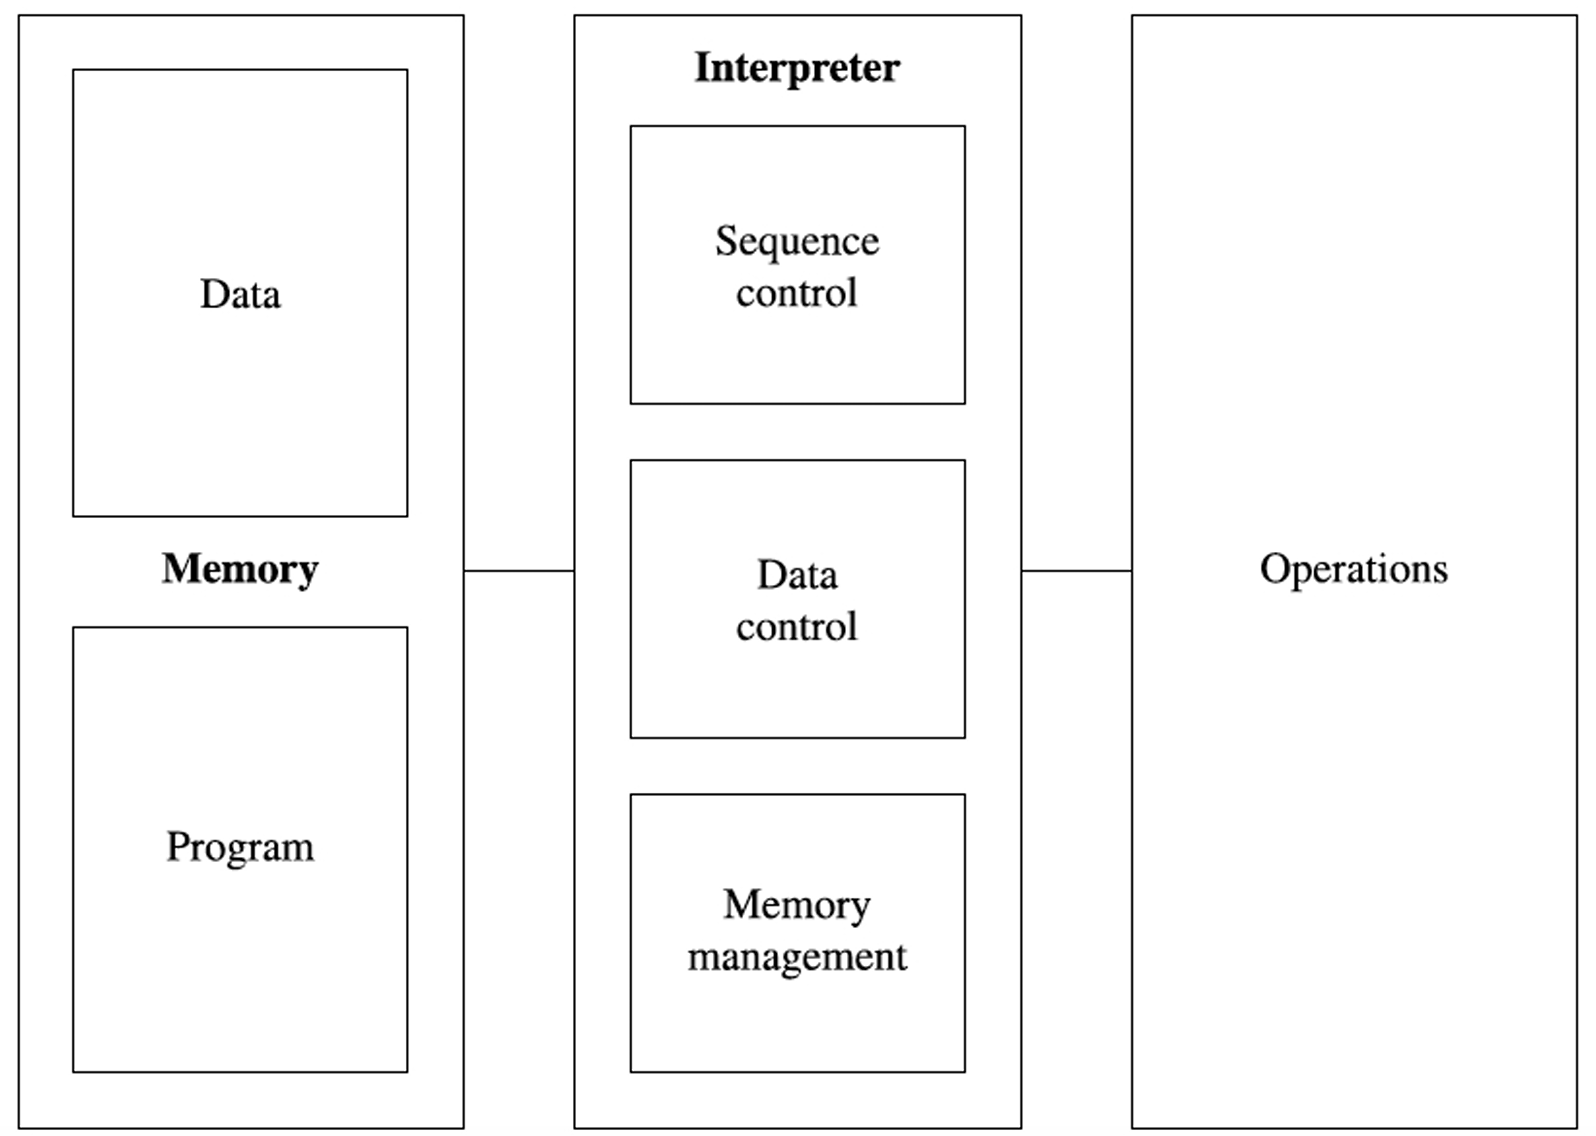
\includegraphics[width=9cm]{img/macchinaAstratta.png}
  \caption{Macchina astratta}
  \label{fig:macchina_astratta}
\end{figure}
Il linguaggio $L$, interpretato dalla macchina $M_L$ viene anche chiamato linguaggio macchina.
Formalmente è l'insieme di tutte le stringhe interpretabili da $M$. Ai componenti 
di $M$ corrispondono opportuni componenti di $L_M$: tipi di dati primitivi 
e costrutti di controllo.

I programmi scritti nel linguaggio macchina di $M$ saranno memorizzati 
nelle strutture dati della memoria della macchina per distinguerli da 
altri dati primitivi su cui opera la macchina. Un esempio di macchina astratta 
è la macchina hardware.

\subsection{Dove realizzare la macchina astratta}
Una qualsiasi macchina per $L$, per essere eseguita, deve prima o poi 
utilizzare qualche dispositivo fisico che concretamente esegue le istruzioni 
di $L$. Questo significa che in qualunque sistema informatico esiste 
sempre una macchina hardware, ma non significa che tutte le macchine 
sono realizzate a livello hardware,  anzi, per poter controllare 
la complessità di un sistema informatico, la realizzazione della macchina 
astratta può avvenire a vari livelli, generalmente sovrapposti, a partire  
da quello fisico. Quindi le macchine astratte possono essere realizzate 
a diversi livelli:
\begin{enumerate}
  \item Hardware: sempre possibile e concettualmente semplice. Si 
  realizza mediante dispositivi fisici, e il linguaggio macchina è il 
  linguaggio binario. L'esecuzione è veloce, ma i programmi ad alto 
  livello sono molto lontani dalle funzionalità elementari a basso livello.
  Inoltre è difficile da modificare, viene usata per sistemi dedicati.
  \item Firmware: Consiste nella simulazione delle strutture dati e degli algoritmi 
  in $M$ mediante microprogrammi. Il linguaggio macchina microprogrammato 
  è a basso livello e consiste ddi microistruzioni che specificano 
  semplici operazioni di trasferimento dati tra registri, da e per la 
  memoria principale ed eventualmente attraverso circuiti logici che 
  realizzano operazioni aritmetiche. I microprogrammi risiedono in speciali 
  aree di memoria di sola lettura. Veloce e più flessibile della realizzazione 
  hardware.
  \item Software: realizzare delle strutture dati e degli algoritmi di $M$ 
  mediante programmi scritti in un altro linguaggio $L'$ che possiamo supporre già 
  implementato. Ovvero, avendo la macchina astratta per $L'$, possiamo realizzare quella per $L$
  mediante opportuni programmi scritti in $L'$ che interpretano i costrutti di $L$ 
  simulando le funzionalità di $M$ per $L$. Riduce la velocità, ma 
  aumenta la flessibilità.
\end{enumerate}
\subsection{Livelli di astrazione}
Per permettere l'uso di linguaggi di programmazione ad alto livello,
controllando la complessità della macchina fisica e del suo vero linguaggio,
quello binario, ai sistemi software è stata data una struttura suddivisa 
a livelli di astrazione cooperanti ma sequenziali e indipendenti:
ciascun livello è definito da un linguaggio $L$ che è l'insieme delle istruzioni 
che il livello mette a disposizione per i livelli successivi/superiori.
Tutte le istruzioni di un linguaggio ad un livello $i-esimo$ sono 
implementate da programmi a livello $j<i$.
\subsection{Come realizzare la macchina astratta}
Per implementare un linguaggio $L$ dobbiamo realizzare una macchina astratta $M_L$, 
in grado di eseguirlo. $M_L$ è quindi un dispositivo che permette di eseguire programmi 
scritti in $L$, ma la corrispondenza non è biunivoca: una macchina astratta corrisponde univocamente 
ad un linguaggio, il suo linguaggio macchina, ma dato un linguaggio $L$ 
esistono infinite macchine astratte che hanno come linguaggio macchina 
esattamente $L$. Tali macchine differiscono nel modo in cui la macchina astratta viene realizzata 
e nelle strutture dati utilizzate. La realizzazione della macchina astratta 
dipenderà quindi dalle funzionalità che le sono messa a disposizione 
dai livelli sottostanti (\textit{tranne il livello hardware}).

Quindi abbiamo un linguaggio $L$ da implementare e una macchina astratta $M_{L_0}$ a disposizione, che 
è macchina ospite. $M_{L_0}$ è il livello su cui vogliamo implementare $L$ e che mette a disposizione 
di $M_L$ le sue funzionalità.

Realizzare $M_L$ consiste quindi in realizzare una macchina che "traduce"
$L$ in $L_0$, ovvero che interpreta tutte le istruzioni di $L$ come sequenza di 
istruzioni di $L_0$. Possiamo quindi distinguere due modalità radicalmente 
diverse a seconda del fatto che si abbia una traduzione "implicita" realizzata 
dalla simulazione dei costrutti di $M_L$ mediante programmi scritti in $L_0$ 
(\textbf{soluzione interpretativa}), oppure si abbia una traduzione "esplicita" dei 
programmi di $L$ in corrispondenti programmi di $L_0$ (\textbf{soluzione compilativa}).
\subsection{Interprete}
Un interprete è un programma $int^{L_0,L}$ che esegue, sulla macchina astratta per $L_0$,
programmi $P^L$, scritti in $L$, su un fissato input $in\in D$. In 
altre parole, un interprete è una \textbf{macchina universale} che 
per un programma e un suo input, lo esegue su quell'input, usando solo funzionalità 
messe a disposizione dal livello sottostante.
\begin{tcolorbox}[title={Interprete da $L$ a $L_0$}]
Dato $P^L \in Pgro^L$ e $in \in D$, un interprete $int^{L,L_0}$ per 
$L$ su $L_0$ è un programma tale che 
$\llbracket int^{L,L_0}\rrbracket:(Prog^L x D)\rightarrow D$ e 
\[
\llbracket int^{L,L^0} \rrbracket (P^L, in) = \llbracket P^L\rrbracket(in)
\]
\end{tcolorbox}
Si osserva che un problema è di fatto una sequenza di istruzioni 
rappresentate da simboli. Questo significa che anche ad alto livello 
può essere assimilato al concetto di dato, e quindi può essere passato come input.
\begin{figure}[H]
  \centering
  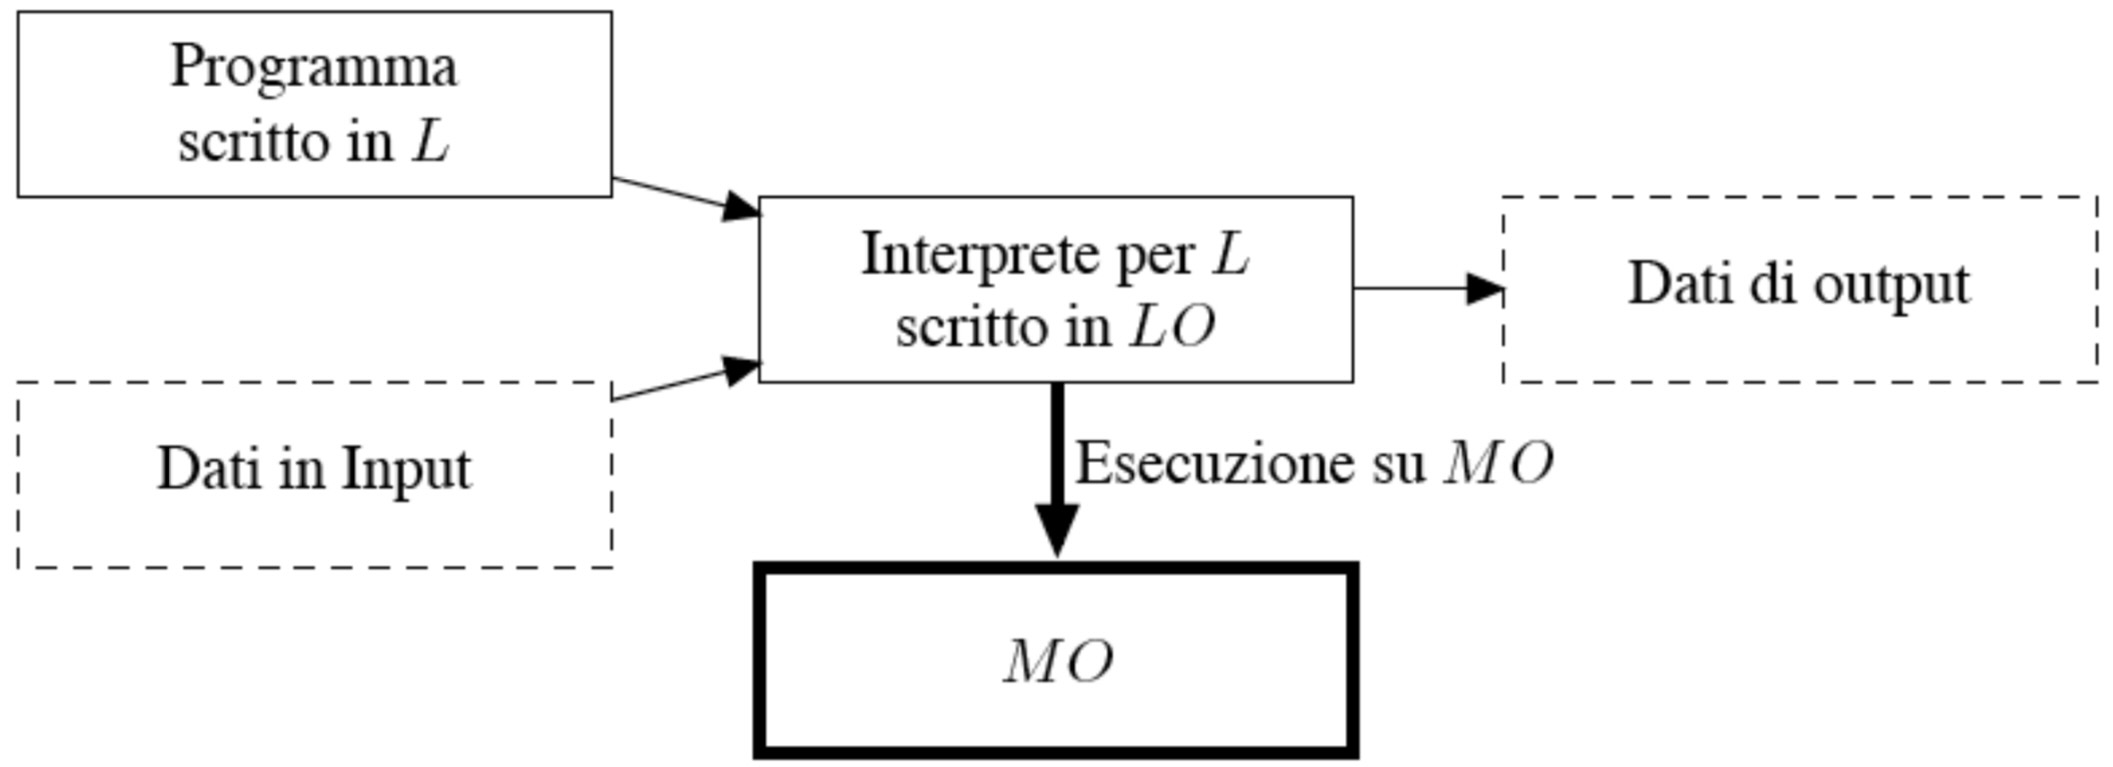
\includegraphics[width=9cm]{img/interprete.jpeg}
  \caption{Soluzione interpretativa}
  \label{fig:int}
\end{figure}
In questo caso non abbiamo una traduzione esplicita, ma solo un percorso 
di decodifica. L'interprete esegue ogni istruzione di $L$ simulandola usando 
un certo insieme di istruzioni di $L_0$. Questa non è una vera traduzione 
in quanto il codice in $L_0$ viene direttamente eseguito, e non 
prodotto in output. Di recente con i linguaggi di scripting, la 
soluzione puramente interpretativa è ritornata in uso.
\subsubsection{Operazioni}
Esattamente come abbiamo visto nell'architettura di Von Neumann, 
un interprete è di fatto un ciclo che attraverso una serie di operazioni 
e funzionalità esegue per simulazione le istruzioni del linguaggio. Tali operazioni sono:
\begin{itemize}
  \item \textbf{Elaborazione dei dati primitivi}: i dati primitivi sono 
  dati rappresentabili in modo diretto nella memoria, ad esempio un macchina 
  fisica i numeri sono dati primitivi. Le operazioni aritmetiche per 
  elaborare questi dati sono direttamente implementate nella struttura della 
  macchina (\textit{operazioni primitive}).
  \item \textbf{Controllo di sequenza delle esecuzioni}: consiste nella gestione 
  del flusso di esecuzione delle istruzioni, non sempre sequenziale. L'interprete 
  dispone infatti di adeguate strutture dati (\textit{ad esempio per 
  memorizzare l'indirizzo della prossima istruzione da eseguire}) che sono manipolate 
  con operazioni specifiche (\textit{ad esempio aggiornamento dell'indirizzo}).
  \item \textbf{Controllo dei dati}: per eseguire le istruzioni è, in 
  generale, necessario recuperare i dati necessari, mediante l'utilizzo anche 
  di strutture ausiliarie. Servono per controllare gli operandi e, in 
  generale, i dati che devono essere trasferiti dalla memoria all'interprete 
  e viceversa. riguardano le modalità di indirizzamento della memoria o l'ordine con sui 
  recuperare gli operandi. A volte necessitano di strutture ausiliarie.
  \item \textbf{Controllo della memoria}: sia il programma che i dati vanno memorizzati nella macchina,
  quindi è necessario gestire processi di allocazione della memoria per i dati e 
  programmi. Nel caso di macchine astratte vicino all'hardware la gestione è abbastanza 
  semplice. Nel caso limite della macchina fisica i dati potrebbero 
  restare sempre nelle stesse locazioni. Nelle macchine astratte software, invece, esistono 
  costrutti di allocazione e deallocazione di memoria che richiedono opportune strutture dati
  (\textit{pile}) e operazioni dinamiche.
\end{itemize}
\subsubsection{Struttura}
Stabilite le operazioni di cui un interprete ha bisogno, vediamo come 
concretamente opera. Il ciclo di esecuzione comune a tutti gli interpreti è:
\begin{lstlisting}
begin
  go := true;
  while go do begin
    FETCH( OPCODE, OPINFO ) at PC 
    DECODE( OPCODE, OPINFO )
    if OPCODE needs ARGS then FETCH( ARGS )
    case OPCODE of 
      OP1: EXECUTE( OP1, ARGS )
      ... 
      OPn: EXECUTE( OPn, ARGS )
      HLT: go := false;
    if OPCODE has result then STORE( RES );
    PC := PC + SIZE( OPCODE );
  end
end
\end{lstlisting}
\begin{enumerate}
  \item Acquisizione prossima istruzione da eseguire.
  \item Decodifica dell'istruzione per estrarre operazioni e operandi
  \item Prelievo dalla memoria degli operandi nel numero richiesto e
  nelle modalità individuate.
  \item Esecuzione dell'operazione.
  \item Memorizzazione dell'eventuale risultato in memoria.
  \item Ripetizione fino al raggiungimento di una operazione di \verb|halt|,
  se raggiungibile.
\end{enumerate}
\subsection{Compilatore}
Un compilatore è un programma $comp^{L_0, L}$, che traduce programmi 
scritti in $L$ in programmi scritti in $L_0$, e quindi eseguibili 
direttamente sulla macchina astratta per $L_0$. Esattamente 
come per l'interprete, anche per il compilatore, un programma può essere assimilato 
al concetto di dato, e quindi passato come input.
\begin{tcolorbox}[title={Compilatore da $L$ a $L_0$}]
Dato $P^L \in Prog^L$, un compilatore $comp^{L,L_0}$ da $L$
a $L_0$ è un programma tale che $\llbracket comp^{L,L_0} \rrbracket:
Prog^L \rightarrow Prog^{L_0}$ e 
\[
\llbracket comp^{L,L_0}\rrbracket (P^L) = P^{L_0}\,\text{tale che}\,
\]
\[
\forall in \in D.\llbracket P^{L_0}\rrbracket (in) =
\llbracket P^{L}\rrbracket(in)
\]
\end{tcolorbox}
In questo caso abbiamo una traduzione esplicita, in quanto il 
codice in $L$ viene prodotto come output e non eseguito.
Quindi, per poter eseguire il programma $P^L$ con input $in$
dovremmo per prima cosa eseguire $comp^{L,L_0}$ con $P^L$
come input. Questa esecuzione avverrà sulla macchina astratta $M_A$
del linguaggio in cui è scritto il compilatore. Questo produce 
come risultato un altro programma (\textit{compilato}) $P^{L_0}$.
A questo punto possiamo eseguire $P^{L_0}$ su $M_{L_0}$ con 
input $in$. Molti linguaggi imperativi ad alto livello sono compilati.
\subsubsection{Struttura}
La compilazione dove tradurre un programma da un linguaggio 
ad un altro preservandone la semantica:
dobbiamo avere la certezza che il programma compilato faccia
esattamente quello che faceva il programma originale/sorgente.
Per questo un compilatore è uno strumento più difficile da progettare 
rispetto all'interprete. L'esecuzione di un compilatore passa 
attraverso varie fasi:
\begin{itemize}
  \item \textbf{Analisi lessicale (Scanner)}: spezza un programma 
  nei componenti sintattici primitivi, chiamati \textbf{token}. 
  I token formano linguaggi regolari.
  \item \textbf{Analisi sintattica (Parser)}: crea una rappresentazione 
  ad albero della sintassi del programma dove ogni foglia 
  è un token e le foglie lette da sinistra a destra costruiscono 
  frasi ben formate del linguaggio. Tale albero costituisce la 
  struttura logica del programma, quando non è possibile costruire 
  l'albero significa che qualche frase è illegale. In 
  tal caso la compilazione si blocca con un errore. Le frasi 
  di token formano linguaggi CF.
\end{itemize}
\subsubsection{Interprete o compilatore?}
Entrambe le soluzioni, nella loro forma pura hanno vantaggi 
e svantaggi:
\begin{itemize}
  \item implementazione \textbf{interpretativa} pura: interpreta 
  al momento dell'esecuzione, permette di interagire in modo diretto con l'esecuzione 
  del programma (\textit{importante nel debugging}). Un interprete 
  è più veloce da sviluppare rispetto ad un compilatore ed usa 
  meno memoria. D'altra parte i tempi di decodifica si sommano
  a quelli di esecuzione, ogni volta che una certa istruzione 
  viene eseguita.
  \item implementazione \textbf{compilativa} pura: trascurando 
  i tempi di compilazione, l'esecuzione del programma è più efficiente 
  anche perché nella fase di compilazione il codice viene, in generale,
  ottimizzato. L'interazione è invece più difficile. Un errore 
  a runtime è difficile da associare all'esatto comando del codice 
  sorgente che lo ha generato, per questo il debugging è più 
  difficile.
\end{itemize}
\subsection{Soluzione ibrida}
Esiste un compromesso tra compilatore e interprete, ovvero una soluzione 
ibrida dove il linguaggio ad alto livello viene compilato 
in un linguaggio a più basso livello che poi viene interpretato. 
In questo caso, consideriamo il linguaggio $L$, ad alto livello, per 
il quale dobbiamo realizzare la macchina astratta $M_L$. $L$ viene quindi 
tradotto in un linguaggio intermedio $L_{M_I}$ la cui macchina 
astratta $M_I$ consiste in un interprete del linguaggio $L_{M_I}$
sulla macchina ospite $M_O$.
\chapter{Descrivere i linguaggi}
Un linguaggio di programmazione è un formalismo artificiale 
mediante il quale esprimono algoritmi. Anche se artificiale, è sempre 
un linguaggio e quindi deve essere descritto usando noti strumenti 
della linguistica.

Un linguaggio di programmazione non è altro che un linguaggio naturale, ma 
semplificato e non ambiguo. La teoria dei linguaggi di programmazione 
quindi deve parlare di:
\begin{itemize}
  \item Grammatica (\textit{sintassi}): regole di formazione, la correttezza della 
  frase (\textit{relazioni tra segni}).
  \item Semantica: attribuzione di significato: associare un significato ad una 
  frase corretta.
  \item Pragmatica: in quale modo le frasi corrette e sensate sono usate.
  \item Implementazione: eseguire una frase corretta, rispettando 
  la semantica.
\end{itemize}
Semantica, pragmatica e implementazione sono elementi da studiare separatamente 
ma legati dalla sintassi in funzione della quale tutti sono definiti.
\section{Descrivere i linguaggi di programmazione}
La descrizione di un linguaggio di programmazione avviene su tre 
dimensioni (\textit{Morris, 1939}):
\begin{itemize}
  \item \textbf{Sintassi}: è l'insieme di regole che permettono di 
  costruire frasi corrette. Ogni frase è costruita da componenti 
  che rappresentano le categorie sintattiche. Dopo di che, 
  individuato l'alfabeto, a livello lessicale si individuano le sequenze 
  di simboli legali, ovvero quelle che costruiscono le parole del linguaggio.
  La fase che determina la corretta struttura delle frasi, ovvero 
  che verifica se una frase rispetta le regole della grammatica, è detta \textit{parsing}.
  \item \textbf{Semantica}: nei linguaggi artificiali l'attribuzione del 
  significato è una fase semplice ed è la definizione di una relazione 
  tra segni e significati. Ad esempio, la semantica di un programma 
  può essere la funzione matematica calcolata dal programma. Solitamente 
  viene specificata descrivendo gli effetti della sintassi su una 
  rappresentazione astratta della macchina, chiamato \textit{stato}.
  \item \textbf{Pragmatica}: frasi con lo stesso significato possono essere 
  usate in modo diverso in modo dipendente dal contesto linguistico.
  \item \textbf{Implementazione}: questi aspetti riguardano la tecnica 
  di implementazione usata.
\end{itemize}
\subsection{Sintassi}
Le regole sintattiche del linguaggio specificano quali stringhe 
di caratteri sono legali nel linguaggio. Nel dettaglio la terminologia 
nella linguistica è la seguente:
\begin{itemize}
  \item Una \textit{parola} è una stringa di caratteri su un alfabeto.
  \item Una \textit{frase} è una sequenza (\textit{ben formata}) di parole.
  \item Un \textit{linguaggio} è un insieme di frasi.
\end{itemize}
Nell'ambito dei linguaggi di programmazione gli stessi concetti 
prendono nomi differenti:
\begin{itemize}
  \item Le parole diventano \textit{lessemi}. Un lessema è una 
  parola con significato specifico, nella grammatica corrisponde ad un terminale.
  È l'unità minima sintattica, ovvero quella a più basso livello di un linguaggio 
  di programmazione (\textit{ad esempio:} \verb|*|, \verb|sum|, \verb|begin|,\dots). La 
  loro specifica sintattica è separata dalla definizione del linguaggio, e come vedremo,
  solitamente descritta come stringhe di linguaggi regolari.
  \item Le frasi diventano \textit{token}. I token corrispondono 
  agli elementi delle categorie sintattiche del linguaggio di programmazione, 
  e nella grammatica corrispondono alle sequenze generate dai simboli 
  non terminali.
  \item Il \textit{programma} è una sequenza/composizione sequenziale 
  di frasi ben formate.
  \item Il linguaggio dei programmi, e quindi gli strumenti formali 
  che lo definiscono, costituiscono quello che chiamiamo \textit{linguaggio 
  di programmazione}.
\end{itemize}
\subsubsection{Descrivere la sintassi}
Abbiamo bisogno di strumenti formali per descrivere parole 
e frasi legali di un linguaggio, che permettano in modo automatico 
di verificare l'appartenenza o meno al linguaggio. In particolare, 
le parole sono stringhe di simboli alfabetici, mentre le frasi sono stringhe di 
parole.

Nei linguaggi di programmazione, il linguaggio dei lessemi 
è in generale sempre un linguaggio \textbf{regolare}, quindi 
\textbf{riconoscibile} da un automa a stati finiti.
\begin{tcolorbox}[title={Riconoscitore}]
Si tratta di uno strumento di riconoscimento che legge in 
input stringhe sull'alfabeto del linguaggio e decide se la 
stringa appartiene o meno al linguaggio.
\end{tcolorbox}
Supponiamo di avere un linguaggio $L$ su un alfabeto $\Sigma$, per 
costruire un metodo di riconoscimento dovremmo avere un meccanismo 
$R$ in grado di leggere le stringhe di caratteri. $R$ quindi deve essere in 
grado di dire se una stringa è in $L$ oppure no.

Invece, il linguaggio di token, e quindi dei programmi, è in generale
un linguaggio \textbf{context-free (CF)}, quindi \textbf{generato} da 
una grammatica CF.
\begin{tcolorbox}[title={Generatore}]
Si tratta di uno strumento che genera stringhe di un linguaggio. 
Si può determinare se la sintassi di una particolare
frase è sintatticamente corretta confrontandola con la struttura 
del generatore (\textit{parser}).
\end{tcolorbox}
Possiamo comunque osservare che anche i linguaggi regolari possono essere 
generati (\textit{grammatiche regolari}) e i linguaggi 
CF possono essere riconosciuti (\textit{automi a pila}).
\subsubsection{Esempio}
\[
\mathcal{L}=\{\sigma \in \Sigma^* \mid |\sigma|\, pari \}\qquad\Sigma=\{a,b\}
\]
\begin{figure}[H]
  \begin{center}
    \begin{tikzpicture}[shorten >=1pt,node distance=4cm,on grid]
      \node[state, accepting] (q0) {$q_0$};
      \node[state] (qbot) [right=of q0] {$q_\bot$};
      \path[->]
        (q0) edge [bend left] node [above] {a,b} (qbot)
        (qbot) edge [bend left] node [below] {a,b} (q0);
    \end{tikzpicture}
  \end{center}
\end{figure}
\[
\mathcal{S} \longrightarrow \varepsilon \mid aa\mathcal{S} \mid bb\mathcal{S} \mid ab\mathcal{S} \mid ba\mathcal{S}
\]
Ma vediamo quali sono questi strumenti formali, in particolare 
per descrivere il linguaggio come sequenza di parole/lessemi.
Come si descrive quindi la sintassi? Nel linguaggio naturale 
viene usato il linguaggio naturale stesso, ma il linguaggio naturale 
introduce ambiguità e non può essere di aiuto all'implementazione di 
un linguaggio di programmazione. Negli anni '50, Chomsky ha 
sviluppato un formalismo al fine di descrivere i linguaggi artificiali in 
modo formale, permettendo di limitare le ambiguità: \textbf{grammatiche 
generative}, molto utilizzate per descrivere la sintassi dei linguaggi di 
programmazione.

Il vocabolario è alla base per costruire un dizionario completo 
delle parole del linguaggio. La grammatica descrive i modi per 
combinare parole e formare frasi, ed è descritta da:
\begin{itemize}
  \item \textit{Alfabeto}.
  \item \textit{Descrizione lessicale}: sequenze di simboli 
  corretti che costituiscono \textbf{parole/lessemi} del linguaggio.
  \item Descrizione delle \textit{sequenze di parole} che costituiscono 
  frasi legali del linguaggio.
\end{itemize}
\subsubsection{Esempio}
\[
\mathcal{L}= \{\sigma \in \Sigma^* \mid \sigma\,palindrome\}
\]
\textit{Definizioni}: 
\begin{itemize}
  \item $\varepsilon$, $a$ e $b$ sono palindromi.
  \item se $\sigma$ è palindrome allora lo sono anche $a\sigma a$ e $b\sigma b$
\end{itemize}
\[
\mathcal{S} \longrightarrow \varepsilon \mid a \mid b \mid a\mathcal{S} a \mid b\mathcal{S} b
\]
\subsection{Grammatiche context-free}
\begin{tcolorbox}
Una grammatica libera dal contesto (CF) è un quadrupla $\mathcal{G} = 
\langle \mathcal{V}, \mathcal{T}, \mathcal{P}, \mathcal{S} \rangle$, ove:
\begin{itemize}
  \item $\mathcal{V}$ è un insieme finito di variabili (detta anche simboli \textit{non terminali}),
  \item $\mathcal{T}$ è un insieme finito di simboli \textit{terminali} ($\mathcal{V}\cap \mathcal{T} = \varnothing$),
  \item $\mathcal{P}$ è un insieme finito di produzioni; ogni produzione 
  è della forma $\mathcal{A}\rightarrow \alpha$, ove:
  \begin{itemize}
    \item $\mathcal{A} \in \mathcal{V}$ è una variabile, e 
    \item $\alpha \in (\mathcal{V} \cup \mathcal{T})^*$
  \end{itemize}
  \item $\mathcal{S}\in \mathcal{V}$ è una variabile speciale, detta \textit{simbolo iniziale}.
\end{itemize}
\end{tcolorbox}
Nella grammatica i simboli terminali costituiscono
parole/lessemi del nostro linguaggio, ovvero il
vocabolario, invece i simboli non terminali sono le
categorie sintattiche, quindi rappresentano i diversi tipi di
elementi che possono essere usati per comporre frasi. Le
produzioni sono le regole di composizione degli elementi
in una frase, formalmente sono utilizzate per rimpiazzare
un non terminale con una stringa di uno o più simboli terminali 
e/o non terminali. Il linguaggio è l'insieme di tutte le possibili frasi,
ovvero le stringhe di simboli terminali, generate a partire 
dal simbolo iniziale $\mathcal{S}$, che rappresenta la categoria delle 
frasi legali nel linguaggio.

Ma cosa significa context free? Significa \textbf{libero dal contesto}, 
questo è un vincolo sulle produzioni, dove a sinistra possiamo 
trovare un solo non terminale, e questo implica che in una frase, 
dovunque troviamo quel non terminale, ovvero \textbf{qualunque contesto} 
troviamo quel non terminale, lo possiamo sostituire applicando 
una delle produzioni per il non terminale.
Nei linguaggi di programmazione, questo significa che il modo con cui possiamo 
sviluppare, per sostituzione, una categoria sintattica è indipendente dal contesto.

Questo è un vantaggio perché dato un programma, abbiamo il problema di capire 
quale grammatica può averlo generato (\textit{parsing}), e per le grammatiche 
CF esistono strumenti automatici efficienti di parsing. Dal punto di vista 
della complessità del parsing, questa dipende dal numero di simboli terminali della 
grammatica e in grado di non determinismo delle produzioni. Un linguaggio 
può essere generato da diverse grammatiche, quindi ai fini dell'efficienza 
del linguaggio è importante come si sceglie la grammatica. Per prima cosa 
deve essere semplice, il più semplice possibile: CF, basso non determinismo, 
deve facilitare la definizione semantica del linguaggio (\textit{ad esempio 
grammatiche lineari destre}).

Purtroppo, la proprietà CF è anche uno svantaggio per i linguaggi di programmazione,
infatti tali grammatiche non riescono a catturare i vincoli contestuali, che 
pure sono necessari: Ad esempio il poter usare una variabile solo se 
questa è stata dichiarata precedentemente. Questo, significa che abbiamo bisogno 
di altri formalismi per descrivere/verificare questa tipologia di vincoli 
su cui ritorneremo.
\subsubsection{Esempio}
\[
\mathcal{G}=\{\{\mathcal{E}\},\{or,and,not,(,),0,1\}, \mathcal{P}, \mathcal{E}\}
\]
\[
\mathcal{E}=0\mid 1 \mid (\mathcal{E}\,or\,\mathcal{E})\mid (\mathcal{E} \,and\,\mathcal{E})\mid 
(not\, \mathcal{E}).
\]
\[
\begin{matrix}
  \mathcal{E} & \longrightarrow & 0 \\
  \mathcal{E} & \longrightarrow & 1 \\
  \mathcal{E} & \longrightarrow & (\mathcal{E}\,or\,\mathcal{E}) \\
  \mathcal{E} & \longrightarrow & (\mathcal{E}\,and\,\mathcal{E}) \\
  \mathcal{E} & \longrightarrow & (not\,\mathcal{E})
\end{matrix}
\]
\subsection{Descrivere un semplice linguaggio}
Un linguaggio può essere descritto anche in modo informale, descrivendo 
quali caratteristiche vogliamo inserire e quale è il loro significato:
\begin{itemize}
  \item Niente dichiarazioni.
  \item Solo variabili ed espressioni booleane.
  \item Assegnamento e composizione sequenziale.
  \item Comando condizionale.
  \item Comando iterativo (\textit{loop}).
\end{itemize}
Questo può essere sufficiente per scrivere un programma corretto che un altro 
programmatore può leggere, ma non è adeguato per costruire un compilatore o 
un interprete. Per permettere l'implementazione della macchina astratta abbiamo 
bisogno di scendere ad un livello più formale.

Ritorna il concetto di astrazione, ed in particolare osserviamo che ogni 
linguaggio è descritto a più livelli di astrazione, ognuno descritto da una 
grammatica.
\begin{figure}[H]
  \centering
  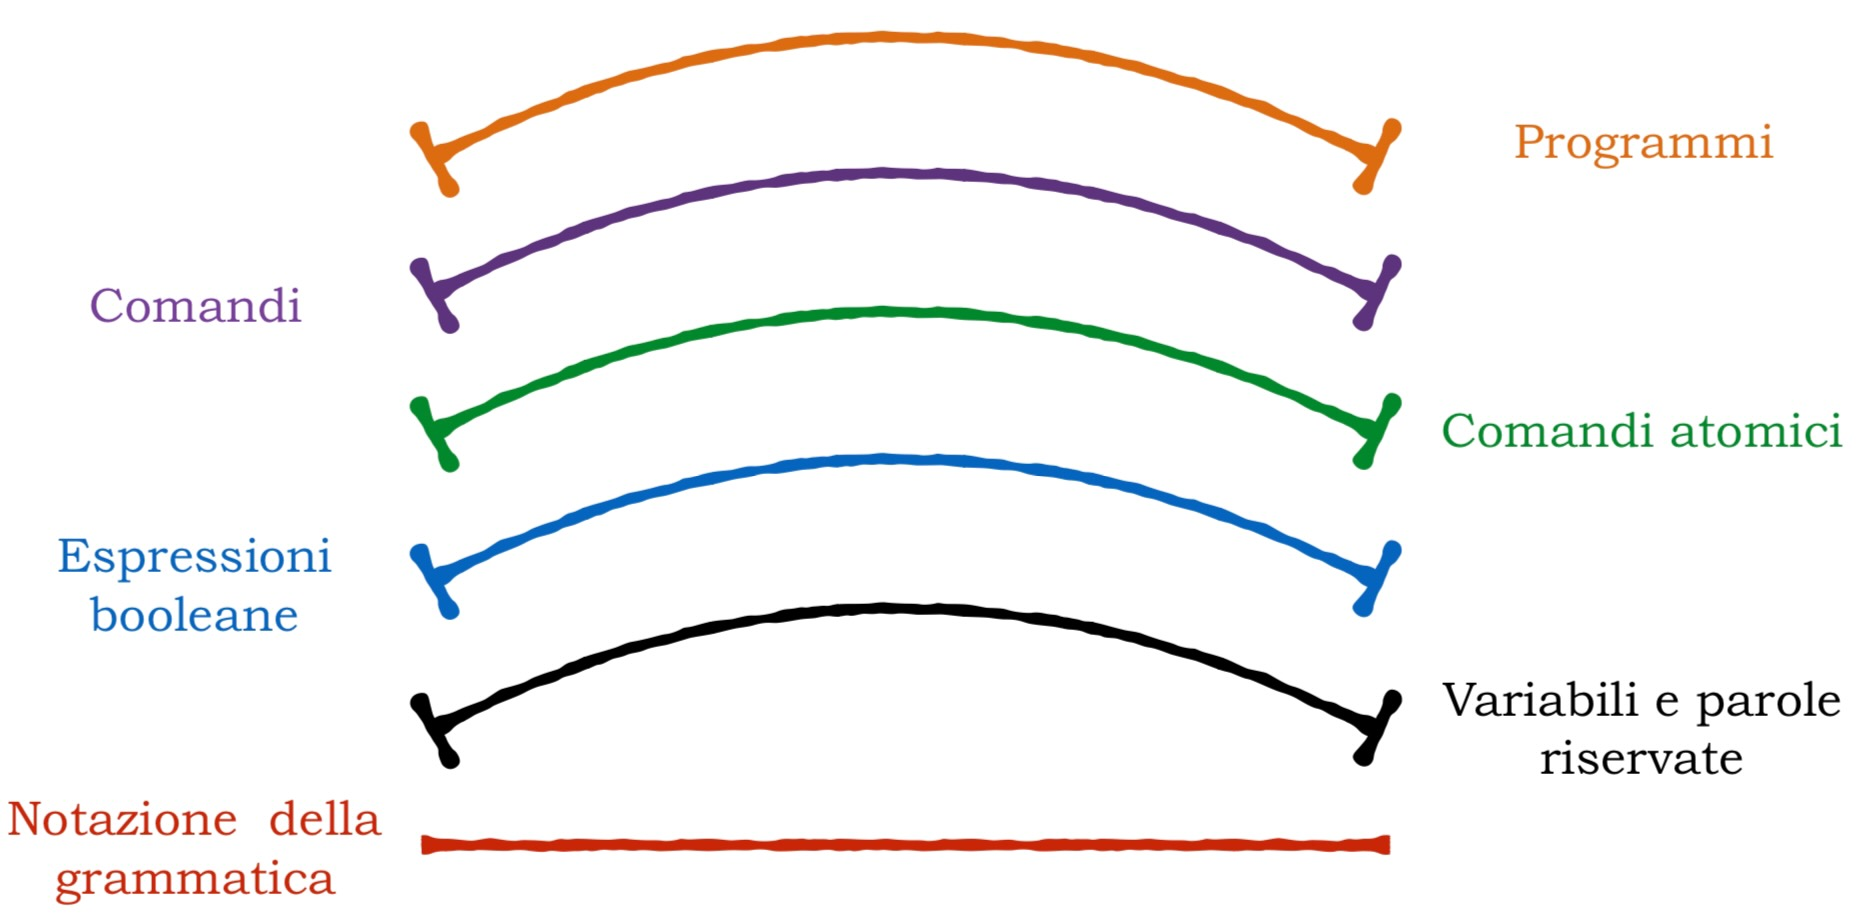
\includegraphics[width=9cm]{img/imperativo.jpeg}
  \label{fig:esempiolingimperativo}
\end{figure}
\begin{figure}[H]
  \centering
  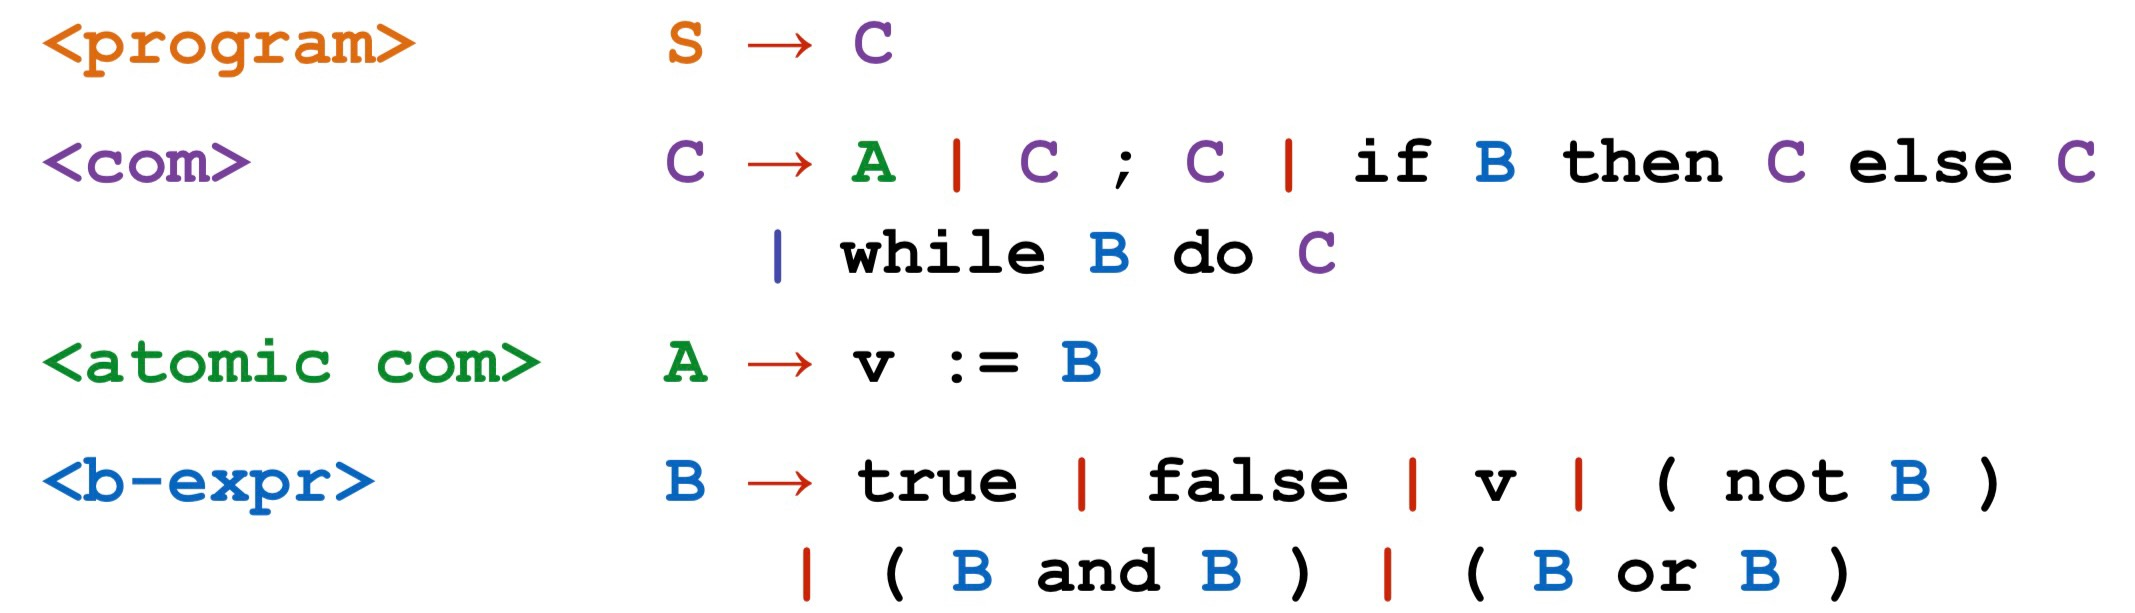
\includegraphics[width=9cm]{img/linguaggioEx.jpeg}
  \label{fig:linguaggioEx}
\end{figure}
Le frasi del linguaggio sono i programmi, niente dichiarazioni 
e niente preamboli. Un programma è qualunque comando e ogni comando è 
qualunque programma. Ad ogni livello di specifica della grammatica 
quanto specificato alle grammatiche sottostanti è trattato da terminale, ma per 
avere una definizione completa dobbiamo necessariamente definire esplicitamente 
anche questi livelli. Quindi, ad esempio, nella grammatica dei comandi $(C)$ 
usiamo la categoria sintattica dei comandi atomici $(A)$, questo significa 
che ogni frase generata da $A$ è trattata come un terminale della grammatica 
per $C$.
Analogo per le espressioni di booleane $(B)$.

Nelle espressioni abbiamo una notazione completamente "parentesizzata" 
per evitare ambiguità, se togliamo le parentesi introduciamo ambiguità.
L'ambiguità consiste nell'esistenza di più parse-tree per la stessa espressione.

Chiaramente l'ambiguità è da evitare perché vogliamo che ogni costrutto abbia 
un significato unico. In ogni caso le grammatiche sono ambigue per semplificare la 
rappresentazione assumendo implicitamente le convenzioni ereditate dalla matematica.
In questo linguaggio ci sono ambiguità anche nei comandi, ad esempio nella composizione sequenziale.

\subsection{Analisi semantica}
Ritornando ai limiti del formalismo che usiamo per descrivere i linguaggi di 
programmazione, ovvero l'essere CF. Abbiamo già osservato che ci siano vincoli 
che dipendono dal contesto:
\begin{itemize}
  \item Il numero di parametri attuali di una chiamata di procedura deve essere 
  uguale al numero dei parametri formali della dichiarazione.
  \item Un'operazione sintatticamente corretta potrebbe essere illegale in 
  cui si trova ($i := r + 3$). Se il linguaggio è fortemente tipato e prima non 
  ci fosse una dichiarazione di $r$ e di $i$, il comando sarebbe illegale.
  \item I tipi della variabile e dell'espressione di un assegnamento devono 
  essere compatibili.
\end{itemize}
Quindi stringhe corrette per una certa grammatica sono legali solo in 
determinati contesti. Questo è chiaramente un vincolo sintattico, ma lo strumento
sintattico scelto non permette di descriverlo.

Possiamo percorrere diverse strade per risolvere la questione:
\begin{itemize}
  \item Usare strumenti più potenti, per esempio grammatiche contestuali:
  riscrittura di un non-terminale solo in un determinato contesto.
  \item Usare controlli ad hoc.
\end{itemize}
Il problema delle grammatiche contestuali è che non esistono algoritmi lineari per 
il riconoscimento di stringhe generate, quindi non ci sono algoritmi efficienti 
per fare il parser delle stringhe di una grammatica dipendente dal contesto.
Per questo la scelta ricade su una specifica del linguaggio mediante grammatica 
CF (\textit{sintassi}) e poi, come parte semantica (\textit{da cui il nome di 
vincoli semantici o semantica statica}), vengono specificati i vincoli contestuali.
\subsection{Semantica (dinamica)}
La semantica è più complessa della sintassi perché ricerca esattezza e flessibilità.
\begin{itemize}
  \item \textbf{Esattezza}: descrizione precisa e non ambigua di cosa ci si 
  debba aspettare da ogni costrutto sintatticamente corretto, per sapere a priori 
  quello che succederà durante l'esecuzione.
  \item \textbf{Flessibilità}: non deve anticipare scelte che possono essere 
  demandate all'implementazione.
\end{itemize}
Non esiste un singolo formalismo universalmente accettato per dare significato ai 
programmi, ma esistono diverse necessità di metodologia per descrivere significati:
\begin{itemize}
  \item I programmatori devono sapere cosa significano i comandi.
  \item Gli sviluppatori devono sapere esattamente cosa fanno i costrutti.
  \item Gli sviluppatori potrebbero rilevare ambiguità e inconsistenze.
  \item Dimostrazioni di correttezza dovrebbero essere possibili.
  \item Generatori di compilatori dovrebbero essere possibili. 
\end{itemize}
Quella che dobbiamo formalizzare per rispondere a tutte queste problematiche 
è la \textbf{semantica} del linguaggio di programmazione, a volte anche chiamata 
semantica dinamica, per distinguerla da quella statica. Perché serve quindi? 
Dobbiamo specificare gli effetti della sintassi sulla rappresentazione astratta 
della macchina, chiamata \textbf{stato}. Quindi, per ogni costrutto, va descritto 
il significato della sua esecuzione come trasformazione di stato. L'astrazione della 
macchina nel concetto di stato permette di dare al costrutto un significato puro, indipendente 
dalla macchina, quindi senza restrizioni.
\begin{tcolorbox}[title={Semantica}]
La semantica attribuisce significato ad ogni frase sintatticamente corretta.
\end{tcolorbox}
\begin{tcolorbox}[title={Siginficati}]
I significati sono entità autonome che esistono indipendentemente dai segni 
che usiamo per descriverle.
\end{tcolorbox}
La semantica guarda quindi al linguaggio di programmazione ad un livello ideale, indipendente
dalla macchina, con l'unico vincolo che in ogni istante possono essere eseguiti un numero finito di passi di 
computazione. Chiaramente, non è facile trovare il giusto equilibrio tra esattezza e flessibilità, 
in modo da rimuovere ambiguità, ma anche lasciare spazio all'implementazione.

Come possiamo quindi dare significato ad un linguaggio di programmazione? Di certo non possiamo dare un significato esplicito 
ad ogni frase del linguaggio essendo queste infinite, quindi anche la semantica 
deve fornire una rappresentazione finita del significato dei programmi a partire dalla sua 
sintassi.
Abbiamo visto che la sintassi è descritta attraverso un vocabolario (\textit{di elementi primitivi}) e
un insieme di regole per combinare le parole del vocabolario (\textit{produzioni che combinano categorie sintattiche
in una frase e le istanziano nelle parole del vocabolario}). 
Anche la semantica quindi, per essere descritta in modo finitario,
pur dando significato ad un insieme infinito deve basarsi sulla struttura
costruttiva della sintassi. Deve dare
semantica agli elementi primitivi e deve descrivere il
significato di una forma composta in funzione del significato
degli elementi composti. Quindi in generale il significato di un
programma è la composizione del significato dei costrutti che lo compongono.
Il significato di ogni costrutto è dato in termini del significato delle categorie
sintattiche e quindi delle parole che lo compongono, e così via fino ad arrivare
ad usare il significato di un vocabolario finito e noto. In sintesi,
quindi per dare semantica dobbiamo sempre dare significato agli elementi
complessi in funzione del significato degli elementi più semplici che lo compongono e
del modo con cui questi sono composti.

Esiste quindi un legame forte tra sintassi e semantica: sintassi
come metodo finitario per rappresentare un insieme infinito
di programmi, la cui sola cosa analizzabile è la struttura;
semantica come metodo finitario (\textit{per questo dato seguendo
la struttura della sintassi}) per dare significato a tutti gli
elementi dell'insieme infinito dei programmi.
\subsection{Induzione}
Quindi la semantica va data seguendo la struttura della sintassi,
e la sintassi è definita descrivendo gli elementi 
base e componendo questi elementi, attraverso regole,
in elementi composti. Questa forma di definizione ha una
connotazione ben precisa nella matematica, ed è chiamata \textbf{induzione}.
Si usa sempre un ordine ben fondato perché questo garantisce di trovare
sempre un minimo. Ovvero riesco a trovare la base dell’induzione sulla
quale la proprietà è definita direttamente. L'induzione strutturale è usata
per definire/dimostrare proprietà sui linguaggi di programmazione. 
L’idea centrale nell’induzione è quella di avere una base su cui definire/dimostrare
direttamente (\textit{esplicitamente}) la proprietà, e poi avere regole di 
costruzione/definizione che, assumendo definitiva/vera la proprietà degli elementi 
usati, si definisce/dimostra la proprietà per l'elemento del composto. Quindi 
si opera induttivamente sulle regole di costruzione dell'insieme.
\begin{tcolorbox}[title={Induzione matematica e strutturale}]
Dato un insieme A ed una relazione binaria
$< \subseteq A \times A$ ben fondata (\textit{senza catene discendenti infinite}).
Se $A=\mathbb{N}$ si ha induzione matematica
Se $\mathcal{A}=\mathcal{L}(\mathcal{G})$ linguaggio generato
da una grammatica $\mathcal{G}$ si ha induzione strutturale.
\end{tcolorbox}
\begin{tcolorbox}[title={Principio di induzione strutturale}]
Per dimostrare che una proprietà è valida per tutti gli elementi
di una categoria sintattica:
\begin{enumerate}
  \item Si dimostra la proprietà per tutti gli elementi base della
  categoria, quelli che non hanno nessun elemento come componente
  (\textit{base induttiva}).
  \item Si dimostra la proprietà per tutti gli elementi composti
  assumendo che la proprietà sia verificata da tutti i loro componenti
  immediati (\textit{ipotesi induttiva}).
\end{enumerate}
\end{tcolorbox}
\subsubsection{Esempio di induzione matematica}
\begin{proof}[\textbf{Dimostrazione induttiva}]
  Dimostrare che:
  \begin{equation*}
      \sum_{i = 1}^{n} i = \dfrac{n \left( n + 1 \right)}{2} \hspace{2em} \text{con } n \ge 1
  \end{equation*}
  La \textbf{base induttiva} è con $n$ pari ad $1$, quindi sostituendo:
  \begin{equation*}
      n = 1 \hspace{2em} \sum_{i = 1}^{1} i = 1 = \dfrac{1 \left( 1 + 1 \right)}{2}
  \end{equation*}
  Per il \textbf{passo induttivo} si suppone che sia vero per $n$ considerando dunque come passo induttivo l'equazione iniziale. Si dimostra per $n + 1$:
  \begin{equation*}
      \begin{array}{rll}
          \displaystyle\sum_{i=1}^{n+1} i & = & \dfrac{ \left(n+1\right) \left(n+2\right) }{2} \\
          \\
          \displaystyle\sum_{i=1}^{n+1} i \triangleq \underbrace{\sum_{i=1}^{n} i + \left(n+1\right)}_{\text{per definizione}} & = 
          & \underbrace{\dfrac{n \left(n+1\right)}{2}}_{\text{ip. induttiva}} + \: n + 1 \\
          \\
          & = & \dfrac{n \left(n+1\right) + 2n + 2}{2} = \dfrac{n^{2} + n + 2n + 2}{2} \\
          \\
          & = & \dfrac{\left(n+1\right) n + \left(n+1\right) 2}{2} = \dfrac{\left(n+1\right) \left(n+2\right)}{2}
      \end{array}
  \end{equation*}
\end{proof}
\subsection{Un significato tante rappresentazioni}
Abbiamo già parlato del fatto che ogni programma è una
funzione matematica tra domini specifici. In particolare, un
programma è solo una notazione per rappresentare
funzioni. Infatti un algoritmo è una entità astratta
concretizzata in un programma, ma una volta che abbiamo
il programma non ci interessa se il programma implementa
esattamente l’algoritmo, ma ci interessa che il programma
implementi precisamente la funzione descritta
dall'algoritmo. Il fatto che la funzione venga descritta
mediante un algoritmo significa solamente che abbiamo in
mente un modello computazionale che ci permette
di suddividere la funzione in passi computazionali primitivi del modello 
computazionale. 
Quindi l’algoritmo è solo una 
dimensione intermedia che riempie il gap tra la funzione e
il programma. In questo senso una strada è sicuramente
quella di descrivere il significato di un programma
caratterizzando la sua funzionalità. Questo è sicuramente
quello che interessa al progettista che deve progettare i
costrutti del linguaggio per permettere l’implementazione
di certe funzionalità e perché la composizione permetta di
implementare certe funzionalità. D’altra parte
l'implementatore ha sempre bisogno di descrivere
funzionalità ma le deve descrivere come trasformazione di
stato della macchina, fissati gli stati di input quali sono gli
stati di output ottenuti dopo l’esecuzione del costrutto? Dal
punto di vista dello sviluppatore invece non interessa
l’esatta trasformazione di stato, ma interessa come l’uso e
la combinazione dei costrutti permetta di preservare invarianti
o garantire proprietà desiderate.
\begin{itemize}
  \item Comportamento I/O: interessa l'implementatore;
  \item Funzionalità descritta dall'algoritmo: interessa il progettista;
  \item Proprietà - Invarianti: interessa lo sviluppatore.
\end{itemize}
Tutte queste visioni sono necessariamente collegate, nel senso che ogni funzione
è una relazione e quindi una collezione di proprietà e viceversa ad ogni
collezione di proprietà può essere associata una relazione o una funzione.
Di fatto tutte queste rappresentazioni, tutti i punti di vista sono equivalenti,
guardano solo al problema di rappresentare il significato da punti di vista
diversi. I vari punti di vista hanno dato origine a diversi tipi di semantica
che modellano i significati mediante strumenti matematici diversi (\textit{funzioni, 
transizioni di stato, proprietà}). A seconda di quali strumenti matematici usiamo per 
descrivere i significati otteniamo tipi di semantiche diverse rendendo più 
agevoli tipi diversi di ragionamento. Le tipologie di strumenti possono essere 
raccolte in tre macro classi: 
\begin{itemize}
  \item \textbf{Denotazionale} (\textit{descrive funzionalità}): studia gli effetti dell'esecuzione, cerca proprietà 
  del programma studiando proprietà della funzione calcolata.
  \item \textbf{Assiomatica} (\textit{descrive proprietà}): serve per fare deduzioni logiche a partire da 
  assiomi dati, su parti del programma.
  \item \textbf{Operazionale} (\textit{descrive trasformazioni di stato}): si preoccupa di come i risultati finali vengono prodotti.
\end{itemize}
\subsubsection{Esempio}
\begin{lstlisting}
z := 2;
y := z;
y := y + 1;
z := y;
\end{lstlisting}
\subsubsection{Denotazionale}
\begin{tcolorbox}[title = {Semantica denotazionale}]
Modello matematico dei programmi basato sulla ricorsione. È la semantica
più “astratta” con cui descrivere i programmi.
\end{tcolorbox}
Il processo di costruzione della semantica denotazionale
per un linguaggio consiste nel definire un oggetto matematico per ogni entità
del linguaggio e nel definire poi una funzione che mappa istanze delle entità
del linguaggio in istanze dei corrispondenti oggetti matematici. Solitamente,
il significato dei costrutti del linguaggio è definito solo in funzione del
valore delle variabili del programma, ovvero in funzione della rappresentazione
dello stato della macchina.

Formalmente, il modello matematico usato per descrivere la semantica
denotazionale è quello delle funzioni matematiche (\textit{ricorsive}),
ovvero un programma corrisponde ad una funzione tra stati della macchina
e l’equivalenza di programmi si dimostra mediante equivalenza tra funzioni.

Quindi la semantica denotazionale è un oggetto puramente matematico che descrive
gli effetti semplicemente manipolando oggetti matematici (\textit{si astrae da ogni
concetto di esecuzione}). In particolare, guarda agli effetti dell’esecuzione
del programma, descrivendo l’effetto dell’esecuzione di una sequenza di comandi
separati da $;$ attraverso la composizione degli effetti dei singoli comandi da
sinistra verso destra. L’effetto di ogni comando è la funzione che dato uno stato
produce un nuovo stato. 

Questa semantica può essere usata per dimostrare la correttezza dei programmi,
fornisce un modo formale per ragionare sui programmi, può aiutare della
progettazione di linguaggi, viene usata anche in sistemi di generazione
di compilatori. Purtroppo però, a causa della sua complessità ha poca
utilità per gli utilizzatori dei linguaggi.
\begin{multline*}
  \mathcal{E}(y:=2;y:=z;y:=y+1;z:=y)\quad [s_0] \\
  \mathcal{E}(y:=2)\circ  \mathcal{E}(y := y + 1)\circ  \mathcal{E}(y := z)\circ  \mathcal{E}(z:=2),[z \rightarrow \bot , y \rightarrow \bot]\quad [s_0] \\
  \mathcal{E}(y:=2)\circ  \mathcal{E}(y := y + 1)\circ  \mathcal{E}(y := z)\circ  \mathcal{E}(z:=2),[z \rightarrow 2 , y \rightarrow \bot]\quad [s_1] \\
  \mathcal{E}(y:=2)\circ  \mathcal{E}(y := y + 1)\circ  \mathcal{E}(y := z)\circ  \mathcal{E}(z:=2),[z \rightarrow 2 , y \rightarrow 2]\quad [s_2] \\
  \mathcal{E}(y:=2)\circ  \mathcal{E}(y := y + 1)\circ  \mathcal{E}(y := z)\circ  \mathcal{E}(z:=2),[z \rightarrow 2 , y \rightarrow 3]\quad [s_3] \\
  \mathcal{E}(y:=2)\circ  \mathcal{E}(y := y + 1)\circ  \mathcal{E}(y := z)\circ  \mathcal{E}(z:=2),[z \rightarrow 3 , y \rightarrow 3]\quad [s_4]
\end{multline*}
\subsubsection{Assiomatica}
\begin{tcolorbox}[title={Semantica assiomatica}]
  Modello matematico dei programmi basato sulla
  logica formale (\textit{calcolo dei predicati}).
\end{tcolorbox}
La semantica assiomatica nasce con l’obiettivo di fare verifica formale di programmi.
Essa consiste di assiomi e regole di inferenza, fornite per ogni tipo di costrutto del
linguaggio. Le espressioni logiche della semantica sono chiamate asserzioni:
\begin{itemize}
  \item L'asserzione prima di un comando (\textit{precondizione}) dichiara le relazioni
  e i vincoli validi prima dell’esecuzione del comando.
  \item L’asserzione che segue il comando descrive cosa vale dopo l’esecuzione,
  ovvero è una postcondizione
  \item Una \textit{weakest} precondition è la precondizione meno restrittiva che garantisce
  la postcondizione. 
\end{itemize}
Attraverso queste asserzioni, la semantica assiomatica permette di dimostrare proprietà
parziali di correttezza: quando lo stato iniziale rispetta la precondizione e il 
programma termina, allora lo stato finale soddisfa la postcondizione.

È chiaro che questo tipo di semantica considera solo alcuni aspetti dell’esecuzione
del programma, ovvero quelli descritti dalle pre e post condizioni considerate.
Questo significa che, date delle condizioni, esistono infiniti programmi che
soddisfano tali condizioni, ma che hanno potenzialmente comportamenti diversi.
D’altra parte, un programma può soddisfare diverse pre e post condizioni.
Come ogni sistema logico, la semantica assiomatica deve godere di due importanti
proprietà: correttezza (\textit{soundness}), ovvero ogni proprietà derivabile nel sistema
vale per il programma;  completezza, ovvero ogni proprietà che vale per il programma
è derivabile nel sistema di regole.
\[
  \infer[\scriptscriptstyle]
  {
    \{P'\}S\{Q'\}
  }
  {
    \{P\}S\{Q\}, P' \Longrightarrow P, Q\Longrightarrow Q'
  }
\]
\[
  \infer[\scriptscriptstyle]
  {
    \{P1\}S1;S2\{P3\}
  }
  {
    \{P1\}S1\{P2\}, \{P2\}S2\{P3\}
  }
\]
\[
  \infer[\scriptscriptstyle]
  {
    \{P\}\,if\,\{B\}\,then\,S1\,else\,S2\,\{Q\}
  }
  {
    \{B\,and\,P\}\,S1\,\{Q\}, \{(not\,B)\,and\,P\}\,S2\,\{Q\}
  }
\]
\[
  \infer[\scriptscriptstyle]
  {
    \{I\}\,while\,B\,do\,S\,\{I\,and\,(not\,B)\}
  }
  {
    (I\,and\,B)\,S\,\{I\}
  }
\]
\subsubsection{Oprazionale}
\begin{tcolorbox}[title={Semantica operazionale}]
Modello matematico dei programmi basato sui sistemi di transizione.
\end{tcolorbox}
La semantica operazionale descrive il significato del programma
eseguendo i suoi comandi su una macchina, simulata o reale.
La trasformazione di stato della macchina (\textit{memoria, registri, ecc})
definisce il significato del comando. La semantica operazionale
di un linguaggio ad alto livello è necessaria per definire una
macchina astratta che, induttivamente sulla struttura del programma
a cui dare significato, va ad eseguire le sue componenti. La semantica
operazionale descrive il significato dei programmi come trasformazioni
di stato e lo può fare a vari livelli di dettaglio/astrazione che
comunque devono essere indipendenti dalla macchina/architettura. Lo
stato è la rappresentazione astratta della macchina e quindi la sua
formalizzazione è ciò che decide il livello di astrazione a cui guardare
il comportamento run-time dei costrutti. 

Dal punto di vista del modello,
la semantica operazionale si preoccupa di come i risultati finali
vengono calcolati, in particolare, il modello matematico usato è
quello dei sistemi di transizione. Si consideri la funzione memoria
$\sigma: Var \rightarrow Val$ che associa valori alle variabili.
Lo stato è una coppia che consiste nel programma ancora da eseguire
e nello stato in cui si deve eseguire il programma:$Stato = \langle P, \sigma\rangle$.
Ad ogni passo si esegue un’operazione e si cambia configurazione/stato:
applicando una relazione tra configurazioni $\rightarrow \subseteq \langle P,
\sigma\rangle \times \langle P, \sigma\rangle$
(\textit{relazione di transizione}). La chiusura transitiva descrive
l'esecuzione completa. Tale semantica opera eseguendo i comandi
separati da ; sequenzialmente e nell’ordine in cui compaiono da
sinistra a destra.  Anche se è una delle forme più concrete di
semantica, essa esegue comunque l'astrazione di come il programma
viene eseguito (\textit{architettura, registri, indirizzi}), essa è
quindi comunque  indipendente dall'architettura.
\[
\begin{split}
  \langle z:=2;y:=z;y:=y+1;z:=y,[z= \bot,y= \bot]\rangle \\
  \langle y:=z;y:=y+1;z:=y,[z= 2,y= \bot]\rangle \\
  \langle y:=y+1;z:=y,[z= 2,y= 2]\rangle \\
  \langle z:=y,[z= 2,y= 3]\rangle \\
  \langle \varepsilon, [z= 3,y= 3]\rangle \\
\end{split}
\]
\subsection{Composizionalità}
\begin{tcolorbox}[title={Composizionalità}]
Il significato di ogni programma deve essere funzione del significato dei
costituenti immediati.
\end{tcolorbox}
La composizionalità è una proprietà della semantica necessaria per caratterizzare
i comportamenti e significati di sistemi che possono avere infiniti elementi.
Si noti che la semantica denotazionale e la semantica assiomatica rispettano banalmente
tale principio. La composizionalità della semantica operazionale è invece meno
immediata (\textit{Plotkin}). 

La semantica è alla base di ogni analisi che si può fare su un programma.
Per analizzare le proprietà di un programma devo capire cosa fa e quindi devo
capire la semantica in qualche sua forma. La composizionalità in tal caso diventa
essenziale per garantire la modularità all’analisi di programmi, il che
garantisce di poter ragionare in maniera modulare anche su software di grandi 
dimensioni o comunque sviluppato modularmente. Infatti, se la semantica su
cui si basa una analisi è composizionale, allora è possibile analizzare
il software separatamente nei suoi moduli, per poi ricomporre il risultato
dell’analisi componendo i risultati ottenuti sui singoli moduli.
\subsection{Equivalenza}
\begin{tcolorbox}[title={Equivalenza}]
Due programmi sono equivalenti quando hanno la stessa semantica.
\end{tcolorbox}
Sappiamo che la stessa funzione può essere calcolata seguendo
algoritmi diversi che possono manipolare anche dati diversi, e
poi per ogni algoritmo esistono infiniti programmi che lo implementano,
quindi è importante confrontare algoritmi e programmi. Questo significa
che la semantica non serve solo a sapere come usare un linguaggio,
ma serve anche a confrontare programmi.  È chiaro che alla base di
ogni confronto c’è la caratterizzazione della funzione calcolata, e
quindi i programmi possono essere confrontati quando calcolano la
stessa funzione. Questo vuol dire vedere il programma come una scatola
nera e guardare esclusivamente alla relazione di input/output (\textit{I/O}),
se tale relazione è la stessa, allora indipendentemente da come (\textit{algoritmo})
la calcolano (\textit{dentro la scatola nera}) la funzionalità è la stessa.
Solo sapendo caratterizzare la funzionalità I/O possiamo quindi
dimostrare equivalenze di programmi. A questo punto, solo quando
sappiamo se due programmi calcolano la stessa funzione li possiamo
confrontare rispetto all’efficienza, quando possibile (\textit{potrebbero non essere confrontabili
rispetto alla stessa risorsa tempo/spazio}).

L’equivalenza è necessaria in varie fasi di analisi: 
\begin{itemize}
  \item Correttezza;
  \item Equivalenza di programmi;
  \item Efficienza.
\end{itemize}

\section{Semantica operazionale}
\subsection{Sistemi di transizione}
Visto che la semantica deve essere specificata in funzione della sintassi
allora il modo migliore per descrivere la semantica è attraverso
la manipolazione di simboli.

Possiamo descrivere la manipolazione
dei simboli che effettua il compilatore, quindi descriviamo esattamente
la manipolazione del linguaggio sorgente effettuata dal compilatore per
arrivare poi a generare il codice eseguibile, ma questo è anche troppo
specifico se il nostro obiettivo è solo sapere cosa fa un costrutto,
non ci interessa esattamente come il compilatore lo riconosce e lo
traduce in operazioni primitive della macchina sottostante. Possiamo
descrivere la collezione di algoritmi corrispondenti ad ogni costrutto,
ma anche questo è troppo specifico, anche se in modo diverso.
Ci interessa cosa fa un costrutto non come lo fa, quindi siamo troppo
vicino all’implementazione del costrutto. Possiamo descrivere in linguaggio
naturale il comportamento dei costrutti, ma questo comporta ovvi
problemi di interpretazioni potenzialmente conflittuali,
dovute al linguaggio naturale usato.

In generale i primi due metodi
spiegano come agiscono e non cosa fanno i costrutti, questo non va
bene perché il significato di un oggetto non è il metodo implementato
per eseguirlo/interpretarlo. Inoltre non sono concisi e neanche
abbastanza astratti (\textit{vengono dati dettagli irrilevanti, senza
necessariamente specificare ciò che l’utente ha necessità di sapere}).
Sono spesso legati all’architettura su cui il linguaggio viene eseguito.
Il terzo metodo non è preciso ed è ambiguo a causa del linguaggio
naturale, è verboso, non è accurato (\textit{formale}) nella descrizione del 
significato ma specifica il cosa e non il come. Quindi abbiamo bisogno
di uno strumento formale che simula le trasformazioni che vengono
eseguite ad un livello sufficientemente astratto da ignorare i dettagli
del come descrivendo quindi solo il cosa viene calcolato.

Lo strumento formale utilizzato è quello dei sistemi di transizione.
Le loro principali caratteristiche sono:
\begin{itemize}
  \item Sono matematicamente precisi;
  \item Sono molto concisi;
  \item Sono un metodo di specifica generale e che permette astrazione;
  \item Sono espressi mediante una collezione di regole date in funzione della sintassi (\textit{induttivamente}):
  \textbf{specificano cosa viene calcolato per induzione sulla struttura sintattica del linguaggio}.
\end{itemize}
I sistemi di transizione sono sufficientemente astratti per specificare
senza ambiguità e senza dipendenza dalla macchina, cosa fa un linguaggio.
Sfrutta la definizione induttiva del linguaggio, permettendo di definire
il significato mediante induzione sull’abstract syntax tree, quindi si usa
l’induzione strutturale matematica per ragionare sui programmi. È uno strumento
molto generale, infatti qualunque sistema di computazione può essere espresso
mediante un sistema di transizione (\textit{sistemi hardware, automi, ecc}), inoltre, come
abbiamo detto, astrae dettagli a basso livello, permettendo di modellare
l’equivalenza 4 4 denotazionale e di modulare (\textit{adattare al contesto}) la
precisione dell’osservazione. 
\begin{tcolorbox}[title={Sistema di transizioni}]
  Un sistema di transizione è una struttura $(\Gamma, \rightarrow)$,
  dove $\Gamma$ è un insieme di elementi $\gamma$ chiamati configurazioni e la
  relazione binaria $\rightarrow\subseteq \Gamma \times \Gamma$ è chiamata
  relazione di transizione.
  Se $\Gamma_T \subseteq \Gamma $ è un insieme di configurazioni terminali, il sistema è
  detto terminale.
\end{tcolorbox}
Le configurazioni dipendono dal linguaggio, in particolare dal tipo di linguaggio.
Quando due configurazioni sono nella relazione di transizione diciamo che
la prima si muove o si può muovere nella seconda. Il sistema di transizione
genera un multigrafo diretto infinito, dove le configurazioni sono nodi,
mentre le transizioni sono archi diretti. L’esecuzione di un programma,
esattamente come la sintassi, può essere rappresentato mediante un grafo,
i cui nodi sono le configurazioni.

Una derivazione è una sequenza di transizioni. Il sistema di transizione
definisce come le derivazioni avvengono, ovvero come si possono raggiungere
le configurazioni finali (stringhe di soli simboli terminali).
Quindi il sistema di transizione è il framework di base, il come viene definito
dipende da quello che si vuole descrivere. L’evoluzione delle configurazioni
specifica cosa accade e non come questo accade, anche se il livello di
dettaglio può includere aspetti anche di metodo. In generale il modello
basato su sistema di transizione funziona bene, perché per definire la
semantica in modo induttivo sulla struttura sintattica, non ci interessa
specificare esecuzioni complete ma specificare regole locali che, combinate
tra loro, descrivono esecuzioni complete. Inoltre, le regole dicono cosa si
può inferire e non cosa non si può inferire, quello che non si può fare/descrivere
si ottiene implicitamente dall'impossibilità di derivarlo a partire dalle regole,
dall'impossibilità di dimostrare il fatto mediante l’uso delle regole definite.
Inoltre le regole permettono di descrivere ciò che può avvenire e non ciò che
deve avvenire, ovvero non si precludono possibilità diverse previste dalle regole.
Come esempio vediamo come si può generare un sistema di transizione a partire da
una grammatica CF. 

Si noti che, la relazione di transizione in un sistema di transizione è una relazione
non una funzione, quindi comportamenti non deterministici sono possibili.
Il non determinismo deriva dal non poter dare troppi dettagli che permettano
di individuare un’unica soluzione. In questo contesto il non-determinismo è
intrinseco sia nel problema che nelle possibili soluzioni. Quindi la semantica
è in generale non deterministica, anche quando modella sistemi deterministici,
in quanto il modello non fornisce (\textit{o meglio non vuole fornire}) sufficienti dettagli
per determinare la descrizione della computazione. Al contrario l’implementazione,
che ha tutti i dettagli, deve essere deterministica.
\section{Categorie sintattiche}
\begin{tcolorbox}[title={Categorie sintattiche}]
classificazione dei costrutti in funzione del loro significato atteso,
ovvero della classe di effetti che la loro esecuzione causa.
\end{tcolorbox}
Le categorie sintattiche quindi sono classi che rappresentano un diverso
tipo di significato, di effetto, dell’esecuzione di un programma.
In generale possiamo identificare tre fondamentali effetti derivanti
dall'esecuzione di un programma:
\begin{itemize}
  \item Generazione di valori;
  \item Creazione di legami;
  \item Trasformazioni di stato.
\end{itemize}
Ogni diverso significato si associa a un diverso costrutto,
quindi per descrivere le categorie sintattiche dobbiamo descrivere
il loro significato e per fare questo dobbiamo usare gli elementi che
ci permettono di descrivere i significati in funzione dello stato.
Le categorie sintattiche necessarie per parlare di linguaggi di
programmazione si distinguono in funzione di cosa denotano/producono/ottengono
rispetto ad uno stato di computazione. Partendo da questo otteniamo
esattamente tre categorie: \textbf{Espressioni}, \textbf{Comandi} e \textbf{Dichiarazioni}.
Queste classi di elementi sono disgiunte, nel senso che una
dichiarazione tipicamente deve essere ben distinta da un comando e
da una espressione e viceversa (\textit{anche se esistono linguaggi con qualche
sovrapposizione}), questo comunque non significa che alcune espressioni
non possano avere come side-effect l’effetto di un comando, un comando
di una dichiarazione, ecc. Dal punto di vista formale, ovvero dal punto
di vista della definizione del linguaggio, le categorie sono i simboli
non terminali della grammatica classificati in funzione di cosa modificano
dello stato e come lo modificano.
\subsection{Espressioni}
I programmi fondamentalmente manipolano dati, ovvero valori,
ma per manipolare valori dobbiamo necessariamente rappresentarli
e quindi in un linguaggio di programmazione abbiamo bisogno per
prima cosa di una categoria sintattica che permetta di 
rappresentare/denotare valori.
Per questo introduciamo le espressioni. Quindi, il significato
di una espressione è essenzialmente un valore, potenzialmente con
dei vincoli (\textit{ad esempio il tipo}), ma comunque un valore.
Le espressioni devono essere valutate per restituire un valore,
e va osservato che il concetto di valore è diverso da quello di
locazione di memoria: i valori sono parte dello specifico linguaggio
di programmazione (\textit{linguaggi di programmazione diversi possono
manipolare valori diversi}), la locazione è parte della struttura
dell’architettura, anche se modella il modo con cui il linguaggio di
programmazione si relaziona alla macchina sottostante.
Denotano valori Due espressioni possono essere diverse ma essere
valutate nello stesso valore (\textit{in tutti gli stati}).
Ad esempio, not($a\,and\,b$) è logicamente (\textit{semanticamente})
equivalente a $(not\,a)\,or\,(not\,b)$ (\textit{De Morgan})
ma sono sintatticamente diverse. Quindi usiamo oggetti sintattici
ma ragioniamo sempre sul loro significato, che è ciò che a noi
interessa, la sintassi è solo lo strumento per ragionare sul
significato, come le lingue sono solo lo strumento per comunicare
gli stessi significati in paesi diversi.  Cosa significa quindi per
due espressioni essere equivalenti? Per essere equivalenti non basta
denotare lo stesso valore in stati specifici, ma è necessario denotare
lo stesso valore in tutti gli stati possibili.
\begin{tcolorbox}[title={Equivalenza}]
Due espressioni sono equivalenti se vengono valutate nello stesso valore in tutti gli stati di
computazione (\textit{anche eventuali side-effects devono essere gli stessi}).
\end{tcolorbox}
\subsection{Dichiarazioni}
Ora che sappiamo come rappresentare valori, vogliamo poter memorizzare tali valori
per manipolarli successivamente. È chiaro che per memorizzarli e riferirli successivamente,
dobbiamo associare dei nomi/ identificatori ai valori, ovvero dobbiamo creare/usare/modificare
\textbf{legami} tra nomi e valori (\textit{in generale oggetti denotabili}).
L’insieme dei da utilizzare costituiscono l’ambiente
(\textit{ritorneremo su questi concetti più avanti}).

Le dichiarazioni
sono la categoria sintattica che permette la creazione o la modifica
dei legami associati agli identificatori, ovvero gli ambienti.
Va notato che le modifiche agli ambienti sono trasformazioni \textbf{reversibili},
in quanto le trasformazioni valgono esclusivamente all’interno del raggio
di azione (\textit{scope}) attuale dell’identificatore. In altre parole,
i linguaggi di programmazione permettono di delimitare la validità di
un ambiente, quindi tutte le modifiche all’ambiente sono reversibili
nel senso che quando termina la sua validità tutte le modifiche vengono
annullate automaticamente, scompaiono con la terminazione della validità
dell'ambiente. La creazione di ambiente quindi crea sempre nomi nuovi e
locali, anche se sono nomi uguali ad altri usati nel programma.

In questo caso, in cosa consiste l’equivalenza? Sicuramente due dichiarazioni
equivalenti devono generare le stesse richieste, ma,
più di altre categorie sintattiche, le dichiarazioni possono avere
side-effect, in tal caso la dichiarazione potrebbe inizializzare una variabile
e quindi modificare la memoria, per questo l’equivalenza deve necessariamente
richiedere che due dichiarazioni equivalenti generino le stesse identiche modifiche
a tutto lo stato di computazione.
\begin{tcolorbox}[title={Equivalenza}]
Due dichiarazioni sono equivalenti se producono lo stesso ambiente
(\textit{e la stessa memoria in caso di side effects})
in tutti gli stati di computazione.
\end{tcolorbox}
\subsection{Comandi}
Ora che sappiamo come rappresentare i valori e sappiamo come associare loro
dei nomi che mi permettono di memorizzarli e riferirli in durante la computazione,
dobbiamo avere uno strumento per manipolarli: i comandi.

I comandi sono richieste di modifica dello stato di computazione,
ed in particolare della memoria. Queste trasformazioni sono \textbf{irreversibili},
ovvero definitive nell’esecuzione del programma, per annullarle, se possibile
devo eseguire altri comandi, altre trasformazioni che possono riportarmi alla
stessa memoria iniziale.

I \textbf{comandi} rappresentano quindi funzioni di trasformazione
e devono essere \textbf{eseguiti} per poter attuare la corrispondente trasformazione
(\textit{irreversibile}) della memoria.

Anche i comandi possono essere confrontati, ed in particolare ci chiediamo
quindi quando due comandi sono equivalenti.
Intuitivamente, poiché un comando esegue una trasformazione dello stato,
due comandi sono equivalenti se rappresentano la stessa funzione di
trasformazione, quindi se per ogni stato in input restituiscono sempre
lo stesso stato in output. 

Si noti che anche in questo caso l’equivalenza
è una proprietà universale sui possibili input. 

\begin{tcolorbox}[title={Equivalenza}]
Due comandi sono equivalenti se per ogni stato
(\textit{memoria}) in input producono lo stesso stato (\textit{memoria}) in output.
\end{tcolorbox}
\section{Esempio PL0}
Si tratta di un linguaggio realmente implementato simile al Pascal. Il 
linguaggio è caratterizzato da un unico tipo di dato \verb|INTEGER|.
Le strutture di controllo sono standard, astrazione del controllo e procedure 
senza parametri.
\begin{figure}[H]
  \centering
  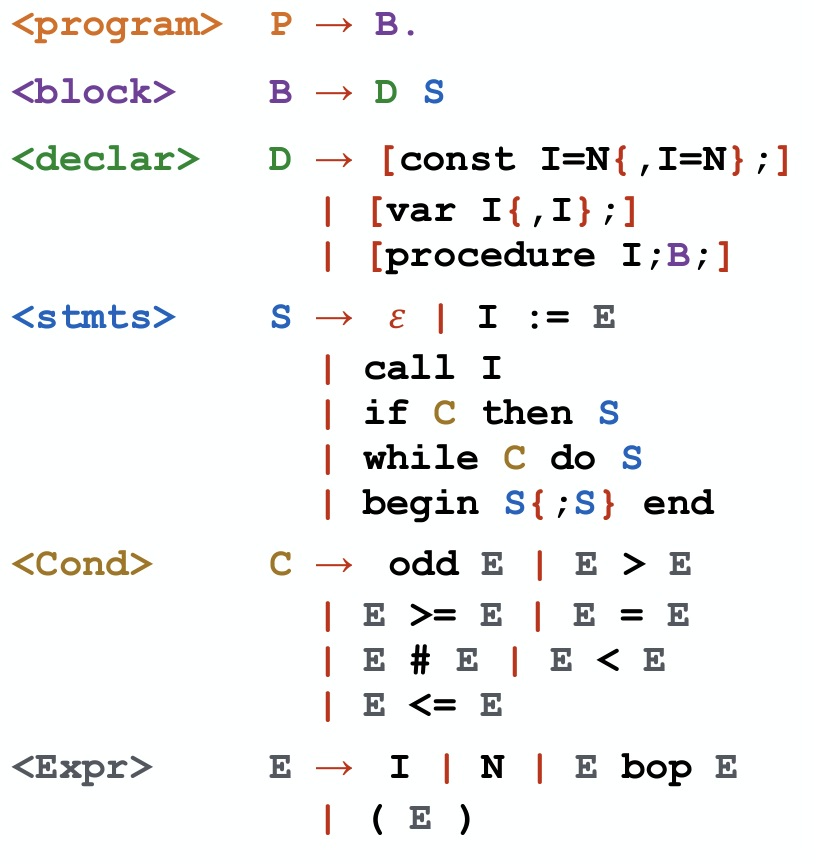
\includegraphics[width=5cm]{img/PL0.png}
  \label{fig:pl0}
\end{figure}
\begin{figure}[H]
  \centering
  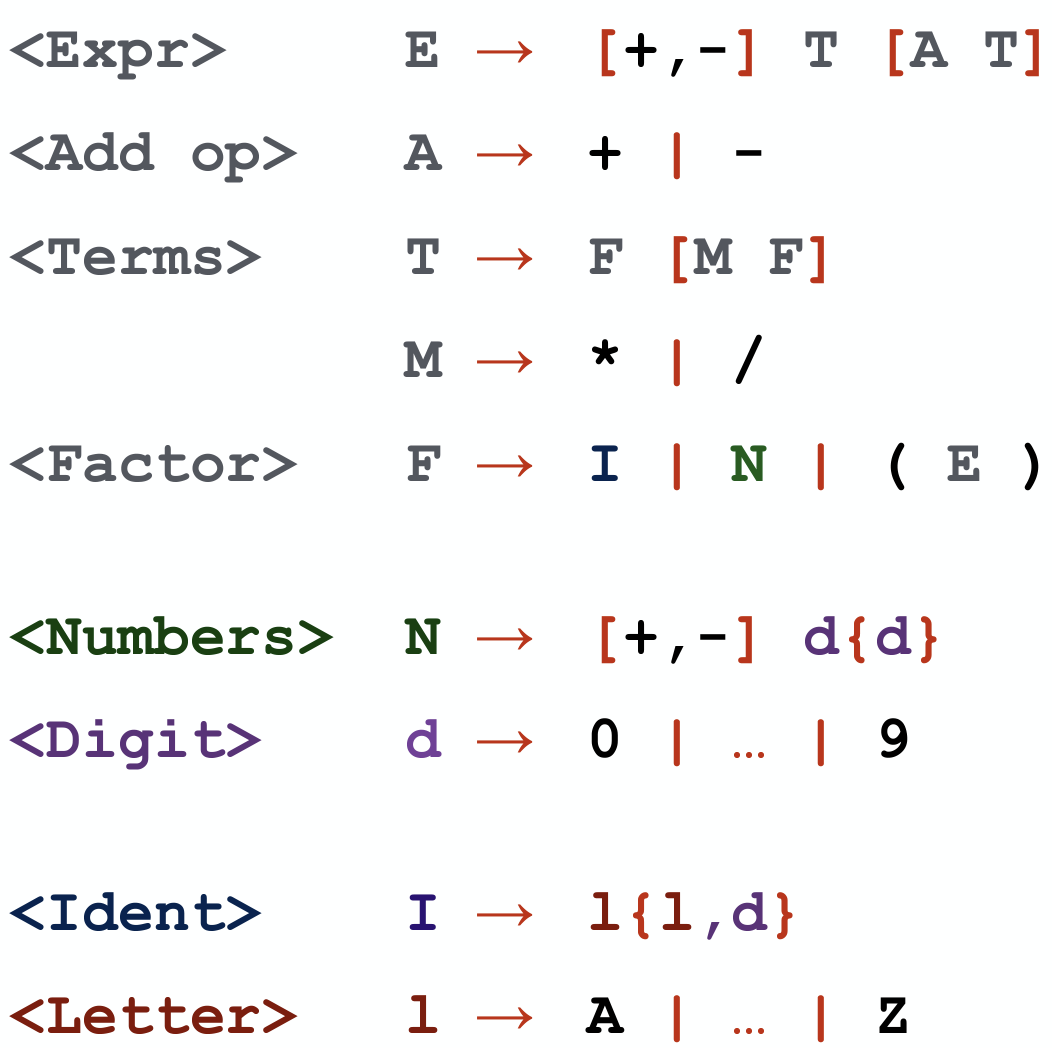
\includegraphics[width=5cm]{img/gramm_PL0.png}
  \label{fig:gramm_pl0}
\end{figure}
Permette di evitare di scrivere parentesi su tutte le espressioni
\chapter{Espressioni}
\section{Descrivere le espressioni}
\begin{tcolorbox}[title={Espressioni}]
Categoria sintattica che permette di manipolare e denotare valori.
\end{tcolorbox}
Vengono denotate per restituire il valore che rappresentano.
Due espressioni possono essere diverse sintatticamente, ma rappresentare 
un unico concetto, in questo caso saranno \textbf{equivalenti}.
\begin{itemize}
  \item $x + 1$ e $2x - x + 1$ sono uguali per ogni valore di $x$.
  \item $2x$ e $x + 2$ potrebbero essere uguali prendendo come riferimento 
  la memoria.
\end{itemize}
\begin{tcolorbox}[title={Valori esprimibili}]
Sono valori denotabili mediante una espressione, ovvero
che possono essere restituiti dalla valutazione di una espressione.
\end{tcolorbox}
Quindi sono quelli che nel nostro linguaggio saranno rappresentabili mediante espressioni,
per noi \verb|Eval = Bool| $\cup$ \verb|int|.

Gli elementi base che servono per definire le espressioni sono valori, operatori e 
gli identificatori.

\subsection{Come si caratterizzano}
Entriamo ora nel merito di come possono essere fatte le espressioni
e di quali aspetti le caratterizzano.  Abbiamo già visto che possiamo
descrivere la grammatica delle espressioni in modo che questi aspetti
siano almeno in parte risolti dalle regole grammaticali, anche se per
dare poi semantica useremo una grammatica potenzialmente più semplice.
Vediamo nel dettaglio le caratteristiche  più importanti: 
\begin{itemize}
  \item Arietà degli operatori: a quanti operandi si applica l'operatore.
  \item Notazione dell'operatore: notazione prefissa, postfissa, prefissa.
  \item Regola di precedenza: stabilisce una gerarchia sugli operatori.
  \item Regole di associatività: cosa verrà eseguito in precedenza a parità di precedenza.
  \item Ordine di valutazione.
  \item Presenza di Side-Effects: espressioni che agiscono su altre modifiche
  (\textit{ad esempio modifiche di memoria}).
  \item Overloading degli operatori: a seconda del tipo di operandi hanno effetti 
  diversi.
  \item Espressioni con tipi misti.
\end{itemize}
Ogni linguaggio potrebbe portare effetti più sottili rispetto ad altri linguaggi.
\section{Notazione}
Le espressioni aritmetiche sono una rappresentazione familiare,
fortemente basata su strumenti matematici elementari, ma anche in casi semplici
facciamo assunzioni su vari aspetti che la caratterizzano
(\textit{ad esempio sulle precedenze degli operatori}). Tali
assunzioni possono dipendere da vari aspetti e tolgono ambiguità
alla grammatica specificando un aspetto del controllo relativo alla
valutazione delle espressioni. A seconda di come si rappresenta
l’espressione varia il modo con cui si determina la semantica e di
conseguenza può variare la sua valutazione Le espressioni possono
essere denotate in modi diversi: 
\begin{itemize}
  \item Notazione infissa: ha senso sugli operatori binari, $a + b$.
  \item Notazione postfissa: utilizzata nei linguaggi funzionali $ a \, b\,+$.
  \item Notazione prefissa: notazione polacca $+\, a \, b$.
\end{itemize}
La scelta della notazione può determinare le regole di associatività e/o
precedenza, o incidere su altre caratteristiche delle espressioni. 

La più usata nelle espressioni aritmetiche è quella infissa perché di più
facile ed intuitiva lettura, però è quella in cui ho bisogno di
specificare altre regole (\textit{associatività e precedenza}) o strumenti
(\textit{le parentesi}) per eliminare ambiguità. Infatti, nelle 
altre notazioni, l’arietà dell’operatore (\textit{ovvero il numero di operandi
a cui si applica}) è spesso sufficiente ad evitare ambiguità nella
valutazione.
\subsection{Notazione post-fissa}
In questa notazione non servono regole di precedenza, regole di associatività e 
parentesi.
Necessita di uno stack e input = sequenza di simboli (\textit{operatori e operandi}).
\subsubsection{Algoritmo di valutazione}
\begin{enumerate}
  \item Leggi il prossimo simbolo di input;
  \item Se operatore:
  \begin{enumerate}
    \item applica l'operatore agli elementi in cima allo stack (\textit{in 
    funzione dell'arietà dell'operatore}).
    \item eliminiamo gli elementi usati dallo stack;
    \item salviamo il risultato in cima allo stack.
  \end{enumerate}
  \item Se operando: salvo il valore in cima allo stack;
  \item Se la sequenza non è vuota torna a $(1)$.
\end{enumerate}
\subsection{Notazione pre-fissa}
In questa notazione non servono regole di precedenza, regole di associatività e 
parentesi.
Necessita di uno stack e input = sequenza di simboli (\textit{operatori e operandi}).
\subsubsection{Algoritmo di valutazione}
\begin{enumerate}
  \item Leggi il prossimo simbolo di input;
  \item Se operatore:
  \begin{enumerate}
    \item $C_{op} = n$ (\textit{arietà dell'operatore}).
    \item  Torna a $(1)$.
  \end{enumerate}
  \item Se operando:
  \begin{itemize}
    \item se $C_{op} --$ (\textit{decremento $C_{op}$}).
    \item se $C_{op} = 0$:
    \begin{itemize}
      \item  Estraggo dallo stack gl ultimi operandi e l'operatore 
      successivo.
      \item Calcolo il valore dell'operatore applicando gli operandi 
      \item Salvo il risultato sullo stack;
      \item Decremento $C_{op}$ del successivo operatore sullo stack.
      \item Torna ad (3).
    \end{itemize}
  \end{itemize}
  \item Se la sequenza non è vuota torna a $(1)$.
\end{enumerate}
\subsection{Notazione infissa}
La notazione infissa ha bisogno di regole di precedenza, regole di associatività 
e parentesi.
Per ordine di precedenza abbiamo:
\begin{enumerate}
  \item Parentesi;
  \item Operatori unari;
  \item $**$
  \item $*\, , \, /$
  \item $+\,-$
\end{enumerate}
Per ordine di associatività intendiamo in quale ordine applicare operatori che sono 
allo stesso livello di precedenza.
La classica regola di associatività è da sinistra verso destra.
\subsection{Ordine di valutazione degli operandi}
L’implementazione di un linguaggio di programmazione deve ovviamente
rappresentare internamente le espressioni in modo da poterle manipolare.
Tipicamente la rappresentazione interna delle espressioni consiste in
una rappresentazione ad albero (\textit{abstract syntax tree}), dove i nodi
interni sono operatori mentre le foglie sono valori (\textit{ovvero operandi elementari}).
Ogni nodo interno, etichettato con un operatore, ha per figli gli
alberi che rappresentano le espressioni a cui l’operatore si applica.
L’albero fornisce q ui ndi la str utt ura dell’espressione, ovvero
elimina eventuali ambiguità legati a precedenze e associatività,
ma non può d are informazioni riguardanti l’ordine di valutazione
dell’espressione che invece è determinata dalla tipologia di visita
che l’implementazione del linguaggio effettua sull'albero. Va
notato che il problema dell’ordine di valutazione non è un problema
matematico, in quanto le operazioni sono tutte commutative, ma è un
problema informatico, in quanto ci sono vari aspetti (\textit{non propriamente
matematici}) che possono influire sul risultato: 
\begin{itemize}
  \item Operandi non definiti: La presenza di operandi non definiti può far si
  che l’espressione risultante possa essere valutata solo con un preciso
  ordine di valutazione. Si consideri, ad esempio, l’espressione di
  C \verb|(a == 0 ? b : b/a)|, è chiaro che \verb|b/a| può essere una
  divisione per 0, quindi non definita. È anche vero che, per come
  è scritta l’espressione, serve valutare \verb|b/a| solo quando a non è 0.
  Quindi in realtà, valutando le operandi solo quando necessario
  (\textit{valutazione lazy}) questa espressione è sempre definita.
  È chiaro quindi che è importante sapere se un linguaggio usa
  valutazione lazy o eager (\textit{ovvero se tutti gli operandi vengono
  comunque valutati}) per poterlo usare correttamente.
  Nel caso di espressioni booleane, la valutazione lazy è spesso
  detta corto circuito. Altri esempi sono:
  \[
    a == 0\quad || \quad b/a > 2
  \]
  Dove \verb|b/a| potrebbe essere valutato con a uguale a $0$
  \begin{lstlisting}
p := lista;
while (p != nil ) and (p.valore != 3)
  do p := p.prossimo;
  \end{lstlisting}
  Dove \verb|p.valore| potrebbe essere usato con \verb|p| uguale a \verb|nil|. 
  \item Effetti collaterali: Sono effetti non propriamente legati
  all’oggetto che si sta manipolando (\textit{ad esempio se la valutazione
  di una espressione causa anche un cambiamento della memoria}). Si
  parla di side effect anche quando una funzione modifica i propri
  parametri o comunque modifica variabili non locali. Ad esempio,
  \verb|((a+f(b)) * (c+f(b)))| con \verb|f(b)| definita come \verb|b++|,
  restituisce valori diversi a seconda dell’ordine di valutazione.
  Per evitare tali, problemi alcuni linguaggi (\textit{Java}) fissano l’ordine
  di valutazione, altri non permettono la definizione di funzioni
  con effetti collaterali. 
  \item Aritmetica finita: Nelle macchine l’aritmetica è limitata
  dall'architettura, quindi i numeri non sono infiniti ed esiste
  un massimo numero rappresentabile. Il problema di valutazione si
  ha in caso di espressioni che coinvolgono tale massimo numero, ad
  esempio se eseguiamo una somma prima di una differenza può cambiare
  il risultato se la somma calcola un numero maggiore del massimo
  numero rappresentabile. Nei linguaggi di programmazione, tipicamente
  l’ordine di valutazione risolve per prima cosa le variabili, e le
  costanti poi valuta gli operandi seguendo la struttura data dalle
  parentesi dell’espressione.
\end{itemize}
\section{Semantica}
Il significato di una espressione è essenzialmente un valore potenzialmente con 
dei vincoli (\textit{ad esempio il tipo}) ma comunque un valore. 

Le espressioni devono essere valutate per restituire un valore. I valori 
sono parte dello specifico linguaggio di programmazione. 

Due espressioni possono essere diverse, ma essere valutate nello stesso valore: in 
tal casi sono dette equivalenti. Perché due espressioni siano equivalenti non basta 
che denotino lo stesso valore in stati specifici, ma lo devono denotare in tutti gli 
stati possibili.
\subsection{Semantica nelle espressioni}
Introduciamo ora la semantica delle espressioni di un linguaggio 
imperativo (\textit{basato su architettura di von Neumann}), che chiamiamo 
\verb|IMP|. Per parlare della semantica non ci interessa la grammatica 
che include tutte le regole di associatività e di precedenza, ma 
ci basta quella più semplice anche se ambigua. Di fatto nella semantica
si rappresenta, mediante la forma sintattica, il corrispondente albero
di valutazione che è invece non ambiguo. Ignoriamo anche le parentesi
per semplificare, visto che le regole, essendo induttive, non ne sono
influenzate (\textit{il caso $\mathcal{E}$ sarebbe un caso induttivo che toglierebbe 
solo le parentesi, quindi chiaramente senza rilevanza semantica}).
Quindi per parlare di semantica guardiamo alla struttura induttiva e 
non alla struttura sintattica (\textit{ignoriamo gli aspetti puramente lessicali}). 
Ad esempio con l’espressione $\mathcal{E} + \mathcal{E}$ stiamo rappresentando un albero
sintattico con come radice $+$ ed i cui sottoalberi (\textit{operandi}) sono 
espressioni, quindi generati a loro volta da $\mathcal{E}$

Ricordiamo che la sintassi che abbiamo introdotto per le espressioni è la seguente:
\[
\begin{matrix}
  \mathcal{E} & \longrightarrow & \mathcal{A}& | &\mathcal{B} & & & & & \\
  \mathcal{A} & \longrightarrow & \mathcal{I} &| & \mathcal{N} &
  | & \mathcal{A} \,op\,\mathcal{A} & & & \\
  \mathcal{B} & \longrightarrow & \mathcal{I} &| & true & | & false & | &
  not\,\mathcal{B} & \\
  & & & | & \mathcal{B} \,or\,\mathcal{B} & | & \mathcal{A} \,=\,\mathcal{A}
\end{matrix}
\]
Dove $\mathcal{A}$ sono le espressioni aritmetiche in cui \verb|op| sta nell'insieme 
\{$+,-,*,=$\}, mentre $\mathcal{B}$ sono le espressioni booleane.

VIsto che gli identificatori hanno un significato che coinvolge anche i comandi 
oltre che i concetti di ambiente e binding, cerchiamo di capire prima le espressioni 
ignorando gli identificatori, ovvero assumiamo espressioni senza identificatori.
Ovvero partiamo a dare significato alla seguente grammatica delle espressioni:
\[
\begin{matrix}
<EXP> & \mathcal{E} & \longrightarrow & \mathcal{A} & | & \mathcal{B}\\
      & \mathcal{A} & \longrightarrow & \mathcal{N} & | & \mathcal{A}\,op\,\mathcal{A}\\
      & \mathcal{B} & \longrightarrow & | & true & | & false \\
      & & &| & not \, \mathcal{B} & | &
      \mathcal{B} \,or\,\mathcal{B} & | & \mathcal{A} \,=\,\mathcal{A}
\end{matrix}
\]
Per prima cosa dobbiamo definire l'insieme $\mathcal{E}$ delle espressioni da valutare 
ad intero o booleano, ovvero quelli che prima abbiamo detto essere alberi di valutazione, 
con metavariabile $e$.
\begin{tcolorbox}[title = {Espressioni $\mathcal{E}$}]
  Insieme di (\textit{alberi di valutazione}) di espressioni valutate ad intero o booleano: $e$.
\end{tcolorbox}
Dobbiamo anche definire l'insieme dei valori, ovvero dei numeri della macchina
sottostante, e dei valori booleani. È da notare che la macchina sottostante non 
è necessariamente una macchina fisica, può infatti essere una macchina virtuale.
\begin{tcolorbox}[title = {Numeri $\mathcal{N}$}]
  Insieme di numerali nella macchina sottostante: $m,n,p$.
\end{tcolorbox}
\begin{tcolorbox}[title = {Booleani $\mathcal{B}$}]
  Insieme di valori booleani \{\verb|true|, \verb|false|\}: $t$.
\end{tcolorbox}
Infine usiamo questi insiemi per definire il sistema di transizione, le cui regole 
forniranno esattamente la semantica operazionale delle espressioni di cui abbiamo dato 
la grammatica.

Quindi definiamo l'insieme delle configurazioni $\Gamma$ co e l'insieme delle espressioni 
da valutare $\mathcal{E}$. L'insieme delle configurazioni terminali $\mathcal{T}$
sono ovviamente i valori. Come sappiamo, le configurazioni terminali devono essere un 
sottoinsieme delle configurazioni, ed effettivamente i valori sono espressioni primitive.
A partire da questi insiemi possiamo definire il sistema di transizione:
\begin{tcolorbox}[title ={Sistema di transizione}]
  \[
  \begin{matrix}
  \Gamma = \mathcal{E} & \mathcal{T} = \mathcal{N}\,\cup\,\mathcal{B} &
  op \in \{+,-,*,=\} &bop\in \{=,or\}  
  \end{matrix}
  \]
\end{tcolorbox}
\section{Regole di transizione}
A questo punto introduciamo le regole di transizione.
\begin{itemize}
  \item La prima regola è un assioma, che semplicemente valuta l'espressione sintattica 
  contenente un operatore aritmetico, nel valore che esso rappresenta. Ad esempio la semplice operazione $3+5 = 8$
  \[
    \begin{matrix}
      \mathcal{E}_1: & m \quad op\quad n &\rightarrow &p
    \end{matrix}
  \]
  \item La seconda regola è invece una regola induttiva di valutazione. questa 
  regola mi dice che, se gli operandi non 
  sono valori primitivi allora dobbiamo valutarli. In particolare, questa regola 
  mi dice che prima valutiamo l'espressione a sinistra dell'operatore. 
  \[
  \infer[\scriptscriptstyle (\mathcal{E}_2)]
  {
    e \quad op \quad e_0 \longrightarrow e' \quad op \quad e_0
  }
  {
    e \longrightarrow e'
  }
  \]
\item La terza regola stabilisce che nel momento in cui l'operando a sinistra è un valore allora 
posso iniziare a valutare l'operando a destra.

Chiaro che quando anche l'operatore a destra è un valore allora 
ricadiamo nell'assioma e possiamo restituire il valore finale.
\[
  \infer[\scriptscriptstyle (\mathcal{E}_3)]
  {
    m \quad op \quad e \longrightarrow m \quad op \quad e'
  }
  {
    e \longrightarrow e'
  }
  \]
  \item Per permettere la derivazione dobbiamo aggiungere una nuova regola, ma questa 
  rende il sistema di transazione non deterministico perché quando abbiamo 
  un operatore applicato a due espressioni non costanti, abbiamo almeno due regole che possiamo 
  applicare e quindi due transazioni possibili.
  Ci possono essere problemi quando, nel linguaggio, il valore 
  risultato può dipendere dall'ordine di valutazione degli operandi, e questo 
  non va bene, per questo nella semantica si tende a dare un ordine fissato.
  Quindi le regole $\mathcal{E}_1, \mathcal{E}_2$ permettono solo la valutazione da sinistra verso destra.
  Mentre $\mathcal{E}_6$ permetterebbe una valutazione indipendente dei due
  sottoalberi, più coerente con i possibili modi di valutare un’espressione,
  ma con maggiore possibilità di errore nell’implementazione.
  Quindi potremmo dare più regole ma non è necessario e può essere
  controproducente, anche se così perdiamo alcune proprietà matematiche,
  come la commutatività.
  \[
    \infer[\scriptscriptstyle (\mathcal{E}_6)]
  {
    e_0 \quad op \quad e \longrightarrow e_0 \quad op \quad e'
  }
  {
    e \longrightarrow e'
  }
  \]
Osserviamo quindi come nella semantica tutto quello che
specifichiamo è possibile, mentre quello che non si può derivare
da quanto specificato non è possibile, viceversa tutto quello che
è derivabile dalle regole deve essere desiderato (\textit{altrimenti abbiamo
sbagliato la specifica}). Non è invece possibile specificare cosa non
vogliamo derivare.
\item Questa regola è un assioma, che semplicemente valuta l'espressione sintattica 
contenente un operatore, nel valore che esso rappresenta, chiaro che se
l’operatore è booleano i valori coinvolti devono essere entrambi
booleani (\textit{di questa verifica si parlerà più avanti}).
\[
  \begin{matrix}
    \mathcal{E}_4: \qquad k_1 \quad bop\quad k_2\rightarrow t \\
    k_1,k_2 \in \mathcal{B}\cup \mathcal{N} \quad t \in \mathcal{B} \quad bop \in \{=,or\}
  \end{matrix}
\]
\item La regola successiva è esattamente la regola $\mathcal{E}_3$ dove ammettiamo
che l’espressione contenga operatori binari booleani. Anche in questo
caso fissiamo l’ordine di valutazione da sinistra verso destra.
\[
  \infer[\scriptscriptstyle (\mathcal{E}_2)]
  {
    e \quad bop \quad e_0 \longrightarrow e' \quad bop \quad e_0
  }
  {
    e \longrightarrow e'
  }
  \]
  \item La regola successiva stabilisce invece che, nel momento in
  cui l’operando a sinistra è un valore booleano allora posso iniziare
  a valutare l’operando a destra. Chiaro che, nuovamente, quando anche
  l’operatore a destra è un valore booleano allora ricadiamo
  nell’assioma $\mathcal{E}_4$ e possiamo restituire il valore finale.
  \[
  \infer[\scriptscriptstyle (\mathcal{E}_5)]
  {
    t \quad bop \quad e \longrightarrow t \quad op \quad e'
  }
  {
    e \longrightarrow e'
  }
  \]
  \item Nel caso booleano, dobbiamo aggiungere la regola per
  l’operatore unario. Per prima cosa l’assioma che restituisce 
  il valore corrispondente all’applicazione dell’operatore sul
  valore rappresentato, e poi la regola di valutazione, analoga
  alle precedenti.
  \[
    \begin{matrix}
      \mathcal{E}_6: &not \quad t_1 & \longrightarrow & t
    \end{matrix}
  \]
  \[
    \infer[\scriptscriptstyle (\mathcal{E}_7)]
    {
      not \quad e \longrightarrow not \quad e'
    }
    {
      e \longrightarrow e'
    }
    \]
\end{itemize}
\subsection{Valutazione di equivalenza}
Come abbiamo più volte sottolineato, le regole della semantica dinamica, ovvero 
del sistema di transizione, descrivono formalmente come vengono valutate le 
espressioni del nostro linguaggio. Quindi, possiamo usare queste regole per definire 
formalmente cosa significa valutare un'espressione.

Sia $k$ una costante (\textit{intero o booleano}). Formalmente $k$ è il significato 
di un oggetto (\textit{simbolo}) sintattico $k$ dentro $\mathcal{N}\cup\mathcal{B}$.
Nel nostro caso quindi $k$ è un valore dentro $\mathbb{N}\cup\mathbb{B}$, ovvero numeri 
interi e booleani. Allora la valutazione è una funzione che prende una espressione 
in $\mathcal{E}$ (\textit{configurazione del sistema di transizione}) e gli associa 
il valore che esso rappresenta.
\begin{tcolorbox}[title ={Valutare delle espressioni}]
  La valutazione è una funzione \verb|Eval|: $\mathcal{E} \rightarrow \mathbb{N}\cup\mathbb{B}$
  che descrive il comportamento dinamico delle espressioni restituendo il valore in cui esse 
  sono valutate:
  \[
    \verb|Eval|(e)=k \Longrightarrow e \rightarrow^* k
  \]
\end{tcolorbox}
dove $\rightarrow^*$ è la chiusura transitiva della relazione di transizione $\rightarrow$.

A questo punto, il concetto di valutazione può essere usato per definire formalmente quando due espressioni 
sono equivalenti, ovvero quando due espressioni anche diverse sintatticamente, 
rappresentano invece lo stesso valore, ovvero hanno lo stesso significato.
\begin{tcolorbox}[title = {Equivalenza di espressioni}]
  L'equivalenza di espressioni è una relazione $\equiv \subseteq \mathcal{E} \times \mathcal{E}$
  definita come segue:
  \[
    e_0 \equiv e_1 \Longrightarrow \verb|Eval|(e_0)\equiv\verb|Eval|(e_1)
  \]
\end{tcolorbox}
Grazie a questa definizione, possiamo quindi dimostrare che, ad esempio, l'espressione $(3+5)\cdot 2$ è 
equivalente a $(1+3)\cdot 4$, pur essendo due espressioni sintatticamente molto diverse.

\chapter{Dichiarazioni}
\section{Identificatori}
\begin{tcolorbox}[title = {Identificatori}]
  Sequenza di caratteri usata per rappresentare o denotare un altro oggetto.
\end{tcolorbox}
Gli identificatori sono sequenze di caratteri, che hanno lo scopo 
di denotare qualcos'altro. Gli identificatori sono quindi dei nomi (\textit{definiti 
da regole specifiche per ogni linguaggio}) usati per riferire altri elementi del linguaggio
(\textit{es. procedure}) 
o della macchina sottostante (\textit{celle di memoria}) durante la computazione, 
senza necessariamente conoscerne il valore a priori. Quando identificano celle di memoria, 
gli identificatori sono anche detti variabili, anche se il concetto di variabile è 
qualcosa di più complesso come vederemo.

L'uso di nomi è fondamentale perché oggetti simbolici sono più facili da ricordare, e 
perché permettono di attuare un processo di astrazione, sia sui dati che sul controllo.
Deve essere chiaro che identificatore e oggetto denotato non sono la stessa cosa: un 
identificatore può denotare più elementi, un elemento può 
essere denotato da più identificatori (\textit{aliasing}).
\begin{algorithm}
  const pi = 3.14;  //costante
  int x;            //variabile
  void f(){...}     //procedura
\end{algorithm}
Per ciò che riguarda il processo di astrazione, l'uso degli identificatori 
ci permette di sostituire gli indirizzi assoluti della memoria con dei nomi, 
rendendo i programmi più facili da leggere e risolvendo anche il problema 
dell'indirizzamento assoluto, in quanto il programmatore 
non deve necessariamente sapere dove e come un valore viene memorizzato 
per poterlo usare.

Gli identificatori non possono essere stringhe di caratteri qualunque, ma devono 
seguire delle regole in modo che il parser del linguaggio li possa 
riconoscere come tali, per non confonderli per parole chiave del linguaggio stesso.

Quindi ogni linguaggio ha le sue regole che normalmente rispondono ad una serie 
di quesiti che ci dobbiamo porre quando studiamo un linguaggio nuovo:
\begin{itemize}
  \item Gli identificatori sono o non sono case-sensitive? 
  \item Esistono parole riservate del linguaggio?
  \item Ci sono vincoli di lunghezza?
  \item Ci sono caratteri speciali per specificare identificatori?
\end{itemize} 
\section{Bindings}
Il concetto di binding viene ereditato dalla matematica. In matematica i nomi si 
usano per denotare oggetti complessi. Prima di poterli usare, dobbiamo creare 
il legame, ovvero \textbf{dichiarare} il nome e definire il suo significato.
In questo consiste quindi la creazione del legame nelle così dette occorrenze 
di binding.
\[
  \left(\sum_{i=1}^{n}\left(\sum_{j=1}^{m} a_{ij}\dots b_{jk}\right)\right)
\]
Viene definito il \textbf{nome} (\textit{identificatore}) e il suo 
\textbf{significato} (\textit{denotazione}).

In programmazione i binding sono creati dalle dichiarazioni. Successivamente 
il nome può essere correttamente usato per riferirsi/rappresentare il suo significato.
Questi usi sono chiamati occorrenze di applicazione.
\[
  \left(\sum_{i=1}^{n}\left(\sum_{j=1}^{m} a_{\textcolor{blue}{ij}}\dots b_{\textcolor{blue}{j}k}\right)\right)
\] 
Viene usato il \textbf{nome} (\textit{identificatore}) per accedere al suo 
\textbf{significato} (\textit{denotazione}).
\subsection{Binding e scope}
In generale, un nome non dichiarato, di cui non è stato descritto il significato 
è un nome che può rappresentare qualunque cosa in quel punto.
Quindi una sua occorrenza può essere legata a qualunque oggetto, e per questo viene chiamata
occorrenza libera.

Dobbiamo osservare che in realtà dal punto di vista del costrutto le occorrenze libere e quello applicate 
sono identiche, la differenza consiste nell'essere nel raggio di azione (\textit{scope}) di una occorrenza 
di definizione.
\begin{tcolorbox}[title={Scope di un binding}]
Definisce lo spazio in cui si può usare un nome per rappresentare il significato associato 
ad un binding.
\end{tcolorbox}
\subsection{Bindings nei linguaggi di programmazione}
Nei linguaggi di programmazione i concetti di bindings e scope prendono una connotazione 
propria. Quindi ci chiediamo cosa significa definire e usare identificatori nei linguaggi 
di programmazione. Partiamo da un esempio: \verb|const x=10;| \verb|var y=1;| \verb|y:=x+y|.
In questo caso, la prima occorrenza di \verb|x| e la prima di \verb|y| sono occorrenze 
di definizione perché definiscono \verb|x| e \verb|y| come nomi di 
oggetti che rappresentano valori interi.
Nel caso di \verb|x| abbiamo un nome che avrà sempre un valore costante,
nel caso di \verb|y| invece abbiamo un nome il cui valore può cambiare 
durante la computazione. Tutte le occorrenze nell'assegnamento sono invece 
applicazione in quanto l'assegnamento non definisce identificatori ma ne aggiorna 
il valore.

In generale è il PL che definisce (\textit{sintatticamente e semanticamente}) cosa è 
definizione e cosa è uso di un identificatore, inoltre ci sono PL in cui un programma 
completo (\textit{incluse librerie}) non sono ammesse occorrenze libere di identificatori.
Abbiamo già detto che i binding ci permettono di usare dei nomi per riferirsi a significati
(\textit{ovvero gli oggetti denotati)}. Ma perché fare questo
passaggio? Chiaramente, i nomi sono oggetti simbolici e gli 
oggetti simbolici sono in generale più facili da ricordare 
(\textit{un identificatore è più facile da ricordare di un indirizzo
fisico}). Ma il motivo più importante è che permettono
astrazione, ovvero ci permettono di riferirci ad un oggetto
denotato senza conoscere tutti i dettagli: ci possiamo
riferire al contenuto di una cella attraverso l’identificatore
senza sapere l’effettivo indirizzo fisico. Questo garantisce
anche la possibilità di dare significato in modo indipendente
dalla macchina su cui poi il programma viene eseguito.
\subsection{Tipi di bindings nei linguaggi di programmazione}
I binding possono legare nomi a diversi tipi di significato, 
permettendo sia astrazione sui dati che astrazione sul controllo.
A seconda dell'oggetto denotato il binding creato è di tipo diverso. Quando 
il legame non può cambiare allora si lega il nome ad un valore (\textit{sia 
il valore di una costante, il tipo della variabile, o qualunque altra informazione 
immutabile dopo la definizione}).

Quando abbiamo una variabile, questa può essere modificata durante 
il binding alla memoria, ma il valore del suo contenitore, nel senso che l'informazione 
del contenitore, legata al nome, non cambia, cambia solo il valore associato.
Questa situazione viene modellata combinando due binding: Nome-locazione (\textit{legame non modificabile}) e 
locazione-valore (\textit{legame modificabile}), il primo fissato dalla 
definizione il secondo modificabile dall'esecuzione.

Tutti i legami sono immutabili dopo la definizione sono detti statici.
\begin{tcolorbox}[title = {Binding statico}]
  Un binding è statico se occorre per la prima volta dall'esecuzione e 
  rimane invariato durante tutta l'esecuzione del programma.
\end{tcolorbox}
Sono binding statici, ad esempio, i tipi delle variabili nei linguaggi fortemente tipati.

I legami che possono cambiare durante l'esecuzione sono detti legami dinamici:
\begin{tcolorbox}[title = {Binding dinamico}]
  Un binding dinamico se occorre durante l'esecuzione è può variare.
\end{tcolorbox}
Sono binding dinamici, ad esempio, quelli tra locazioni/celle di memoria e valori 
contenuti nelle locazioni.
\subsection{Tempi di binding}
È importante anche stabilire quando avviene la creazione dei binding:

\begin{minipage}[t]{0.45\textwidth}
  \textbf{Early binding:}
  
  \begin{itemize}
      \item C
      \item Fortran
      \item COBOL
      \item Pascal (in parte)
  \end{itemize}
  
  \end{minipage}\hfill
  \begin{minipage}[t]{0.45\textwidth}
  \textbf{Late binding:}
  
  \begin{itemize}
      \item Pascal (in parte)
      \item Snobol4
      \item LISP
      \item APL
  \end{itemize}
\end{minipage}  

A sinistra, per ogni nome tutto viene risolto a tempo di
compilazione, quindi abbiamo una allocazione statica della memoria, 
con tutti gli indirizzi assoluti, questo rende l'esecuzione estremamente 
veloce ma la programmazione poco flessibile.

A destra tutto avviene a tempo di esecuzione, quindi la memoria 
viene allocata dinamicamente, tutti i binding vengono creati dinamicamente con indirizzi 
non assoluti.
Questo rende l'esecuzione più lenta, ma la programmazione puù flessibile.
Altri linguaggi stanno nel mezzo allocando solo quando serve, ad esempio in presenza 
di ricorsione come in C.
\section{Identificatori, ambienti e dichiarazioni}
Nei linguaggi di programmazione, per riferire valori generati dalle espressioni
usiamo il concetto di identificatore. Un identificatore è di
fatto un nome che viene associato all’oggetto da identificare/riferire.
Un nome è una sequenza di simboli usata per rappresentare qualcosa,
permettendo un processo di astrazione (\textit{ad esempio, locazioni e
funzioni}): abbiamo un’entità che ricorre più volte o che sarebbe
complesso descrivere all’interno di una frase, e quindi le diamo
un nome e con il suo identificatore rappresentiamo il suo significato.

Per riferire i valori (\textit{oggetti denotabili}) associati agli identificatori
usiamo il concetto di ambiente, definito come insieme di legami (\textit{bindings})
tra identificatori e oggetti denotabili, ovvero tutti quegli oggetti
del nostro linguaggio che sono riferibili mediante un identificatore.
Solitamente, quando si parla di ambiente ci si riferisce solo alle associazioni
che non sono stabilite dalla definizione del linguaggio, ma dal programmatore.
Quindi è quella componente della macchina astratta che per ogni nome
introdotto dal programmatore, e per ogni punto di programma, permette
di determinare quale sia l’associazione corretta. Va osservato che l’ambiente non esiste al livello della macchina fisica, fa parte delle caratteristiche dei linguaggi ad alto livello e quindi deve essere opportunamente simulato nelle implementazioni.

La dichiarazione implementa la creazione dei legami. In
generale, le occorrenze in una espressione (\textit{ovvero le
occorrenze di uso}), sono \textbf{free occurrences}. Se vogliamo dar loro significato dobbiamo rendere tali occorrenze
applied occurrences inserendole nello scope di binding occurrences. Quindi le dichiarazioni forniscono le binding
occurrences che, dando significato all’identificatore, prima del suo
uso, lo rendono legato e non più libero.
\begin{tcolorbox}[title = {Ambiente}]
  L'ambiente è insieme delle associazioni fra nomi e oggetti denotabili esistenti a
  run-time in uno specifico punto del programma ed in uno specifico momento
  dell’esecuzione.
\end{tcolorbox}
\begin{tcolorbox}[title = {Dichiarazione}]
  La dichiarazione è meccanismo (\textit{implicito o esplicito}) col quale si crea un’associazione nell’ambiente.
\end{tcolorbox}
\subsection{Termini chiusi e ground}
\begin{tcolorbox}[title = {Termine chiuso}]
  In un linguaggio (\textit{con identificatori}), un termine chiuso in cui non 
  ci sono identificatori liberi è detto chiuso.
\end{tcolorbox}
Il significato delle frasi chiuse è consiste nel poter dare significato alla
frase senza richiedere un ambiente esterno. In termini
di linguaggi di programmazione, significa che un programma
Pascal completo, ad esempio, non ha FI (\textit{identificatori liberi}) e
quindi può essere eseguito a partire da un ambiente vuoto, in
quanto non ci sono identificatori che richiedono un
significato all’esterno.

Ad esempio, non possiamo dare significato ad \verb|a+b+c+x| se
non viene dato un significato ad \verb|a|, \verb|b|, \verb|c| e \verb|x|.
Abbiamo bisogno
quindi di assunzioni sull'ambiente, che consiste sull'insieme
di binding per gli identificatori, e i binding non sono
altro che uguaglianze del tipo \verb|nome=entità|. Quindi un
programma è una frase chiusa se ogni occorrenza d’uso è
preceduta da una occorrenza di definizione che stabilisce
il significato dell’identificatore.
\begin{tcolorbox}[title = {Termine gound}]
  In un linguaggio (\textit{con identificatori}), un termine in cui non ci sono 
  identificatori è detto ground.
\end{tcolorbox}
Chiaramente un termine ground non richiede nemmeno
un ambiente non avendo identificatori. La prima versione
della categoria sintattica delle espressioni che abbiamo
dato è costituita solo da termini ground (\textit{non avendo inserito il termine
degli identificatore come terminale della sua grammatica}), ed
effettivamente abbiamo potuto dare
semantica alle espressioni senza parlare di ambienti.
\section{Ambienti (in IMP)}
Nel nostro semplice linguaggio imperativo consideriamo solo interi 
e booleani, quindi per il momento questi, nel nostro linguaggio sono 
gli unici oggetti denotabili:
\[
  \mathcal{N} = \text{Insieme di numerali nella macchina sottostante: }m,n,p
\]
\[
  \mathcal{B} = \{\verb|true,false|\}:\,t
\]
I valori denotabili, nel nostro linguaggio, costituiscono l'insieme 
\verb|DVal|, che quindi per ora è $\verb|Int| \cup \verb|Bool|$, ma che poi verrà 
adeguato ai vari costrutti con cui arricchiremo il linguaggio.

Possiamo ora definire formalmente il concetto di ambiente che
associa identificatori agli oggetti denotabili ($\bot$ \textit{va associato all'identificatore non definito, 
ovvero non associato ad alcun valore}). Quindi un ambiente per un 
insieme di identificatori finito $V\,(Env_V)$ è una funzione che ad ogni 
identificatore associa un valore denotabile, oppure il valore 
non definito $\bot$. L'ambiente è l'unione (\textit{disgiunta}) 
di tutte queste funzioni al variare dell'insieme $V$. Questo ambiente è detto dinamico, per 
distinguerlo poi da quello che verrà chiamato statico.
\begin{definizione}[Ambiente]
  Un ambiente dinamico è un elemento dinamico dello spazio di funzioni
  \[
    Env = \cup_{V \subseteq Id}\,Env_V
  \]
  dove $Env_V: V \rightarrow DVal\qquad \cup\{\bot\}$ ha metavariabili $\rho$
\end{definizione}
\section{Espressioni con identificatori}
Riprendiamo ora le espressioni per arricchire la loro semantica con gli 
identificatori. Quindi la sintassi ora è la grammatica completa delle espressioni:
\[
\begin{matrix}
<EXP> \\
       \mathcal{E} & \longrightarrow & \mathcal{A} & | & \mathcal{B}\\
       \mathcal{A} & \longrightarrow & \mathcal{I} & | & \mathcal{N} & | & \mathcal{A}\,op\,\mathcal{A}\\
       \mathcal{B} & \longrightarrow & \mathcal{I} & | & true & | & false \\
       & & &| & not \, \mathcal{B} & | &
      \mathcal{B} \,or\,\mathcal{B} & | & \mathcal{A} \,=\,\mathcal{A}
\end{matrix}
\]
per prima cosa dobbiamo definire $\mathcal{E}^V$ delle espressioni (\textit{con identificatori}) valutate 
ad intero o booleano, ovvero quelli abbiamo detto essere alberi di valutazione, con 
metavariabile $e$. Queste costituiscono l'insieme delle nuove configurazioni del sistema ùdi transizione. Invece, 
l'insieme dei valori (\textit{ovvero delle configurazioni terminali del 
sistema di transizione}) e valori rimangono inalterati, in quanto non cambiano con 
l'uso degli identificatori.
\begin{tcolorbox}[title = {Sistema di transizione}]
  \[
    \Gamma = \mathcal{E}^V, \mathcal{T}= \mathcal{N}\cup\mathcal{B}, op\in\{+,-,*,=\}\,bop\in \{=,or\}
  \]
\end{tcolorbox} 
Per prima cosa tutte le regole precedentemente definite per le espressioni
devono essere riscritte integrando l’ambiente nella regola, in quanto
le espressioni con identificatori devono essere valutate dentro un
ambiente. Quindi, tutte le regole $\mathcal{E}_i$ viste diventano:
\[
  \mathcal{E}_i: \rho \vdash e \rightarrow_e e'
\]
dove $\rho$ è l’ambiente di valutazione delle espressioni,
ovvero la specifica dell’associazione tra identificatori e oggetti
denotati. Infine, il pedice della freccia ($\rightarrow_e$) denota quale
sistema di transizione si sta usando (\textit{perché ne definiremo uno per
ogni categoria sintattica}).
Quindi le regole che scriviamo adesso sovrascrivono completamente
quelle già viste, per quanto facciano tutte la stessa cosa,
semplicemente dentro un ambiente $\rho$.
\subsection{Identificatori liberi}
\begin{tcolorbox}[title={Occorrenza libera}]
  Un identificatore è in posizione libera se il suo uso non è nel raggio
  d'azione di una definizione.
\end{tcolorbox}
Data una espressione o una frase scritta in un certo linguaggio, gli identificatori 
liberi sono quelli che non hanno nessuna dichiarazione che li coinvolge. Questo
significa che la frase in questione è necessariamente parte di una frase più
grande dove gli identificatori liberi sono
legati e trovano significato.
Quindi sono identificatori liberi in una espressione tutti quelli
che hanno solo occorrenze libere e non di applicazione, ovvero
occorrenze che non sono nel raggio di azione di una occorrenza di binding
(\textit{di definizione}). Dentro un'espressione, la presenza di un
identificatore libero richiede l’accesso ad un “ambiente" esterno che
gli dia significato. Quindi, ad una espressione con identificatori liberi
non possiamo dare significato.
Possiamo capire il concetto di libertà guardando alla struttura
dell’abstract syntax tree e in funzione di questo possiamo definire
gli identificatori liberi per induzione sulla struttura sintattica.
Quindi definiamo l'insieme degli identificatori che hanno occorrenze
libere all'interno di un'espressione $IMP: (bop \in \{or,=,+,-,*\},\,uop=not)$
\begin{definizione}[Identificatori liberi]
  La funzione $FI:Exp\rightarrow Id$, che ad ogni espressione associa l'insieme 
  degli identificatori liberi in essa contenuti, è definita per induzione da:
  \[
  \begin{matrix}
    FI(h)=\varnothing \\
    FI(id)=\{id\}\\
    FI(e_0 \,\verb|bop| \,e_1) = FI(e_0) \cup FI(e_1) \\
    Fi(\verb|uop| \,e)=FI(e)
  \end{matrix}  
  \]
\end{definizione}
Ovviamente così come possiamo definire gli identificatori liberi, possiamo definire anche 
quelli legati (\verb|DI|). In generale anche questi vanno definiti per induzione sulla 
struttura sintattica delle espressioni, o di una categoria sintattica. Ovviamente nel nostro
caso la definizione è molto semplice in quanto nelle espressioni non abbiamo costrutti che creano 
legami, occorrenze, ma solo costrutti che utilizzano occorrenze. Quindi l'insieme delle occorrenze 
legate/definite è vuoto. Si noti che $\verb|FI|(e)\,\cup\,\verb|DI|(e)=\verb|id|(e)$. Questo concetto 
esiste in tutti i PL.
\subsection{Regole}
Ora riportiamo le regole aggiornate con l'ambiente, quelle già descritte non 
verranno ulteriormente commentate, essendo esattamente le stessa già descritte per le 
espressioni.
\[
  \mathcal{E}_1: \rho \vdash m\,\verb|op|\,k\rightarrow_e p \qquad \text{se }m\,\verb|op|\,n = k,m,n \in \mathcal{N}\quad k \in \mathcal{N}\cup\mathcal{B}
\]
La seconda regola adesso cambia, in quanto ora ci serve l'assioma per gli identificatori:
\[
  \mathcal{E}_2 \rho \vdash I \rightarrow_e n\qquad se \qquad\rho(I)= n
\]
In questo assioma quindi diciamo che quando incontriamo un identificatore,
questo viene valutato nel valore che l’ambiente associa all’identificatore.
È chiaro che questa regola è applicabile solo se $I$ è un identificatore per
il quale in $\rho$ esiste una associazione.
\[
    \infer[\scriptscriptstyle (\mathcal{E}_3)]
    {
      \rho \vdash e \, op \, e_0 \rightarrow_e e' \, op \, e_0
    }
    {
      \rho \vdash e \rightarrow_e e'
    }
\]
\[
    \infer[\scriptscriptstyle (\mathcal{E}_4)]
    {
      \rho \vdash m \, op \, e \rightarrow_e m \, op \, e'
    }
    {
      \rho \vdash e \rightarrow_e e'
    }
\]
\[
  \mathcal{E}_5: \rho \vdash m\,\verb|bop|\,k\rightarrow_e p \qquad \text{se }m\,\verb|op|\,n = k,m,n \in \mathcal{N}\quad k \in \mathcal{N}\cup\mathcal{B}
\]
\[
    \infer[\scriptscriptstyle (\mathcal{E}_{3'})]
    {
      \rho \vdash e \, bop \, e_0 \rightarrow_e e' \, bop \, e_0
    }
    {
      \rho \vdash e \rightarrow_e e'
    }
\]
\[
    \infer[\scriptscriptstyle (\mathcal{E}_{6})]
    {
      \rho \vdash k \, bop \, e_0 \rightarrow_e k \, bop \, e'
    }
    {
      \rho \vdash e \rightarrow_e e'
    }
\]
\[
  \mathcal{E}_7: \rho \vdash \verb|not| \,t_1\rightarrow_e t \qquad \text{se }\verb|not|\,t_1 = t, \qquad t_1\in \mathcal{B}
\]
\[
    \infer[\scriptscriptstyle (\mathcal{E}_{8})]
    {
      \rho \vdash not \, e \rightarrow_e not \, e'
    }
    {
      \rho \vdash e \rightarrow_e e'
    }
\]
\section{Tipo}
Ora aggiungiamo un nuovo ingrediente al nostro linguaggio: i tipi. Il tipo determina l'insieme 
di valori (\textit{che condividono una certa proprietà strutturale}) dotato di un insieme 
di operazioni definite per i valori di quel tipo. In altre parole, il tipo determina il range di valori che
un identificatore può memorizzare/denotare e l'insieme di operazioni definite su quei valori.
A volte determina qualche informazione in più, ad esempio per i floating point il tipo determina anche al precisione.+

Esempi di tipo sono: $Integer, String, Int \rightarrow Bool, (Int \rightarrow Int) \rightarrow Bool$.
In questo caso, ogni tipo è effettivamente un insieme omogeneo di valori e di operazioni su quei valori.

Esempi di elementi che non sono un tipo: ${3, true, x \rightarrow x}$.

In questo caso, o l'elemento non è un insieme omogeneo, oppure è omogeneo, ma parziale, quindi 
non raccoglie tutti gli oggetti su cui posso operare allo stesso modo. 
Anche se non sempre questa distinzione è così netta, e dipende dal linguaggio. I 
tipi sono utili a vari livelli per molti diversi:
\begin{itemize}
  \item Livello di progetto: organizzano l'informazione.
  \item Livello di programma: identificano e prevengono errori, costituiscono 
  un controllo dimensionale.
  \item Livello di implementazione: permettono alcune ottimizzazioni.
\end{itemize}
\subsection{Type binding}
Il tipo diventa ora un nuovo oggetto denotabile, e quindi associabile
agli identificatori. In generale il tipo non viene associato
all’identificatore per essere riferito come oggetto, ma per descriverne proprietà
che permettono di descrivere vincoli semantici, non descrivibili mediante
la grammatica del linguaggio (\textit{vincoli contestuali}).

Per capire bene il concetto di tipo e di legame di tipo è importante porsi due
domande: Come viene specificato il tipo? Quando il avviene il legame?

Quando il legame è statico, può essere specificato con una dichiarazione sia
esplicita che implicita: Esplicita: Quando esiste un comando del linguaggio
che permette di dichiarare il tipo delle variabili; Implicita: È un meccanismo
di default che specifica il tipo delle variabili attraverso convenzioni di default.
In tal caso, il vantaggio consiste in una maggiore facilità di scrittura, lo svantaggio
principale è la scarsa affidabilità.

Si parla di legame statico quando, una volta creato, il legame rimane inalterato
per l’intera esecuzione. Si parla di
legame dinamico quando questo può cambiare durante l’esecuzione.
Il binding dinamico è presente in linguaggi come JavaScript, Python, Ruby, PHP, etc,
e viene specificato attraverso un comando di assegnamento (JavaScript).
\begin{algorithm}
  list = [2, 4.33, 6, 8];
  list = 17.3;
\end{algorithm}
Il vantaggio principale è naturalmente la flessibilità, ma ci sono vari
svantaggi: I costi alti di implementazione e una difficile rilevazione
di errori di tipo. Bisogna notare che il type binding dinamico può
avvenire solo nei linguaggi interpretati. I computer non hanno
istruzioni i cui tipi degli operandi non sono noti, quindi un
compilatore non può costruire un'istruzione macchina per una espressione
\verb|A+B| se i tipi di \verb|A| e \verb|B| non sono noti a tempo di compilazione.
Un interprete puro per fare questa operazione però impiega $10$ volte più tempo,
perché deve anche risolvere i binding dei tipi, ma questo tempo viene nascosto
dal tempo di interpretazione. Viceversa, raramente i linguaggi con binding
statico di tipo sono interpretati, essendo più efficiente la traduzione in
linguaggio macchina.
\subsection{Necessità di una semantica statica}
Dobbiamo quindi definire uno strumento formale che permetta di creare legami di tipo,
e permetta di verificare che i vincoli contestuali siano verificati.

Questo strumento consiste nella così detta semantica statica che permette
di associare il tipo ad ogni identificatore. In funzione di questo, la
semantica statica avrà quindi il compito di associare un tipo ad ogni
espressione scritta correttamente (\textit{ben formata)}, e avrà anche il compito
poi di verificare se dichiarazioni e comandi sono scritti correttamente
(\textit{ben formati}).

La necessità di considerare uno strumento diverso da quello definito per
valutare le espressioni, consiste nel fatto che sullo stesso identificatore,
il legame di tipo non cambia (\textit{consideriamo il caso di linguaggi con tipaggio
statico}) mentre i legami con i valori cambiano con l’esecuzione, quindi abbiamo
necessariamente bisogno di costruire due sistemi diversi:
\begin{itemize}
  \item La semantica per la valutazione delle espressioni, l’elaborazione delle dichiarazioni e
  l’esecuzione dei comandi diventa semantica dinamica. Essa permette di creare e
  modificare i legami con gli oggetti denotati, siano questi valori, locazioni
  o altro. Questi legami sono quelli che formano il così detto ambiente dinamico,
  il quale viene creato e modificato durante l’elaborazione delle dichiarazioni e
  l’esecuzione dei comandi (\textit{lo abbiamo già introdotto e definito quando abbiamo
  parlato di identificatori per le espressioni});
  \item La semantica per la creazione di legami di tipo e per la verifica
  della corretta forma degli elementi di un programma viene invece chiamata
  semantica statica. Nella sua verifica della forma permette anche di
  controllare quelli che abbiamo chiamato vincoli contestuali. I legami
  di tipo sono raccolti nel così detto ambiente statico, creato esclusivamente
  dalla semantica statica delle dichiarazioni e che non può essere modificato
  (\textit{nel nostro linguaggio}) durante l’esecuzione.
\end{itemize}
\subsection{Ambiente statico e semantica statica}
Definiamo quindi il concetto di ambiente statico, chiamato così per distinguerlo 
dal concetto di ambiente già introdotto che ora chiameremo ambiente dinamico.
L'ambiente statico associa agli identificatori il tipo degli oggetti che denotano.
\begin{definizione}[Ambiente statico]
  Un ambiente statico (o di tipi) è un elemento dello spazio d funzioni $TEnv$ 
  definito da
  \[
    TEnv = \cup_{V \subseteq_f Id}TEnv_V
  \]
  dove $TEnv_V: V \rightarrow DTyp$ ha metavariabile $\Delta$ e $DTyp$ è 
  l'insieme dei tipi denotabili.
\end{definizione}
Usiamo la notazione $\Delta \vdash_V$ quando vogliamo esplicitare il dominio 
$V$ degli identificatori a cui l'ambiente dinamico associa il tipo in una derivazione.

Nel nostro linguaggio i $DTyp$, che sono i tipi denotabili, sono per il momento solo interi e booleani.
Consideriamo inoltre un elemento speciale che rappresenta il tipo di un identificatore 
non inizializzato.
\[
  \tau \in DTyp = \{\verb|int|, \verb|bool|, \bot\}
\]
A questo punto possiamo definire la semantica statica come un insieme di regole che permettono 
di associare un tipo ad ogni espressione corretta;
in tal caso l'espressione è detta \textbf{ben formata}.

Le regole della semantica statica hanno seguente forma:
\[
  \mathcal{E}_{s_i}: \Delta \vdash_V e: \tau
\]
Dove $\Delta$ è l'ambiente statico nel quale valutare staticamente l'espressione, ovvero 
l'insieme dei legami statici validi nel contesto di valutazione. Mentre 
$V$ indica l'insieme degli identificatori per i quali l'ambiente definisce una 
associazione. Quando questi elementi non ci sono, significa che valutiamo nell'ambiente 
vuoto. In tal caso diciamo che \verb|e| è di tipo $\tau$ nell'ambiente $\Delta$.
\subsection{Semantica statica delle espressioni}
Vediamo allora come sono fatte le regole della semantica statica delle espressioni 
nel nostro linguaggio. Le prime regole sono due assiomi che dicono che, nell'ambiente 
vuoto (\textit{e quindi in ogni ambiente possibile}), un numero intero ha tipo intero (\verb|int|),
e una costante booleana ha tipo booleano (\verb|bool|):

\begin{minipage}[t]{0.45\textwidth}
\[
  \mathcal{E}_{s_1}: \vdash n: \verb|int|
\]
  
  \end{minipage}\hfill
  \begin{minipage}[t]{0.45\textwidth}
\[
  \mathcal{E}_{s_2}: \vdash t:\verb|bool|
\]
\end{minipage}  

L'altro assioma riguarda gli identificatori, in tal caso la regola determina 
che l'identificatore ha come tipo proprio 
quello che l'ambiente statico $\Delta$ del contesto gli associa:
\[
  \mathcal{E}_{s_3}: \Delta \vdash_v I: \tau \qquad se\,\Delta(I)=\tau,I\in V
\]
Adesso vediamo le regole. Esser riguardano operazioni booleane e aritmetiche $(op \in \{+,-,*\})$,
e le definizioni usando delle funzioni che determinano il tipo del risultato di un operatore
booleano o aritmetico in funzione del tipo degli operandi. Analogamente diamo la regola per il 
\verb|not| booleano.
\[
    \infer[\scriptscriptstyle (\mathcal{E}_{s_4})]
    {
      \Delta \vdash_V e_1 \, or \, e_2 : bool
    }
    {
      \Delta \vdash_V e_1 : bool \qquad \Delta \vdash_V e_2 : bool
    }
\]
\[
    \infer[\scriptscriptstyle (\mathcal{E}_{s_5})]
    {
      \Delta \vdash_V e_1 \, op \, e_2 : int
    }
    {
      \Delta \vdash_V e_1 : int \qquad \Delta \vdash_V e_2 : int
    }
\]
\[
    \infer[\scriptscriptstyle (\mathcal{E}_{s_6})]
    {
      \Delta \vdash_V not \,e_0 : bool
    }
    {
      \Delta \vdash_V e_0 : bool
    }
\]
\[
    \infer[\scriptscriptstyle (\mathcal{E}_{s_7})]
    {
      \Delta \vdash_V e_1 \, = \, e_2 : bool
    }
    {
      \Delta \vdash_V e_1 : int \qquad \Delta \vdash_V e_2 : int
    }
\]
\subsection{Compatibilità di ambienti}
Ora abbiamo due concetti di ambiente diverso che parlano degli stessi identificatori.
È chiaro che possiamo aspettarci che i due ambienti definiti sullo stesso programma 
parlino in modo coerente degli stessi identificatori.

Definiamo quindi il concetto di compatibilità tra ambienti (\textit{statico e dinamico}).
\begin{definizione}[Compatibilità di ambienti]
  Sia $\rho$: V un ambiente dinamico e $\Delta$: V un ambiente statico con $V\subseteq_f Id$.
  Gli ambienti $\rho$ e $\Delta$ sono compatibili (scritto $\rho : \Delta$) se e soltanto se:
  \[
    \forall \,id \in V . (\Delta(id) = \tau \land \rho(id) \in \tau)
  \]
\end{definizione}
Ovvero, un ambiente statico e uno dinamico sono compatibili in modo coerente 
degli stessi identificatori. In particolare, questo significa che se l'ambiente 
statico stabilisce che una certa espressioni ha tipo $\tau$, allora la semantica dinamica
deve arrivare ad associare all'identificatore un valore contenuto nel tipo $\tau$, 
ovvero nell'insieme dei valori con lo stesso tipo $\tau$.

Nelle regole facciamo un'ultima modifica di forma, ovvero non guardiamo più 
l'ambiente dinamico specificando l'insieme degli identificatori, ma specificando 
l'ambiente statico compatibile: 
\[
  \rho \vdash \Delta
\]

Vediamo quindi che non specifichiamo più l'insieme degli identificatori $V$, 
ma questo rimane implicito dentro l'ambiente statico.

\subsection{Espressioni con id costanti: le regole}
Ora riportiamo le regole aggiornate anche con l'ambiente statico. Le regole 
non verranno ulteriormente commentate, essendo esattamente già descritte in precedenza.
In queste regole $op\in\{x.-,*,=\}$ e $bop\in\{\verb|or|, =\}$.
\[
  \mathcal{E}_1: \rho \vdash_\Delta m \, \verb|op|\,n \rightarrow_e k
\]
\[
  \mathcal{E}_2: \rho \vdash_\Delta I \rightarrow_e n \qquad \rho(I)=n
\]
\[
    \infer[\scriptscriptstyle (\mathcal{E}_3)]
    {
      \rho \vdash_\Delta e \, op \, e_0 \rightarrow_e e' \, op \, e_0
    }
    {
      \rho \vdash_\Delta e \rightarrow_e e'
    }
\]
\[
    \infer[\scriptscriptstyle (\mathcal{E}_4)]
    {
      \rho \vdash_\Delta  m \, op \, e \rightarrow_e m \, op \, e'
    }
    {
      \rho \vdash_\Delta  e \rightarrow_e e'
    }
\]
\[
  \mathcal{E}_5: \rho \vdash_\Delta m\,\verb|bop|\,k\rightarrow_e p \qquad \text{se }m\,\verb|op|\,n = k,m,n \in \mathcal{N}\quad k \in \mathcal{N}\cup\mathcal{B}
\]
\[
    \infer[\scriptscriptstyle (\mathcal{E}_{3'})]
    {
      \rho \vdash_\Delta e \, bop \, e_0 \rightarrow_e e' \, bop \, e_0
    }
    {
      \rho \vdash_\Delta e \rightarrow_e e'
    }
\]
\[
    \infer[\scriptscriptstyle (\mathcal{E}_{6})]
    {
      \rho \vdash_\Delta k \, bop \, e_0 \rightarrow_e k \, bop \, e'
    }
    {
      \rho \vdash_\Delta e \rightarrow_e e'
    }
\]
\[
  \mathcal{E}_7: \rho \vdash_\Delta \verb|not| \,t_1\rightarrow_e t \qquad \text{se }\verb|not|\,t_1 = t, \qquad t_1\in \mathcal{B}
\]
\[
    \infer[\scriptscriptstyle (\mathcal{E}_{8})]
    {
      \rho \vdash_\Delta not \, e \rightarrow_e not \, e'
    }
    {
      \rho \vdash_\Delta e \rightarrow_e e'
    }
\]
\section{Dichiarazione in IMP}
Finalmente abbiamo tutti gli elementi per introdurre la semantica delle dichiarazioni
del nostro linguaggio. Ricordiamo che le dichiarazioni ci servono come meccanismo
sintattico per creare legami tra identificatori e oggetti denotati. Le dichiarazioni
quindi devono essere elaborate per ottenere la associazione che descrivono.

Partiamo quindi con introdurre la sintassi delle dichiarazioni, ovvero la loro
grammatica:
\[
  \begin{matrix}
    \mathcal{D}: & \verb|<Dec>| & D & \rightarrow & \verb|nil| & | &
    \verb|const I:| \tau = e \\
    &  &  & &   D\,\verb|in|\,D & D\,;\,D & | & \rho
  \end{matrix}
\]
Quindi D è il simbolo non terminale della grammatica che corrisponde (\textit{genera}) tutti
i termini della categoria sintattica, ovvero tutte le dichiarazioni nel nostro
linguaggio. La dichiarazione \verb|nil| è la dichiarazione vuota, ovvero quella che crea
l’ambiente vuoto. La dichiarazione const $\verb|I|:\tau=e$ di costante serve a definire un
identificatore \verb|I| costante (\textit{il cui valore non cambia durante l’esecuzione})
di tipo $\tau$, inizializzato con il valore rappresentato
dall'espressione $e$. Tra i simboli terminali delle dichiarazioni dobbiamo
aggiungere anche gli ambienti stessi, questo perché gli ambienti sono le
configurazioni finali e quindi devono essere generabili dalla grammatica. Quindi $\rho$
rappresenta la dichiarazione completamente elaborata, il suo valore finale, così come i
simboli numerici erano i valori terminali delle espressioni.

Le altre dichiarazioni sono le dichiarazioni composte, in
particolare $D_1\,;\,D_2$ definisce la composizione sequenziale dove $D_1$
definisce i legami che si uniscono a quelli di $D_2$ e che possono anche
essere utilizzati da $D_2$. Invece, $D_1$ in $D_2$ definisce la composizione
privata, ovvero i legami creati da D1 sono visibili e utilizzabili da $D_2$
ma non sono visibili all’esterno, dopo l’elaborazione di $D_2$. In altre parole,
$D_1$ definisce i legami che risolvono le occorrenze libere presenti in $D_2$.
\subsection{Comporre dichiarazioni}
Abbiamo appena introdotto le dichiarazioni composte,
ovvero $D_1\,;\,D_2$ che definisce la composizione sequenziale e
$D_1$ in $D_2$ che definisce la composizione privata. Vediamo
graficamente come funzionano queste composizioni.
\begin{figure}[H]
  \centering
  \begin{tikzpicture}
    \node[draw,minimum width=3cm,minimum height=1.5cm] (box1) at (0,0) {$D_1$};
    \node[draw,minimum width=3cm,minimum height=1.5cm] (box2) at (6,0) {$D_2$};
    \draw[->,>=stealth] (box1.east) -- node[above] {$\rho[\rho_1]$} (box2.west);
    \draw[->,>=stealth] (box2.east) -- node[right=0.5] {$(\rho[\rho_1])[\rho_2]$} ++(1, 0);
    \draw[->,>=stealth] (-2.5, 0) -- node[left=0.5] {$D_1\,;\,D_2$} (box1.west);
  \end{tikzpicture}
\end{figure}
Quindi, nella composizione sequenziale tutto ciò che è definito dalla 
prima è visibile alla seconda e dopo la dichiarazione
(\textit{tranne ciò che la seconda sovrascrive}), mentre in quella privata la
prima dichiarazione è appunto privata, esclusiva, per la seconda.
\begin{figure}[H]
  \centering
  \begin{tikzpicture}
    \node[draw,minimum width=2cm,minimum height=2cm] (box1) at (-1,0){$D_1$};
    \node[draw,minimum width=4cm,minimum height=4cm] (box2) at (0,0) {};
    \draw[->,>=stealth] (box2.east) -- node[right=0.5] {$\rho[\rho_2]$} ++(1, 0);
    \draw[->,>=stealth] (-2.5, 0) -- node[left=0.5] {$D_1\,in\,D_2$} (box2.west);
    \node[right=0.5cm of box1] {$D_2$};
\end{tikzpicture}
\end{figure}
\section{Identificatori definiti}
Prima di fornire le regole della semantica stabiliamo quali identificatori, nelle dichiarazioni,
sono liberi (ovvero in posizione libera, non nello scope di nessuna definizione) e
quali invece sono in posizione di definizione.

Visto che parliamo di dichiarazioni, partiamo dagli identificatori
in posizione di definizione, in quanto l’obiettivo primario delle
dichiarazioni è proprio quello di definire identificatori.

Quindi dobbiamo definire la funzione DI che associa ad ogni
dichiarazione l’insieme degli identificatori che definisce:
\[
  DI: Dic \rightarrow \wp(Id)
\]
La definizione è induttiva sulla struttura delle dichiarazioni:

\begin{align*}
  DI({\texttt{nil}})=\varnothing \\
  DI(\texttt{const} \,x: \tau \,\texttt{e}) = \{x\} \\
  DI(d_1\,;\,d_2)= DI(d_1) \cup DI(d_2) \\
  DI(d_1\,\texttt{in}\,d_2)= DI(d_2) \\
  DI(\rho) = \text{V dove V dominio di }\rho
\end{align*}
Vediamo i casi uno alla volta.
La dichiarazione nulla ovviamente non definisce identificatori.
La dichiarazione di costante definisce precisamente l’identificatore
che sta dichiarando, questo significa che dove questa dichiarazione è
visibile, l’identificatore $x$ è legato a questa definizione. Nella
composizione sequenziale, la composizione definisce tutto ciò che è
definito nelle due dichiarazioni. Questo significa che all’esterno
della composizione tutte le occorrenze di identificatori qui definiti
sono legate. Nella composizione privata le cose sono diverse. Infatti
ciò che viene definito nella prima dichiarazione $d_1$ rimane privato e
quindi non risulta legato all’esterno della composizione. Fuori dalla
composizione è legato solo ciò che viene definito nella seconda
dichiarazione $d_2$. Infine, il valore terminale, ovvero gli ambienti,
definiscono tutti gli identificatori per i quali hanno una associazione.
\subsection{Identificatori liberi}
Ora che abbiamo la caratterizzazione degli identificatori definiti
(\textit{ovvero in posizione di definizione}), possiamo stabilire quali sono
gli identificatori liberi, quindi fuori dallo scope di una qualche
dichiarazione/definizione.
Gli identificatori liberi, calcolati dalla funzione \verb|FI|, si possono
ottenere anche sulle dichiarazioni, per induzione sulla struttura della
grammatica. In questo caso, \verb|FI| applicata ad una dichiarazione restituisce
l’insieme degli identificatori liberi nella dichiarazione.
\[
  FI: Dic \rightarrow \wp(Id)
\]
In particolare,
\begin{align*}
  FI({\texttt{nil}})=\varnothing \\
  FI(\texttt{const} \,x: \tau \,\texttt{e}) = FI(\texttt{e}) \\
  FI(d_1\,;\,d_2)= FI(d_1) \cup (FI(d_1) \backslash DI(d_2)) \\
  FI(d_1\,\texttt{in}\,d_2)= FI(d_1) \cup (FI(d_1) \backslash DI(d_2)) \\
  FI(\rho) = \varnothing
\end{align*}
Ovvero, la dichiarazione nulla, non avendo identificatori, non ne ha liberi.
Gli identificatori liberi della dichiarazione di costante sono tutti quelli
usati nella espressione che inizializza l’identificatore. Questi identificatori
devono essere definiti nell’ambiente di elaborazione perché si possa
valutare l’espressione. Nel caso delle due composizioni, sicuramente sono
liberi tutti gli identificatori della prima dichiarazione $d_1$. Sono
inoltre liberi tutti gli identificatori che sono liberi nella seconda
dichiarazione $d_2$ ma che non vengono definiti in $d_1$. Infine un ambiente
non ha identificatori liberi, in quanto gli unici identificatori che
contiene sono quelli per cui definisce delle associazioni.
\subsection{Semantica statica delle dichiarazioni}
Prima di stabilire come vengono elaborate le dichiarazioni, ovvero
prima di fornire la semantica dinamica delle dichiarazioni, vediamo
quando una semantica è ben formata, ovvero quando genera un ambiente
statico.

Per le dichiarazioni la semantica statica deve associare un l’ambiente
statico ad ogni dichiarazione scritta correttamente, in tal caso detta
ben formata. Quindi, per le dichiarazioni, le regole avranno la
seguente forma, che significa che nel sistema di regole riesco ad
associare l’ambiente statico $\Delta$ alla dichiarazione d, se questa è ben
formata
\[
  \mathcal{D}_{s_i}: \Delta \vdash_V d: \Delta
\]
Vediamo quindi le regole una alla volta. Partiamo dalla 
dichiarazione vuota che ovviamente genera un ambiente vuoto.
\[
  \mathcal{D}_{s_1}:\quad\vdash \texttt{nil}: \varnothing
\]
Nel caso di un ambiente dinamico, l'ambiente statico associato è quello compatibile,
ovvero quello che associa agli identificatori esattamente i tipi dei valori 
che l'ambiente dinamico associa.
\[
  \mathcal{D}_{s_2}:\quad\vdash\rho: \Delta \text{ se }\rho \vdash_\Delta
\]
Nella dichiarazione di costante, il tipo da associare è stabilito esplicitamente
dalla dichiarazione, mentre abbiamo bisogno di valutare il tipo dell’espressione
per verificare che la dichiarazione sia ben formata. Quindi, la dichiarazione
è ben formata se l’espressione è ben formata ed è esattamente del tipo $\tau$
presente nella dichiarazione. In
tal caso l’ambiente statico corrispondente è esattamente l’associazione
di $\tau$ all’identificatore definito $x$
\[
  \infer[\scriptscriptstyle (\mathcal{D}_{s_3})]
    {
      \Delta \vdash_V \texttt{const}\,x:\tau = e : [x \leftarrow \tau]
    }
    {
      \Delta \vdash_V e : \tau
    }
\]
\subsection{Semantica statica delle dichiarazioni composte}
Dobbiamo ora fornire le regole della semantica statica per le
dichiarazioni composte. Prima di dare queste regole dobbiamo definire
il concetto di aggiornamento degli ambienti (\textit{definizione valida anche per
gli ambienti dinamici, quando servirà}).
Si considerino due ambienti $\beta,\beta'\in Env$ dove $\beta:V, \beta':V'\,(V,V' \in Id)$,
ovvero $\beta$ è definito sugli identificatori in $V, \beta'$ è definito 
sull'insieme di identificatori $V'$. L'aggiornamento dell'ambiente 
$\beta$ mediante l'ambiente $\beta'$ è l'ambiente $\beta''\in Env$, definito 
come
\[
  \beta''(I)=
  \begin{cases}
    \beta'(I)\qquad \text{se }I\in V' \\
    \beta(I)\qquad \text{altrimenti}
  \end{cases}
\]
In altre parole, l’ambiente che aggiorna ha la precedenza, tutto
quello di cui questo ambiente non parla rimane inalterato.
A questo punto la regola per la composizione privata è la seguente,
dove $V'$ è il dominio dell’ambiente $\Delta_1$
\[
  \infer[\scriptscriptstyle (\mathcal{D}_{s_4})]
    {
      \Delta \vdash_V d_1 \texttt{ in }d_2:\Delta_2
    }
    {
      \Delta \vdash_V d_1 : \Delta_1 \qquad \Delta[\Delta_1]\vdash_{V \cup V'}d_2:\Delta_2
    }
\]
In tal caso, nelle premesse dobbiamo trovare per prima cosa l’ambiente
statico $\Delta_1$ associato alla dichiarazione $d_1$ se
questa è ben formata. Questo ambiente viene usato per aggiornare
l’ambiente contestuale con le nuove associazioni create da $d_1$.
L’ambiente statico risultante viene usato per associare l’ambiente
$\Delta_2$ alla dichiarazione
$d_2$. A questo punto, l’ambiente associato alla dichiarazione
composta è solo l’ambiente associato alla dichiarazione $d_2$, in
quanto d1 (\textit{e quindi $\Delta_1$}) è esclusivamente visibile/utilizzabile
per l’elaborazione di $d_2$.
\subsection{Semantica statica delle dichiarazioni composte}
Infine, dobbiamo dare la semantica statica per la composizione sequenziale.
In tal caso la regola è la seguente, dove $V’$ è il dominio dell’ambiente $\Delta_1$
\[
  \infer[\scriptscriptstyle (\mathcal{D}_{s_4})]
    {
      \Delta \vdash_V d_1;d_2:\Delta_1[\Delta_2]
    }
    {
      \Delta \vdash_V d_1 : \Delta_1 \qquad \Delta[\Delta_1]\vdash_{V \cup V'}d_2:\Delta_2
    }
\]
In tal caso, dobbiamo associare l’ambiente statico $\Delta_1$ corrispondente alla dichiarazione
$d_1$, poi si aggiorna l’ambiente esterno $\Delta$ con questo ambiente
$\Delta_1$ e quindi nell’ambiente risultante $\Delta[\Delta_1]$ si elabora
la dichiarazione $d_2$
che viene quindi associata all’ambiente $\Delta_2$. Infine,
l’ambiente quindi che si associa alla dichiarazione composta
sequenzialmente è esattamente $\Delta_1$ aggiornato
da $\Delta_2$, ovvero $\Delta_1[\Delta_2]$. Questo significa che tutto
quello che viene dichiarati nella dichiarazione composta è visibile
all’esterno, tranne ciò che viene definito nella prima
dichiarazione $d_1$ e ridefinito nella seconda dichiarazione
d2. Quindi, se ad esempio, in $d_1$ un identificatore $x$ viene
dichiarato booleano, mentre dentro $d_2$ lo stesso
identificatore $x$ viene dichiarato intero, questa seconda
definizione riscrive la prima e all’esterno della
composizione $x$ è visibile come interno.
\section{Semantica dinamica delle dichiarazioni}
Per prima cosa dobbiamo definire l’insieme $\mathcal{D}$ delle
dichiarazioni con identificatori, (\textit{ma non con variabili}) da
elaborare in ambienti (dinamici), ovvero in insiemi di associazioni
tra identificatori e valori, con metavariabile $d$.
\begin{tcolorbox}[title={Dichiarazioni $\mathcal{D}$}]
  Insieme di associazioni tra identificatori e valori (\textit{oggetti 
  denotati}) derivabili nella grammatica: $d$.
\end{tcolorbox}
L’insieme dei valori derivabili lo abbiamo già definito quando abbiamo introdotto gli
identificatori ed è denotato \verb|DVal|, che per il momento può solo
contenere interi, booleani e il tipo degli identificatori non definiti
(\textit{questo tipo, viste le nostre dichiarazioni che inizializzano sempre,
non sarebbe necessario e non verrà ulteriormente considerato}).
Quindi definiamo l’insieme delle configurazioni $\Gamma$ come l’insieme
delle dichiarazioni $\mathcal{D}$ da elaborare in ambienti,
l’insieme delle configurazioni terminali $T$ sono ovviamente gli
ambienti (dinamici), che non hanno elementi da elaborare/valutare
ulteriormente. Come sappiamo le configurazioni terminali devono
essere un sottoinsieme delle configurazioni, ed effettivamente gli
ambienti sono dichiarazioni elaborate primitive. A partire da questi
insiemi possiamo definire il sistema di transizione.
\begin{tcolorbox}[title = {Sistema di transazione}]
  \[\Gamma = \mathcal{D}, \mathcal{T}= \texttt{Env}\]
\end{tcolorbox}
Le regole del sistema di transizione, come per le espressioni,
vanno definite induttivamente sulla struttura sintattica delle
dichiarazioni. Le regole avranno la forma
\[
  \mathcal{D}_i:\,\rho \vdash_\Delta d \rightarrow_d d'
\]
dove, $\rho$ è l’ambiente nel quale elaboriamo la dichiarazione,
compatibile con l’ambiente statico $\Delta$, mentre il pedice $d$
della freccia serve ad indicare che la regola è del sistema di
transizione delle dichiarazioni.
\subsection{Regole}
Introduciamo ora le regole per l’elaborazione delle dichiarazioni.
La prima regola è una assioma che ci dice che la dichiarazione nulla
viene elaborata nell'ambiente dinamico vuoto.
\[
  \mathcal{D}_1:\quad\texttt{nil}\rightarrow_d \varnothing
\]
Anche la seconda regola è una assioma, e ci dice che la dichiarazione
di costante (\textit{assumendo che sia ben formata}) viene elaborata
nell’ambiente che associa all’identificatore definito dalla
dichiarazione, il valore inserito nella dichiarazione per
l’inizializzazione:
\[
  \mathcal{D}_2:\,\rho \vdash_\Delta\quad\texttt{const} \,x_\tau = k\rightarrow_d [x=k]
\]
Chiaramente, se nella dichiarazione l’identificatore viene
inizializzato con una espressione non valutata, dobbiamo prima
valutare l’espressione, in modo da arrivare ad un valore costante
e poter applicare l’assioma.
\[
  \infer[\scriptscriptstyle (\mathcal{D}_{3})]
    {
      \rho \vdash_\Delta\,\texttt{const}\,x:\tau=e \rightarrow_d \texttt{const}\,x:\tau = e'
    }
    {
      \rho \vdash_\Delta e \rightarrow_e e'
    }
\]
Vediamo ora le composizioni di dichiarazioni, in entrambi i casi
per prima cosa dobbiamo elaborare la dichiarazione a sinistra, e
solo quando questa è completamente elaborata possiamo iniziare ad
elaborare quella a destra. Si noti che, al contrario di quanto
avveniva per le espressioni, qui non possiamo cambiare l’ordine
di valutazione, in quanto nessuna delle due composizioni
è commutativa, infatti l’ambiente associato alla prima dichiarazione
servirà sempre per elaborare la seconda.

Quindi per la composizione sequenziale le regole sono:
\[
  \infer[\scriptscriptstyle (\mathcal{D}_{4})]
    {
      \rho \vdash_\Delta\,d;d_1 \rightarrow_d \, d';d_1
    }
    {
      \rho \vdash_\Delta d \rightarrow_d d'
    }
\]
\[
  \infer[\scriptscriptstyle (\mathcal{D}_{5})]
    {
      \rho \vdash_\Delta\,\rho_0;d_1 \rightarrow_d \rho_0;d_1'
    }
    {
      \rho[\rho_0]\,\vdash_{\Delta[\Delta_0]}\,d_1 \rightarrow_d d_1'
    }
\]
\[
  \mathcal{D}_6: \rho \vdash_\Delta \rho_0;\rho_1 \rightarrow_d \rho_0[\rho_1]
\]
Quindi, una volta che la dichiarazione a sinistra è stata completamente elaborata in un ambiente $\rho_0$ possiamo
iniziare (\textit{con la regola $\mathcal{D}_5$}) a valutare la dichiarazione
a destra. Quando anche questa dichiarazione è stata completamente elaborata
(nell'ambiente esterno $\rho$
aggiornato da quello restituito dalla prima dichiarazione $\rho_0$, ovvero
in $\rho[\rho_0]$) in un ambiente $\rho_1$, allora possiamo
applicare l'assioma (\textit{regola $\mathcal{D}_6$}) ottenere come ambiente
risultante l'ambiente associato alla prima dichiarazione $\rho_0$ aggiornato dall'ambiente associato 
alla seconda dichiarazione $\rho_1$, ovvero $\rho_0[\rho_1]$.

Per la composizione privata le regole sono analoghe, solo che quando entrambe le dichiarazioni sono tate elaborate, solo 
l'ambiente associato alla seconda dichiarazione $\rho_1$ viene restituito 
come ambiente risultante.
\[
  \infer[\scriptscriptstyle (\mathcal{D}_{7})]
    {
      \rho \vdash_\Delta\,d \texttt{ in }d_1 \rightarrow_d d' \texttt{ in }d_1
    }
    {
      \rho \vdash_\Delta d \rightarrow_d d'
    }
\]
\[
  \infer[\scriptscriptstyle (\mathcal{D}_{8})]
    {
      \rho \vdash_\Delta\,\rho_0 \texttt{ in }d_1 \rightarrow_d \rho_0 \texttt{ in }d_1'
    }
    {
      \rho[\rho_0]\,\vdash_{\Delta[\Delta_0]}\,d_1 \rightarrow_d d_1'
    }
\]
\[
  \mathcal{D}_9: \rho \vdash_\Delta \rho_0 \texttt{ in }\rho_1 \rightarrow_d \rho_1
\]
\section{Valutazione ed equivalenza}
Come abbiamo più volte sottolineato, le regole della semantica dinamica,
ovvero del sistema di transizione, descrivono formalmente come vengono
elaborate le dichiarazioni del nostro linguaggio. Quindi, possiamo
usare queste regole ora per definire formalmente cosa significa
elaborare una dichiarazione.

Sia $\rho$ un ambiente dinamico. Formalmente $\rho$ è un elemento
dentro \verb|Env|. Allora l’elaborazione è una funzione che prende
una dichiarazione sintattica, ovvero un elemento in $\mathcal{D}$ (\textit{una
configurazione del sistema di transizione}) e gli
associa l’ambiente che esso rappresenta 
(\textit{significato dato da una configurazione finale}).
\begin{tcolorbox}[title = {Elaborazione delle dichiarazioni}]
  La valutazione è una funzione $\texttt{Elab}: \mathcal{D} \rightarrow \textit{Env}$ che
  descrive il comportamento dinamico delle dichiarazioni
  restituendo l’ambiente in cui esse sono elaborate:
  \[
    \verb|Elab|(d)=\rho \Longleftrightarrow d \rightarrow^* \rho
  \]
\end{tcolorbox}
A questo punto, il concetto di elaborazione può essere usato per
definire formalmente quando due dichiarazioni sono equivalenti,
ovvero quando due dichiarazioni, potenzialmente scritte con diversa
sintassi, rappresentano invece lo stesso ambiente, ovvero hanno lo
stesso significato.
\begin{tcolorbox}[title = {Equivalenza di dichiarazioni}]
  L'equivalenza di dichiarazioni è una relazione $\equiv \subseteq \mathcal{D} \times \mathcal{D}$
  definita come segue:
  \[
    d_0 \equiv d_1 \Longleftrightarrow \verb|Elab|(d_0)=\verb|Elab|(d_1)
  \]
\end{tcolorbox}
Grazie a questa definizione, possiamo quindi dimostrare che,
ad esempio, la dichiarazione const $x:\verb|int|=(3+5)*2$ è equivalente
alla dichiarazione const $x:\verb|int|=(1+3)*4$, pur essendo due dichiarazioni
sintatticamente diverse.
\section{Come si usano le regole}
Le regole forniscono un meccanismo di ragionamento, che consiste in un processo di
prova ricorsivo di tipo top-down. Ovvero, parto da ciò che devo
dimostrare e ricorsivamente determino fatti più
semplici da dimostrare che combinati danno la dimostrazione iniziale
cercata.
Questo processo nasconde l’algoritmo di esecuzione che viene eseguito
dalla macchina, ovvero le regole danno il progetto dell’interprete
con cui l’algoritmo ricorsivo segue la struttura del linguaggio.

Inoltre questo sistema è deterministico, nel senso che sappiamo in ogni istante quale
regola applicare, quindi otteniamo uno stile di prova logico-matematico basato 
su un sistema di transizione deterministico.
\chapter{Comandi}
\section{Memoria}
Ripartiamo da una differenza importante tra azioni reversibili e irreversibili:
\begin{tcolorbox}[title = {Azioni reversibili}]
    Le azioni reversibili sono trasformazioni i cui effetti si annullano per meccanismi 
    automatici (\textit{per esempio variabile che assume altri valori in una funzione, tali valori 
    valgono solamente nello scope di tale funzione}).
\end{tcolorbox}
\begin{tcolorbox}[title = {Azioni irreversibili}]
  Le azioni irreversibili sono trasformazioni che necessitano di un'azione esplicita 
  per annullarne gli effetti (\textit{ad esempio:} \verb|x = x + 1| $\rightarrow$ \verb|x = x - 1|).
\end{tcolorbox}
Abbiamo detto che i comandi sono la categoria sintattica che riguarda/denota la 
richiesta di modifica della memoria, in questo caso si parla di trasformazione irreversibile di 
stato, anche qui ci potrebbe essere tale side-effect.
Per tenere traccia del cambiamento di stato, usiamo la \textbf{memoria} che ci permette questa astrazione,
per cambiare lo stato, quindi, c'è bisogno di un meccanismo che trasforma la memoria, questo 
meccanismo è \textbf{l'assegnamento}. Bisogna considerare anche chi programma non si riferisce/utilizza alla/la cella
con l'indirizzo fisico, bensì si utilizzano \textbf{variabili} che sono id che si riferiscono alle
locazioni, infine ci sono i \textbf{comandi} che contengono costrutti per composizione e controllo dell'esecuzione.

\subsection{Variabili e locazioni}
Per gestire le variabili non ci basta pensarle come una coppia \verb|identificatore, valore|,
senza separare
il nome dal valore non riusciamo a gestire tutte le situazioni in cui
si può incorrere durante l’esecuzione (\textit{variabile usata nel main e in una procedura,
si modificherebbe il valore quando dovrebbe rimanere invariato}). Per
fare ciò introduciamo la \textbf{locazione} come astrazione della mem. fisica e
la variabile come astrazione della locazione, così facendo riusciamo a
separare il nome della variabile dal suo valore.

In questo modo la stessa variabile può avere più indirizzi differenti
(in momenti diversi o in parti diverse del programma).

Se nello stesso momento due nomi possono essere usati per accedere alla
stessa locazione, vengono detti \textbf{alias}.

Introducendo la locazione siamo riusciti a distinguere la parte
dell’associazione con la variabile (\textit{nome, locazione, ambiente dinamico}) che
non cambia durante l’esecuzione se non in maniera reversibile, e la parte
dell’associazione che cambia in maniera irreversibile (\textit{locazione, valore, memoria}),
l’ambiente statico è formato da \verb|tipo-locazione|.

\subsection{Memoria e locazioni}
La memoria è lo strumento che utilizziamo nella semantica per tenere traccia dell'evoluzione 
dei valori delle variabili attraverso la descrizione dei valori che stanno nelle locazioni associate, definiamo 
quindi:
\begin{tcolorbox}[title = {Locazione/indirizzo}]
  La locazione (\textit{o indirizzo}) è il contenitore per i valori che può essere 
  inutilizzata, indefinita o definita.
\end{tcolorbox}
\begin{tcolorbox}[title = {Memoria}]
  La memoria è una collezione di associazioni con identificatori (\textit{locazioni}), 
  che vengono aggiornate dinamicamente.
\end{tcolorbox}
La locazione viene creata da una dichiarazione, quindi ha anche uno scope che ne determina il tempo di vita,
se il rilascio è implicito i cambiamenti sono reversibili, viceversa se è esplicito.
\subsection{Costanti e variabili}
La categoria delle dichiarazioni va arricchita, si deve aggiungere un
costrutto che dichiari variabili, attualmente abbiamo solo le costanti.
Andiamo ad aggiungere la possibilità di legare un nome ad una locazione,
in modo da associare un valore modificabile a una locazione nella mem, la
differenza quindi tra costante e variabile è:
\begin{tcolorbox}[title = {Costanti}]
  Con la costante viene fatto il binding nome-valore, aggiunto all’ambiente
  dinamico e il valore è immutabile.
\end{tcolorbox}
\begin{tcolorbox}[title = {Variabili}]
  Con la variabile viene fatto binding del nome alla locazione e
  successivamente si associa la locazione a una cella in memoria,
  il binding è salvato in ambiente dinamico, l’associazione in memoria.
\end{tcolorbox}
\section{Nuova grammatica per le dichiarazioni}
Dobbiamo aggiungere alla grammatica delle dichiarazioni un nuovo elemento per la variabile-
\[
  \begin{matrix}
    \mathcal{D}^v & : & \mathcal{D} ::=&\texttt{nil} & | & \texttt{const }\mathcal{I}\,:\,\tau = e&
    | & \mathcal{D} \texttt{ in } \mathcal{D} & | & \mathcal{D}\,;\,\mathcal{D}\\
    &&&& | & \rho \in \texttt{Env}
  \end{matrix}
\]
La nuova dichiarazione definisce un id $x$ come una variabile di tipo $\tau$ ed
inizializzata dall'espressione \verb|e|. Bisogna chiaramente aggiornare anche le
funzioni definite sulla sintassi, ovvero \verb|DI| e \verb|FI| (\textit{identificatori definiti
e liberi}).
\begin{align*}
  \texttt{DI}(\texttt{nil}) = \varnothing \\
  \texttt{DI}(\texttt{const }x:\tau = \texttt{e}) = \texttt{DI}(\texttt{var }x:\tau = \texttt{e}) = \{x\} \\
  \texttt{DI}(d_0\,;\,d_1) = \texttt{DI}(d_0)\cup \texttt{DI}(d_1) \\
  \texttt{DI}(\texttt{const }x:\tau = \texttt{e}) = \texttt{DI}(\texttt{var }x:\tau = \texttt{e}) = \{x\} \\
  \texttt{DI}(d_0\,\texttt{in}\,d_1) = \texttt{DI}(d_1)\\
  \texttt{DI}(\rho) = \mathcal{I},\quad\rho:\mathcal{I}
\end{align*}

\begin{align*}
  \texttt{FI}(\texttt{nil}) = \varnothing \\
  \texttt{FI}(\texttt{const }x:\tau = \texttt{e}) = \texttt{FI}(\texttt{var }x:\tau = \texttt{e}) = \{x\} \\
  \texttt{FI}(d_0\,;\,d_1) = \texttt{FI}(d_0\,\texttt{in}\,d_1) = 
  \texttt{FI}(d_0)\cup (\texttt{FI}(d_1) \backslash \texttt{DI}(d_0)) \\
  \texttt{FI}(\rho) = \varnothing
\end{align*}
\subsection{Variabili}
Le variabili sono caratterizzate da:
\begin{itemize}
  \item \textbf{Nome/id};
  \item \textbf{Tipo}: insieme di valori riferibili della variabile;
  \item \textbf{Valore}: oggetto memorizzato nella locazione associata all'identificatore (\textit{anche detto r-value});
  \item \textbf{Indirizzo/Locazione} : astrazione della cella di memoria dove viene memorizzato 
  il valore (\textit{detto l-value});
  \item \textbf{Scope}: range dei comandi a cui la variabile è visibile;
  \item \textbf{Life time}: tempo in cui il binding con la locazione è attivo.
\end{itemize}
\subsection{Semantica statica per le variabili}
Bisogna aggiungere la regola di semantica statica per il nuovo costrutto nella dichiarazione, ma prima 
ancora bisogna aggiungere un nuovo tipo che ci faccia distinguere tra \verb|const| e \verb|var|, lo 
chiameremo $\tau\,loc$ con $\tau \not = \tau\,loc$
\[
\begin{matrix}
  \tau\in \texttt{DTyp} = \{\texttt{int},\,\texttt{bool},\bot\} \\
  \tau\,loc\in \texttt{DTypLoc} = \{\texttt{intloc},\,\texttt{boolloc}\} \\
  \texttt{Typ} = \texttt{DTyp} \,\cup \,\texttt{DTypLoc}
\end{matrix}  
\]
A questo punto nella semantica statica le regole rimangono le stesse ma
dobbiamo aggiungere la regola per la dichiarazione:
\[
  \infer[\scriptscriptstyle (\mathcal{D}_{s_6})]
  {
    \Delta \vdash \texttt{var}\, x:\tau= e : [x \leftarrow \tau\,\texttt{loc}]
  }
  {
    \Delta\vdash\,e:\tau
  }
\]
la dichiarazione è ben formata se il tipo dichiarato coincide con il tipo
dell’espressione usata per inizializzare. Inevitabilmente ciò cambia
anche la regola di $s_3$. per gli id che ora possono essere di tipo variabile:
\[
  \mathcal{E}_{s_3}:\quad\Delta\vdash_V \, \mathcal{I}: \tau \quad \text{se }\Delta(\mathcal{I})\in 
  \{\tau,\tau\,\texttt{loc}\},\mathcal{I}\in V
\]
\subsection{Memoria e locazioni in IMP}
\begin{tcolorbox}[title = {Locazioni}]
  le locazioni sono un insieme finito ma illimitato di elementi che rappresentano celle di memoria:
  \verb|Loc| collezione illimitata di locazioni, $\mathcal{L} \in \texttt{Loc}\qquad\texttt{New}(\mathcal{L})\in \texttt{Loc}$

  \verb|New| è una funzione che prese locazioni giù utilizzate, ne genera di nuove da usare. Se \verb|MVal| 
  sono i valori memorizzabili, in \verb|IMP|, \verb|MVal| = $(\mathcal{N}\cup \mathcal{B})$.
\end{tcolorbox}
\begin{tcolorbox}[title = {Memoria}]
  Una memoria è un elemento dello spazio di funzioni Mem definito da: 
  \[
    \texttt{Mem} = \bigcup_{\mathcal{L}\subseteq_f \texttt{Loc}}\texttt{Mem}_\mathcal{L}
  \]
dove $\texttt{Mem}_L : \mathcal{L} \rightarrow \texttt{MVal}$ ha metavariabile $\sigma$ e
\verb|MVal| sono valori memorizzabili.
\end{tcolorbox}
Sappiamo che i comandi sono trasformazioni di stato, dobbiamo dire cosa significa aggiornare uno stato:
\begin{tcolorbox}[title = {Aggiornamento di stato}]
  Si considerino due memorie $\sigma, \sigma'$, dove $\sigma : \mathcal{L}$ e 
  $\sigma' : \mathcal{L}'$ (\textit{definito su locazioni in $\mathcal{L}, \dots$}),
  l'aggiornamento della memoria $\sigma$ tramite la memoria $\sigma'$, è la memoria 
  $\sigma''(\sigma[\sigma''])$ definita:
  \[
    \sigma''(l)=
    \begin{cases}
      \sigma'(l)\quad\text{se }l\in \mathcal{L}' \\
      \sigma(l)\quad\text{else}
    \end{cases}
  \]
\end{tcolorbox}
La memoria che aggiorna ha la precedenza, tutto ciò che non riguarda questa memoria 
resta inalterato.
\section{Semantica con memoria}
Introdurre le variabili significa poter scrivere espressioni e dichiarazioni che 
contengono identificatori variabili, di conseguenza va aggiornato il sistema di transizione. 
Per le espressioni il sistema di transizione diventa:
\[
  \mathcal{I}^V=\mathcal{E}^V \times \texttt{Mem},\,\mathcal{T}^V = (\mathcal{N}\,\cup\,\mathcal{B})\times\texttt{Mem}
\]
le regole diventano del tipo:
\[
  \mathcal{I}: \rho \vdash_\Delta \langle e,\sigma \rangle \rightarrow_e \langle e',\sigma \rangle
\]
L'unica che cambia veramente è quella di valutazione degli identificatori, che deve 
considerare il caso dell'identificatore variabile:
\[
  \mathcal{E}_2 \rho \vdash_\Delta \langle \mathcal{I},\sigma \rangle
  \rightarrow_e \langle n,\sigma \rangle \text{ se }\rho(\mathcal{I})=n 
  \text{ o }(\rho(\mathcal{I})=l \text{ e }\rho({l})=n)
\]
A tutte le altre basta aggiungere la memoria nella regola (\textit{accesso 
sempre in lettura}).

Per ciò che riguarda le dichiarazioni, il sistema di transizione diventa:
\[
  \mathcal{I}^V=\mathcal{D}^V \times \texttt{Mem},\,\mathcal{T}^V = \texttt{Env}\times\texttt{Mem}
\]
Mentre le regole diventano:
\[
  \mathcal{D}_i : \rho \vdash_\Delta \langle d,\sigma \rangle \rightarrow_d \langle d',\sigma' \rangle
\]
\subsection{Regole definitive delle espressioni con variabili}
Riportiamo le regole aggiornate con la memoria:
\[
  \mathcal{E}_1: \rho \vdash_\Delta\, \langle m \,\texttt{op} \,n, \sigma \rangle \rightarrow_e \langle k, \sigma \rangle
\]
\[
  \mathcal{E}_2: \rho \vdash_\Delta \langle \mathcal{I}, \sigma \rangle \rightarrow_e  \langle n, \sigma \rangle
\]
\[
    \infer[\scriptscriptstyle (\mathcal{E}_3)]
    {
      \rho \vdash_\Delta \langle e \,\texttt{op} \,e_0, \sigma \rangle \rightarrow_e \langle e' \,\texttt{op} \,e_0, \sigma \rangle
    }
    {
      \rho \vdash_\Delta \langle e , \sigma \rangle \rightarrow_e \langle e', \sigma \rangle
    }
\]
\[
    \infer[\scriptscriptstyle (\mathcal{E}_4)]
    {
      \rho \vdash_\Delta  \langle m \,\texttt{op} \,e, \sigma \rangle \rightarrow_e \langle m \,\texttt{op} \,e', \sigma \rangle
    }
    {
      \rho \vdash_\Delta \langle e , \sigma \rangle \rightarrow_e \langle e', \sigma \rangle
    }
\]
\[
  \mathcal{E}_5: \rho \vdash_\Delta \langle t_1 \,\texttt{bop} \,t_2, \sigma \rangle \rightarrow_e \langle t, \sigma \rangle \qquad \text{se }t\,\verb|op|\,t_1 = t,t_1,t_2 \qquad t \in \mathcal{B}
\]
\[
    \infer[\scriptscriptstyle (\mathcal{E}_{3'})]
    {
      \rho \vdash_\Delta \langle e \,\texttt{bop} \,e_0, \sigma \rangle \rightarrow_e \langle e' \,\texttt{bop} \,e_0, \sigma \rangle
    }
    {
      \rho \vdash_\Delta \langle e , \sigma \rangle \rightarrow_e \langle e', \sigma \rangle
    }
\]
\[
    \infer[\scriptscriptstyle (\mathcal{E}_{6})]
    {
      \rho \vdash_\Delta  \langle t \,\texttt{bop} \,e, \sigma \rangle \rightarrow_e \langle t , \sigma \rangle
    }
    {
      \rho \vdash_\Delta \langle e , \sigma \rangle \rightarrow_e \langle e', \sigma \rangle
    }
\]
\[
  \mathcal{E}_7: \rho \vdash_\Delta \langle \texttt{not} \,t_1, \sigma \rangle\rightarrow_e \langle t, \sigma \rangle \qquad \text{se }\verb|not|\,t_1 = t, \qquad t_1\in \mathcal{B}
\]
\[
    \infer[\scriptscriptstyle (\mathcal{E}_{8})]
    {
      \rho \vdash_\Delta \langle \texttt{not} \,e, \sigma \rangle \rightarrow_e \langle \texttt{not} \,e', \sigma \rangle
    }
    {
      \rho \vdash_\Delta \langle e , \sigma \rangle \rightarrow_e \langle e', \sigma \rangle
    }
\]
\subsection{Regole definitive delle espressioni con chiusura transitiva}
Le regole sono equivalenti, ma con chiusura transitiva:
\[
  \mathcal{I}^V=\mathcal{D}^V \times \texttt{Mem},\,\mathcal{T}^V = \texttt{Env}\times\texttt{Mem}
\]
Mentre le regole diventano:
\[
  \mathcal{D}_i : \rho \vdash_\Delta \langle d,\sigma \rangle \rightarrow_d \langle d',\sigma' \rangle
\]
\subsection{Regole definitive delle espressioni con variabili}
Riportiamo le regole aggiornate con la memoria:
\[
  \mathcal{E}_2: \rho \vdash_\Delta \langle \mathcal{I}, \sigma \rangle \rightarrow_e  \langle n, \sigma \rangle
\]
\[
    \infer[\scriptscriptstyle (\mathcal{E}_{3-4})]
    {
      \rho \vdash_\Delta \langle e \,\texttt{op} \,e_0, \sigma \rangle \rightarrow_e \langle e' \,\texttt{op} \,e_0, \sigma \rangle
    }
    {
      \rho \vdash_\Delta \langle e , \sigma \rangle \rightarrow^*_e \langle e', \sigma \rangle
    }
\]
\[
    \infer[\scriptscriptstyle (\mathcal{E}_{4-1})]
    {
      \rho \vdash_\Delta  \langle m \,\texttt{op} \,e, \sigma \rangle \rightarrow_e \langle m \,\texttt{op} \,e', \sigma \rangle
    }
    {
      \rho \vdash_\Delta \langle e , \sigma \rangle \rightarrow_e^* \langle e', \sigma \rangle
    }
\]
\[
    \infer[\scriptscriptstyle (\mathcal{E}_{3'-6})]
    {
      \rho \vdash_\Delta \langle e \,\texttt{bop} \,e_0, \sigma \rangle \rightarrow_e \langle e' \,\texttt{bop} \,e_0, \sigma \rangle
    }
    {
      \rho \vdash_\Delta \langle e , \sigma \rangle \rightarrow_e^* \langle e', \sigma \rangle
    }
\]
\[
    \infer[\scriptscriptstyle (\mathcal{E}_{6-5})]
    {
      \rho \vdash_\Delta  \langle t \,\texttt{bop} \,e, \sigma \rangle \rightarrow_e \langle t, \sigma \rangle
    }
    {
      \rho \vdash_\Delta \langle e , \sigma \rangle \rightarrow_e^* \langle e', \sigma \rangle
    }
\]
\[
    \infer[\scriptscriptstyle (\mathcal{E}_{7-8})]
    {
      \rho \vdash_\Delta \langle \texttt{not} \,e, \sigma \rangle \rightarrow_e \langle \texttt{not} \,e', \sigma \rangle
    }
    {
      \rho \vdash_\Delta \langle e , \sigma \rangle \rightarrow_e^* \langle e', \sigma \rangle
    }
\]
\subsubsection{Valutazione ed equivalenza con variabili}
Bisogna far attenzione alla funzione di valutazione ed equivalenza che vanno aggiornate.
\begin{tcolorbox}[title ={Valutazione delle espressioni con variabili}]
La valutazione è una funzione $\texttt{Eval}:\mathcal{E}^V \times \texttt{Mem}
\rightarrow \mathbb{N}\cup\mathbb{B}\times\texttt{Mem}$ che descrive il 
comportamento dinamico delle espressioni restituendo il valore in cui essere 
sono valutate (\textit{insieme alla memoria})
\[
  \texttt{Eval}(\langle e,\sigma\rangle)= k \Longleftrightarrow \langle e,\sigma\rangle \rightarrow^* \langle e',\sigma\rangle
\]
\end{tcolorbox}
\begin{tcolorbox}[title = {Equivalenza di espressioni con variabili}]
  L'equivalenza di espressioni con variabili è una relazione 
  $\equiv \mathcal{E}^V \times \mathcal{E}^V$ definita come segue:
  \[
    e_0 \equiv e_1 \longleftrightarrow \forall\sigma.\quad\texttt{Eval}(\langle e_0,\sigma\rangle)
    = \texttt{Eval}(\langle e_1,\sigma\rangle)
  \]
\end{tcolorbox}
La valutazione cambia solo formalmente (\textit{si considerano le memorie}),
l'equivalenza si avrà invece solo se il valore risultante è lo stesso per tutte le possibili memorie 
iniziali.
\subsection{Semantica dinamica delle variabili}
Avendo modificato la grammatica delle dichiarazioni, dobbiamo aggiungere la regola di semantica 
dinamica per il nuovo costrutto di dichiarazione delle variabili, inoltre 
bisogna aggiungere la memoria a tutte le nuove regole.

Le regole che in realtà subiscono un cambiamento maggiore sono $\mathcal{D}_{10}$ e 
$\mathcal{D}_{11}$, alle altre, come per le espressioni, viene solamente aggiunta 
la memoria.
\[
  \mathcal{D}_{10}: \rho \vdash_\Delta \langle \texttt{var }x:\tau=k,\sigma\rangle
  \leftarrow_d 
  \langle[x \leftarrow l], \sigma[l \leftarrow k] \rangle 
\]
dove $l\in \texttt{ Loc}_\tau$ nuova locazione. 
\[
    \infer[\scriptscriptstyle (\mathcal{E}_{11})]
    {
      \rho \vdash_\Delta \langle \texttt{var }x:\tau=e,\sigma\rangle \rightarrow_e \langle \texttt{var }x:\tau=e',\sigma\rangle
    }
    {
      \rho \vdash_\Delta \langle e , \sigma \rangle \rightarrow_e \langle e', \sigma \rangle
    }
\]
Si tratta della regola utilizzata per l'indirizzamento della variabile, una volta che l'espressione 
è valutata a $k$, possiamo allocare lo spazio per una nuova variabile, prendiamo una locazione 
$\mathcal{I}$ di tipo $\tau$. La configurazione generata è una coppia 
(\textit{ambiente dinamico, memoria iniziale}), dove il primo associa all'identificatore 
la locazione $l$ e la seconda viene aggiornata con l'associazione tra 
$\mathcal{I}$ e valore $k$ calcolato.

\subsubsection{Regole aggiornate con la memoria}
\[
  \mathcal{E}_1: \rho \vdash\, \langle \texttt{nil}, \sigma \rangle \rightarrow_d \langle \varnothing, \sigma \rangle
\]
\[
  \mathcal{E}_2: \rho \vdash \langle \texttt{const }x:\tau=e,\sigma\rangle \rightarrow_e  \langle [x \leftarrow k], \sigma \rangle
\]
\[
    \infer[\scriptscriptstyle (\mathcal{E}_3)]
    {
      \rho \vdash \langle \texttt{const }x:\tau=e,\sigma \rangle \rightarrow_d \langle \texttt{const }x:\tau=e',\sigma \rangle
    }
    {
      \rho \vdash \langle e , \sigma \rangle \rightarrow_e \langle e', \sigma \rangle
    }
\]
\[
    \infer[\scriptscriptstyle (\mathcal{E}_4)]
    {
      \rho \vdash_\Delta  \langle d\,; \,d_1, \sigma \rangle \rightarrow_d \langle d'\,; \,d_1, \sigma \rangle
    }
    {
      \rho \vdash_\Delta \langle d , \sigma \rangle \rightarrow_d \langle d', \sigma \rangle
    }
\]
\[
    \infer[\scriptscriptstyle (\mathcal{E}_5)]
    {
      \rho \vdash_\Delta  \langle d\,; \,d_1, \sigma \rangle \rightarrow_d \langle d'\,; \,d_1, \sigma' \rangle
    }
    {
      \rho[\rho_0] \vdash_{\Delta[\Delta_0]} \langle d , \sigma \rangle \rightarrow_d \langle d', \sigma' \rangle
    }
\]
\[
    \mathcal{D}_6: \rho\vdash_\Delta \langle \rho_0;\rho_1,\sigma\rangle \rightarrow_d \langle\rho_0[\rho_1],\sigma\rangle
\]
\[
    \infer[\scriptscriptstyle (\mathcal{E}_7)]
    {
      \rho \vdash_\Delta  \langle d\,\texttt{in} \,d_1, \sigma \rangle \rightarrow_d \langle d'\,\texttt{in} \,d_1, \sigma \rangle
    }
    {
      \rho \vdash_\Delta \langle d , \sigma \rangle \rightarrow_d \langle d', \sigma \rangle
    }
\]
\[
    \infer[\scriptscriptstyle (\mathcal{E}_8)]
    {
      \rho \vdash_\Delta  \langle d\,\texttt{in} \,d_1, \sigma \rangle \rightarrow_d \langle d'\,\texttt{in} \,d_1, \sigma' \rangle
    }
    {
      \rho[\rho_0] \vdash_{\Delta[\Delta_0]} \langle d , \sigma \rangle \rightarrow_d \langle d', \sigma' \rangle
    }
\]
\subsection{Regole equivalenti con chiusura transitiva}
\[
  \mathcal{E}_1: \rho \vdash\, \langle \texttt{nil}, \sigma \rangle \rightarrow_d \langle \varnothing, \sigma \rangle
\]
\[
    \infer[\scriptscriptstyle (\mathcal{E}_{3-2})]
    {
      \rho \vdash \langle \texttt{const }x:\tau=e,\sigma \rangle \rightarrow_d \langle [x \leftarrow k],\sigma \rangle
    }
    {
      \rho \vdash \langle e , \sigma \rangle \rightarrow_e^* \langle k, \sigma \rangle
    }
\]
\[
    \infer[\scriptscriptstyle (\mathcal{E}_{4-5})]
    {
      \rho \vdash_\Delta  \langle d\,; \,d_1, \sigma \rangle \rightarrow_d \langle \rho_0\,; \,d_1, \sigma' \rangle
    }
    {
      \rho \vdash_\Delta \langle d , \sigma \rangle \rightarrow_d^* \langle \rho_0, \sigma' \rangle
    }
\]
\[
    \infer[\scriptscriptstyle (\mathcal{E}_{5-6})]
    {
      \rho \vdash_\Delta  \langle \rho_0\,; \,d_1, \sigma \rangle \rightarrow_d \langle \rho_0[\rho_1]\,; \,d_1, \sigma' \rangle
    }
    {
      \rho[\rho_0] \vdash_{\Delta[\Delta_0]} \langle d_1 , \sigma \rangle \rightarrow_d^* \langle \rho_1, \sigma' \rangle
    }
\]
\[
    \infer[\scriptscriptstyle (\mathcal{E}_{7-8})]
    {
      \rho \vdash_\Delta  \langle d\,\texttt{in}\,d_1, \sigma \rangle \rightarrow_d \langle \rho_0\,\texttt{in}\,d_1, \sigma' \rangle
    }
    {
      \rho \vdash_\Delta \langle d , \sigma \rangle \rightarrow_d^* \langle \rho_0, \sigma \rangle
    }
\]
\[
    \infer[\scriptscriptstyle (\mathcal{E}_{8-9})]
    {
      \rho \vdash_\Delta  \langle \rho_0\,\texttt{in} \,d_1, \sigma \rangle \rightarrow_d \langle \rho_1, \sigma' \rangle
    }
    {
      \rho[\rho_0] \vdash_{\Delta[\Delta_0]} \langle d_1 , \sigma \rangle \rightarrow_d^* \langle \rho_1, \sigma' \rangle
    }
\]
\[
    \infer[\scriptscriptstyle (\mathcal{E}_{10-11})]
    {
      \rho \vdash_\Delta \langle \texttt{var }x:\tau=e,\sigma\rangle \rightarrow_d \langle [x \leftarrow l],\sigma[l \leftarrow k]\rangle
    }
    {
      \rho \vdash_\Delta \langle e , \sigma \rangle \rightarrow_e^* \langle k, \sigma \rangle
    }
\]
\section{Comandi}
Sappiamo che il significato di un comando è essenzialmente una trasformazione 
di stato (\textit{ossia di memorie}), se due comandi sono differenti, ma ottengono la stessa trasformazione,
di stato a partire da tutti gli stati possibili, si dicono \textbf{equivalenti}.

Nel nostro linguaggio i comandi sono $\mathcal{C}^V$:
\[
  \begin{matrix}
    \mathcal{C}\,::= & \texttt{skip} & | & x := e & | & \mathcal{C}\,;\,\mathcal{C}& | &
    \texttt{if }\mathcal{B}\texttt{ then }\mathcal{C}\texttt{ else }\mathcal{C} \\
    &&| & \texttt{while }\mathcal{B}\texttt{ do }\mathcal{C} & | & \mathcal{D}\,,\,\mathcal{C}
  \end{matrix}
\]
Per prima cosa troviamo \verb|skip|, elemento neutro, poiché non esegue trasformazioni di stato. 
Poi troviamo l'assegnamento di un valore a un identificatore $x$. Subito dopo troviamo 
la composizione sequenziale, tutte le trasformazioni eseguite dal primo comando sono 
il punto di partenza per le trasformazioni del comando successivo. Seguendo, troviamo 
il controllo $\texttt{if }\mathcal{B}\texttt{ then }\mathcal{C}\texttt{ else }\mathcal{C}$
che esegue un controllo sulla condizione $\mathcal{B}$ e a seconda del risultato esegue il primo r
ramo o il secondo. Spostandoci ulteriormente in avanti incontriamo la condizione 
$\texttt{while }\mathcal{B}\texttt{ do }\mathcal{C}$ che esegue un controllo 
sulla condizione $\mathcal{B}$ e fin tanto che la condizione non risulta \verb|false| 
esegue $\mathcal{C}$. Per ultimo troviamo il \textbf{blocco} che crea una ambiente locale al comando.

\subsection{Semantica dei comandi}
Per dare una definizione formale alla semantica dei comandi, dobbiamo in primo 
luogo introdurre il sistema di transizione. I comandi trasformano memorie,
quindi le configurazioni sono coppie contenenti memorie e comandi, il risultato 
sarà una nuova configurazione con ciò che resta da eseguire del comando e la memoria 
trasformata, se non vi è più alcun comando da eseguire, il risultato finale 
sarà la memoria stessa.
\begin{tcolorbox}[title = {Sistema di transizione}]
  \[
  \mathcal{I}^V = \mathcal{C}^V \times \texttt{Mem}\,\cup\,\texttt{Mem},\qquad
  \mathcal{T}^V = \texttt{Mem}
  \]
\end{tcolorbox}
Possiamo parlare ora delle semantiche:
\begin{tcolorbox}[title ={Semantica statica}]
  La semantica statica verifica i vincoli contestuali, ossia $\mathcal{C}$ ben formato 
  in $\Delta \rightarrow \Delta \vdash \mathcal{C}$.
\end{tcolorbox}
\begin{tcolorbox}[title ={Semantica dinamica}]
  Nella semantica dinamica $\mathcal{C}$ viene eseguito nell'ambiente dinamico $\rho$ 
  compatibile con l'ambiente statico $\Delta$ e a partire da una memoria $\sigma$ restituisce $\mathcal{C}'$
  ancora da eseguire e le memoria $\sigma'$ potenzialmente cambiata.
  \[
    \mathcal{C}_i : \, \rho \vdash_\Delta \langle c,\sigma\rangle \rightarrow_C \langle c',\sigma' \rangle
  \]
\end{tcolorbox}
\subsection{Regole per lo skip}
Per quanto riguarda lo skip, gli identificatori liberi e definiti sono:
\[
  \texttt{FI}(\texttt{skip})=\texttt{DI}(\texttt{skip})=\varnothing
\]
\subsection{Regole per l'assegnamento}
Per quanto riguarda l'assegnamento, tutti gli identificatori presenti nel comando 
sono liberi e quindi non ci sono identificatori definiti, questo perché un comando
non può contenere dichiarazioni.

  \begin{align*}
    \texttt{FI}(x:=e) = \texttt{FI}(e) \cup \{x\} \\
    \texttt{DI}(x:=e)= \varnothing
  \end{align*}
\subsubsection{Regole di semantica statica per l'assegnamento}
Serve per verificare che il comando sia ben formato, ossia che rispetti i vincoli 
semantici $\Delta \vdash_v \mathcal{C}$. Quindi bisogna verificare che:
\begin{itemize}
  \item Il tipo di $x$ sia $\tau\,loc$
  \item Il tipo del valore determinato dell'espressione sia dello stesso tipo dell'identificatore
  $x$.
\end{itemize}
La seguente regola descrive i punti appena citati:
\[
  \infer[ , \Delta(x) = \tau \, loc]
    {
      \Delta \vdash_v x:=e
    }
    {
      \Delta \vdash_v e: \tau
    }
\]
\subsubsection{Regole di semantica dinamica per l'assegnamento}
Per la semantica dinamica bisogna valutare l'espressione, quindi:
\[
  \infer[\mathcal{C}_1]
  {
    \rho \vdash_\Delta \langle x:=e,\sigma\rangle \rightarrow_c \langle x:=e',\sigma\rangle
    }
  {
    \rho \vdash_\Delta \langle e,\sigma \rangle \rightarrow_e \langle e',\sigma \rangle
  }
\]
Dopo aver completamente valutato l'espressione, aggiorniamo la memoria 
associando a $x$ il nuovo valore e restituiamo la memoria come configurazione terminale.
\[
  \mathcal{C}_2 : \, \rho \vdash_\Delta \langle x:=k,\sigma \rangle \rightarrow_c \sigma[l \leftarrow k],\quad\rho(x)=l
\]
\subsection{Regole per \texttt{If-then-else}}
Per quanto riguarda gli identificatori, gli identificatori liberi sono l'unione 
di tutti gli identificatori nell'espressione e nei due rami condizionali, gli identificatori 
definiti sono l'unione degli identificatori definiti nei comandi (\textit{che 
possono contenere dichiarazioni}):
\begin{align*}
  \texttt{FI}(\texttt{if }\mathcal{B}\texttt{ then }\mathcal{C}\texttt{ else }\mathcal{C}) = \texttt{FI}(e) \cup \texttt{FI}(c_0)\cup\texttt{FI}(c_1) \\
  \texttt{DI}(\texttt{if }\mathcal{B}\texttt{ then }\mathcal{C}\texttt{ else }\mathcal{C})= \texttt{DI}(c_0) \cup \texttt{DI}(c_1)
\end{align*}
\subsubsection{Regole di semantca statica per \texttt{if-then-else}}
La semantica statica serve per verificare che il comando sia ben formato, ossia che rispetti i vincoli 
semantici $\Delta \vdash_v \mathcal{C}$. Quindi bisogna verificare che:
\[
  \infer[ \mathcal{C}_{s_2}]
    {
      \Delta \vdash_v \texttt{if }e\texttt{ then }c_0\texttt{ else }c_1 
    }
    {
      \Delta \vdash_v e:\texttt{bool}\qquad \Delta \vdash_v c_0 \qquad\Delta \vdash_v c_1
    }
\]
\subsubsection{Regole di semantca dinamica per \texttt{if-then-else}}
Per la semantica dinamica bisogna valutare l'espressione, quindi:
\[
  \infer[ \mathcal{C}_{3}]
    {
      \Delta \vdash_v \langle \texttt{if }e\texttt{ then }c_0\texttt{ else }c_1 , \sigma \rangle \rightarrow_c
      \langle \texttt{if }e'\texttt{ then }c_0\texttt{ else }c_1 , \sigma \rangle
    }
    {
      \Delta \vdash_v \langle e,\sigma \rangle \rightarrow_e \langle e',\sigma \rangle
    }
\]
\[
  \mathcal{C}_4: \rho \vdash_v \langle \texttt{if }e'\texttt{ then }c_0\texttt{ else }c_1 , \sigma \rangle
  \rightarrow_c \langle c_0, \sigma \rangle
\]
\[
  \mathcal{C}_5: \rho \vdash_v \langle \texttt{if }e'\texttt{ then }c_0\texttt{ else }c_1 , \sigma \rangle
  \rightarrow_c \langle c_1, \sigma \rangle
\]
\subsection{Regole di composizione}
La composizione sequenziale denotata da \verb|;| permette di specificare che  
il comando a destra inizia dopo che il comando a sinistra ha completato l'esecuzione.

La composizione non altera gli identificatori liberi e definiti, quindi saranno entrambi l'unione dei corrispettivi liberi e definiti dei comandi composti.
\begin{align*}
  \texttt{FI}(c_0\,;\,c_1) = \texttt{FI}(c_0) \cup \texttt{FI}(c_1)\\
  \texttt{DI}(c_0\,;\,c_1)= \texttt{DI}(c_0) \cup \texttt{DI}(c_1)
\end{align*}
\subsubsection{Regole di semantica statica per composizione}
Si richiede che i comandi siano ben formati, perciò:
\[
  \infer[\mathcal{C}_{s_3}]
  {
    \Delta \vdash_v c_0;c_1
  }
  {
    \Delta \vdash_v c_0 \qquad \Delta \vdash_v c_1
  }
\]
\[
  \mathcal{C}_{s_4}:\Delta \vdash_v \texttt{skip}
\]
\subsubsection{Regole di semantica dinamica per composizione}
Lo \verb|skip| lascia inalterata la memoria, la composizione esegue $c_0$,
e poi a partire dalla memoria risultante, esegue $c_1$.
\[
  \mathcal{C}_6 :\,\rho \vdash_\Delta \langle \texttt{skip}, \sigma \rangle
  \rightarrow_c \sigma
\]
\[
  \infer[\mathcal{C}_{7}]
  {
    \Delta \vdash_v \langle c;c_0 ,\sigma \rangle \rightarrow_c \langle c';c_0 ,\sigma' \rangle 
  }
  {
    \Delta \vdash_v \langle c ,\sigma \rangle \rightarrow_c \langle c' ,\sigma' \rangle
  }
\]
\[
  \infer[\mathcal{C}_{8}]
  {
    \Delta \vdash_v \langle c ,\sigma \rangle \rightarrow_c \langle c_0 ,\sigma' \rangle 
  }
  {
    \Delta \vdash_v \langle c ,\sigma \rangle \rightarrow_c \sigma'
  }
\]
\subsection{Regole per il \texttt{while}}
L'iterazione è un costrutto che permette di ripetere condizioni, l'iterazione 
può essere:
\begin{itemize}
  \item \textbf{Determinata}: se i cicli sono controllati numericamente, con 
  un numero di ripetizioni del ciclo determinate in partenza,
  solitamente si ha la variabile di ciclo. Degli aspetti da considerare sono:
  \begin{itemize}
    \item Quali sono tipo e visibilità della variabile di ciclo?
    \item È legale la modifica della variabile o dei parametri di ciclo dentro al corpo? Se si 
    si ha effetto sul ciclo?
    \item Quando vengono valutati i parametri di ciclo?
  \end{itemize}
  \item \textbf{Indeterminata}: se i cicli sono controllati logicamente, ovvero su un'espressione 
  booleana.
  Degli aspetti da considerare sono:
  \begin{itemize}
    \item Il test viene eseguito prima o dopo la prima iterazione?
  \end{itemize}
\end{itemize}
Il comando iterativo non altera nè gli identificatori liberi (\textit{unione di 
quelli nell'espressione e nel corpo}) nè gli identificatori definiti (\textit{quelli nel corpo, dove possono essere 
contenute dichiarazioni}), ricordiamo che le espressioni non possono definire identificatori.
\begin{align*}
  \texttt{FI}(\texttt{while }e \texttt{ do } c) = \texttt{FI}(c) \cup \texttt{FI}(e)\\
  \texttt{DI}(\texttt{while }e \texttt{ do } c) = \texttt{DI}(c)
\end{align*}
\subsubsection{Regole di semantica statica per il \texttt{while}}
Le regole di semantica statica verificano se il comando è ben formato,
i vincoli in questo caso sono sia l'espressione booleana che il comando nel corpo.
\[
  \infer[\mathcal{C}_{s_5}]  
  {
    \Delta \vdash_v \texttt{while }e\texttt{ do }c
  }
  {
    \Delta \vdash_v e:\texttt{bool}\qquad\Delta\vdash_v c
  }
\]
\subsubsection{Regole di semantica dinamica per il \texttt{while}}
Le regole di semantica dinamica valutano l'espressione di guardia, se \verb|true| 
esegue $\mathcal{C}$, altrimenti termina l'esecuzione.
\[
  \infer[\mathcal{C}_9]
  {
    \rho \vdash_\Delta \langle \texttt{while }e \texttt{ do } c, \sigma\rangle \rightarrow_c \langle c\,;\, \texttt{while }e \texttt{ do } c, \sigma\rangle
  }
  {
    \rho \vdash_\Delta \langle e, \sigma\rangle \rightarrow^*_e \langle \texttt{true}, \sigma\rangle
  }
\]
\[
  \infer[\mathcal{C}_{10}]
  {
    \rho \vdash_\Delta \langle \texttt{while }e \texttt{ do } c, \sigma\rangle \rightarrow_c \sigma
  }
  {
    \rho \vdash_\Delta \langle e, \sigma\rangle \rightarrow^*_e \langle \texttt{false}, \sigma\rangle
  }
\]
\subsection{I blocchi}
Per eseguire un comando che coinvolge variabili, dobbiamo cambiare \textbf{ambienti} (\textit{modifiche 
reversibili}) e \textbf{memorie} (\textit{modifiche irreversibili}), il \textbf{blocco} 
è un costrutto che identifica l'ambiente in cui un comando è eseguito, può contenere 
dichiarazioni locali e comandi. Grazie a questo possiamo avere identificatori che denotano 
oggetti diversi in regioni di codice differenti.

I blocchi vengono indicati nella seguente maniera:
\begin{algorithm}
  { int tmp = x;
    x = y;
    y = tmp
  }
\end{algorithm}
I blocchi possono solo essere annidati o disgiunti, mentre le dichiarazioni fatte 
dentro di esso sono visibili solo in quel blocco e in quelli annidati, a meno che in quelli annidati non 
venga ridichiarata, così facendo viene mascherata la dichiarazione precedente. Ogni nidificazione 
genera un buco nello scope precedente.
\begin{tcolorbox}[title = {Scope statico nei blocchi}]
  Lo scope statico di riferisce all'area del codice nel quale tutte le o
  occorrenze applicate di un binding si riferiscono alla stessa occorrenza di binding 
  dell'identificatore. Quindi, quando si entra in un blocco, si creano binding locali, all'uscita vengono 
  distrutte e ripristinate quelle al livello superiore.
\end{tcolorbox}
\subsubsection{Tipi di ambienti del blocco}
Lo scope di una variabile è il range di comandi a cui è visibile.
\begin{itemize}
  \item \textbf{Variabili locali}: dichiarate all'interno del blocco.
  \item \textbf{Variabili non locali}: visibili al blocco ma non 
  dichiarate in esso (\textit{nel blocco che lo contiene}).
  \item \textbf{Variabili globali}: dichiarate nel blocco globale che contiene il 
  programma.
\end{itemize}
Dato i vati tipi di variabili, in base allo scope, l'ambiente del blocco può essere di 
vari tipi:
\begin{itemize}
  \item \textbf{Ambiente locale}: contiene associazioni create all'ingresso del blocco.
  \item \textbf{Ambiente non locale}: contiene associazioni ereditate da altri blocchi in cui è contenuto.
  \item \textbf{Ambiente globale}: contiene le associazioni di variabili globali.
\end{itemize}
Le variabili quindi hanno un tempo di vita che è il tempo in cui la variabile ha più occorrenze di uso che si riferiscono 
alla stessa cella, dura da quando viene fatta l'allocazione a quando viene deallocata.

Scope e tempo di vita sono diversi, lo scope ci dice quando un identificatore è utilizzabile, 
lo scope dove è utilizzabile.
\subsection{Regole per i blocchi}
Per quanto riguarda gli identificatori liberi, sono tutti quelli nella 
dichiarazione uniti a quelli dei comandi, che sono anch'essi liberi se non sono definiti 
nella dichiarazione. Quelli definiti invece sono l'unione di quelli definiti nella dichiarazione e nel comando.
\begin{align*}
  \texttt{FI}(d\,;\,c) = \texttt{FI}(d) \cup (\texttt{FI}(c) - \texttt{DI(d)})\\
  \texttt{DI}(d\,;\,c)= \texttt{DI}(c) \cup \texttt{DI}(d)
\end{align*}
\subsubsection{Regole di semantica statica per i blocchi}
Per quanto riguarda la semantica statica dobbiamo generare l'ambiente $\Delta'$
dalla dichiarazione e con $\Delta[\Delta']$ verifichiamo che il comando sia ben formato.
\[
  \infer[\mathcal{C}_{s_6}\qquad \Delta' \text{ su }V']
  {
  \Delta \vdash_v d\,;\,c
  }
  {
    \delta \vdash_v d_\Delta'\qquad\Delta[\Delta']\vdash_{V \cup V'} c
  }
\]
\subsubsection{Regole di semantica dinamica per i blocchi}
Prima viene elaborata la dichiarazione, poi viene eseguito il comando nell'ambiente 
modificato dalla dichiarazione.

In $\mathcal{C}_{12}$ $\rho'$ è temporaneo (\textit{lo sono anche le modifiche 
che esegue}).
\[
  \infer[\mathcal{C}_{11}]
  {
    \rho \vdash_\Delta \langle d,\,;\,c, \sigma\rangle \rightarrow_c \langle d'\,;\,c ,\sigma\rangle
  }
  {
    \rho \vdash_\Delta \langle d, \sigma\rangle \rightarrow_d \langle d' ,\sigma\rangle
  }
\]
\[
  \infer[\mathcal{C}_{12}\qquad\rho'\vdash_{\Delta'}]
  {
    \rho \vdash_\Delta \langle \rho'\,;\,c, \sigma\rangle \rightarrow_c \langle \rho'\,;\,c' ,\sigma'\rangle
  }
  {
    \rho[\rho'] \vdash_{\Delta[\Delta']} \langle c, \sigma\rangle \rightarrow_c \langle c' ,\sigma'\rangle
  }
\]
\[
  \infer[\mathcal{C}_{13}\qquad\rho'\vdash_{\Delta'}]
  {
    \rho \vdash_\Delta \langle \rho'\,;\,c, \sigma\rangle \rightarrow_c \sigma'
  }
  {
    \rho[\rho'] \vdash_{\Delta[\Delta']} \langle c, \sigma\rangle \rightarrow_c \sigma'
  }
\]
\chapter{Procedure}
\section{Introduzione}
L'uso delle procedure permette la così detta \textbf{astrazione del controllo}, astrarre 
significa nascondere dettagli concreti facendo emergere con più chiarezza concetti comuni.
\section{Astrazione del controllo}
Il processo di astrazione consiste, come già detto, nel raggruppamento 
di oggetti complicati rispetto a qualche caratterizzazione specifica legata a motivi logici 
o di convenienza.

Parte essenziale del processo di astrazione consiste nel dare al raggruppamento 
un \textbf{nome}. Introdurre nomi significa introdurre nuovi legami che permettono 
di interpretare i nomi stessi durante l'esecuzione.
Il nome è un aspetto fondamentale per l'astrazione del controllo, in quanto permette di distinguere le astrazioni dai semplici blocchi 
inline. Quindi l'astrazione prende oggetti complessi e ne nasconde i dettagli, e grazie al nome 
li può riutilizzare e richiamare.
\subsection{Procedure}
Nel processo di astrazione del controllo, quello che viene fatto consiste essenzialmente nel legare, negli 
ambienti, una sequenza di comandi ad un identificatore.

Mantenendo solo un nome e un corpo potremmo però associare solo esecuzioni costanti.
Per rendere l'esecuzione dipendente da altri elementi validi al momento della chiamata abbiamo bisogno
di parametri. I \textbf{parametri} permettono infetti l'astrazione di tante computazioni simili.
Nome e parametri formano l'\textbf{interfaccia} dell'astrazione, ovvero tutto c
iò che è necessario conoscere per poter usare correttamente la procedura, mentre 
il corpo è proprio l'informazione che viene astratta.

Il \textbf{corpo} è ciò invece che viene valutato/elaborato/eseguito ogni qualvolta il nome è richiamato,
con appropriati parametri, in qualche punto di programma. Sul corpo non c'è molto 
da ride essendo analogo ai blocchi senza nome, semplicemente incapsula 
una sequenza di comandi di una interfaccia.

L'uso delle procedure di basa sulla chiamata di un nome quando dobbiamo 
eseguire il suo corpo. Il processo di chiamata si basa su due passi:
\begin{enumerate}
  \item Il programma chiamante viene sospeso durante l'esecuzione del programma chiamato;
  \item Il controllo ritorna sempre al chiamante quando l'esecuzione del chiamato termina.
\end{enumerate}
\subsection{Funzioni e procedure}
Quando si parla di astrazione del controllo nei linguaggi di programmazione ci sono in realtà 
due categorie di sottoprogrammi con nome che possiamo definire.
\begin{tcolorbox}[title ={Procedure}]
  Le procedure sono collezioni di comandi che definiscono una computazione parametrizzata. È una 
  procedura ogni forma di astrazione di comandi che ha un nome senza necessariamente 
  restituire un risultato, ma solo una modifica di stato.
\end{tcolorbox}
\begin{tcolorbox}[title = {Funzioni}]
  Le funzioni hanno una struttura simile alle procedure ma sono semanticamente 
  modellate come funzioni. Le funzioni quindi restituiscono un valore dopo aver 
  eseguito modifiche di stato. In generale, non è previsto che producano 
  side effects, anche se nella pratica spesso accade.
\end{tcolorbox}
Indipendentemente dal fatto che sia funzione o procedura, il processo di astrazione fa si che, una volta 
chiamata la funzione, possiamo ignorare i cambiamenti di stato intermedi dal punto di
vista del programma chiamante, tenendo solo lo stato di chiamata che passa allo stato di ritorno.
Al contrario se al posto della chiamata usassimo il suo codice, equivarrebbe a dire che nel chiamante 
siamo interessati a tutti i cambiamenti di stato intermedi.
\begin{tcolorbox}[title ={Sottoprogramma}]
  Concetto base (\textit{funzione o procedura}), porzione di codice identificato da un nome, dotato 
  di  un ambiente locale proprio e capace di scambiare informazioni con il resto del 
  codice mediante fissati canali (\textit{parametri e/o valori di ritorno}).
\end{tcolorbox}
Per caratterizzare un sottoprogramma dobbiamo specificarlo e scriverlo (\textit{ovvero 
definirlo}) e poi dobbiamo poterlo usare (\textit{chiamare}), il tutto senza conoscere il 
contesto.
\section{Visibilità e ambiente di riferimento}
\begin{tcolorbox}[title ={Regola di visibilità}]
  Una dichiarazione locale ad un blocco è visibile in quel blocco e in tutti i blocchi in esso annidati, a meno che non intervenga 
  in tali blocchi una nuova dichiarazione dello stesso nome (\textit{che nasconde, 
  o maschera, la precedente}).
\end{tcolorbox}
Vediamo ora come il concetto di scope può essere esteso il presenza di \textbf{procedure},
cioè blocchi che sono eseguiti in posizioni diverse dalla loro definizione e in presenza di ambiente non
locale e non globale.
\begin{tcolorbox}[title = {Ambiente di riferimento}]
  L'ambiente di riferimento di un comando è la collezione di tutti i 
  nomi che sono visibili al comando.
\end{tcolorbox}
In alcuni linguaggi, l'ambiente di riferimento può essere costituito dalle variabili 
locali più tutte le variabili negli scope più esterni. In altri linguaggi, 
l'ambiente di riferimento può essere l'insieme delle variabili locali 
più tutte quelle visibili nei sottoprogrammi attivi. In 
generale quindi esistono diversi aspetti che determinano l'ambiente di riferimento.

L'\textbf{ambiente} di rifermento di una procedura è denotato quindi da varie tipologie di regole:
regole di \textbf{scope}, regole specifiche, regole per il \textbf{passaggio di parametri}, regole di \textbf{binding}
che intervengono quando una procedura è passata con un parametro ad un'altra procedura.

In particolare \textbf{le regole di scope e di binding servono 
esclusivamente quando la procedura contiene un ambiente non locale}.
\subsection{Scope statico e dinamico}
Le regole di scope possono essere distinte in due tipologie: scope statico e scope dinamico. 
Nel caso di scope statico gli identificatori liberi della procedura, ovvero 
quelli del suo ambiente non locale, sono staticamente legati all'ambiente, quindi a tempo di compilazione.
Quindi lo scope statico si basa esclusivamente sul testo del codice, e lega 
l'identificatore al blocco che lessicamente lo contiene, ovvero in cui è stato dichiarato.
\begin{tcolorbox}[title = {Scope statico}]
  Un nome non locale è risolto nel blocco che testualmente lo racchiude.
\end{tcolorbox}
Nel caso di scoping dinamico, i legami non sono creati a tempo di compilazione, 
ma dobbiamo eseguire il programma per individuarli e quindi i legami stessi sono dinamici, 
si va a prendere quindi l'ultima chiamata aperta e non ancora chiusa in cui la variabile 
è stata definita. Questo significa che diverse chiamate alla stessa procedura possono 
essere eseguite in ambienti diversi, quindi gli stessi oggetti possono essere risolti 
con legami differenti.
\begin{tcolorbox}[title = {Scope dinamico}]
  Un nome non locale è risolto nella chiamata attivata più recente e non ancora terminata.
\end{tcolorbox}
\begin{algorithm}
  { int x = 0;
    void pippo (int n) {
      x = n + 1;
    }
    pippo(3);
    write(x);
      { int x = 0;
        pippo(3);
        write(x);
      }
    write(x);
  }
\end{algorithm}
Nell'esempio, la \verb|write(x)| più interna, con lo scope statico stampa $0$, 
mentre con scope dinamico stampa $4$.
\subsubsection{Scope statico}
Lo scope statico ha alcuni aspetti che lo caratterizzano. Per prima cosa garantisce l'indipendenza del 
risultato della procedura dalla posizione. Vediamo un esempio:
\begin{algorithm}
  { int x = 10;
    void foo() {
      x++;
    }
    void fie() {
      int x = 0;
      foo();
    }
    fie();
  }
\end{algorithm}
In questo caso, il corpo di \verb|foo| è parte dello scope della \verb|x| 
più esterna, la chiamata di \verb|foo| è compresa nello scope della x più interna,
\verb|foo| può essere chiamata in molti contesti diversi, lo scope statico è l'unico scope in cui \verb|foo|
può essere compilata in modo univoco, facendo riferimento , nelle due chiamate di \verb|foo|,
sempre alla x più esterna.

Va notato che la visibilità di una dichiarazione  può seguire diverse regole fissate dal 
linguaggio. Ad esempio in certi linguaggi una dichiarazione è visibile in tutto il blocco che la contiene, in altri solo ai 
comandi che sono scritti sintatticamente dopo.

Lo scope statico lavora bene in molte situazioni, ma presenta certi svantaggi:
in molti casi necessita di più accessi del necessario a variabili e sottoprogrammi, 
durante l'esecuzione del programma, non tiene conto dle fatto che la struttura iniziale 
viene distrutta così come molte variabili locali; anche i sottoprogrammi diventano praticamente 
globali.
\begin{tcolorbox}[title = {Scope statico}]
  Un nome non locale è risolto nel blocco ch testualmente lo racchiude. In tal caso l'informazione si deduce completamente dal testo del 
  programma, ovvero le associazioni sono note a tempo di compilazione. 
  È più complesso da implementare, ma più efficiente e soddisfa i principi di 
  indipendenza.
\end{tcolorbox}
\subsubsection{Scope dinamico}
Nello scope dinamico un nome non locale è risolto nella chiamata attivata più 
di recente e non ancora disattivata. Quindi lo scope dinamico è basato sulla sequenza del 
programma, e non sulla struttura del codice.
\begin{tcolorbox}[title = {Scope dinamico}]
  Un nome non locale è risolto nella chiamata attivata più di recente 
  e non ancora disattivata. In tal caso, l'informazione è derivata dall'esecuzione:
  spesso causa di programmi meno leggibili. È più semplice da implementare, ma meno efficiente.
\end{tcolorbox}
Va osservato che i due metodi di scope differiscono solo nel contesto delle procedure con presenza 
di ambiente non locale e non globale.
\end{document} 

